\documentclass{beamer}
\usepackage[utf8]{inputenc}
\usepackage[UKenglish]{babel}
\usepackage[UKenglish]{isodate}
\usepackage{tikz}
\usepackage{listings}
\usepackage{complexity}
\usepackage{mathtools}
\usepackage{booktabs}

\beamertemplatenavigationsymbolsempty
\usetheme{Rochester}
\usecolortheme{orchid}

\usetikzlibrary{arrows}
\usetikzlibrary{arrows.meta}
\usetikzlibrary{calc}
\usetikzlibrary{positioning}
\usetikzlibrary{shapes}

\newboolean{future}
\setboolean{future}{true}

\author{Paulius Dilkas}
\title{Probabilistic Inference via Weighted Model Counting}
\subtitle{Algorithms, Encodings, and Random Instances}
\date{15th June 2021}

\AtBeginSection[]
{
  \begin{frame}
    \frametitle{Outline}
    \tableofcontents[currentsection]
  \end{frame}
}

\begin{document}

\maketitle

\begin{frame}[fragile]{The Problem of Computing Probability}
  \vspace{-0.75cm}
  \begin{columns}[t]
    \begin{column}{0.65\textwidth}
      \centering
      \begin{block}{ProbLog}
        \vspace{-0.2cm}
        \begin{lstlisting}[basicstyle=\tiny]
0.001 :: burglary.
0.002 :: earthquake.
0.95  :: alarm     :- burglary, earthquake.
0.94  :: alarm     :- burglary, \+ earthquake.
0.29  :: alarm     :- \+ burglary, earthquake.
0.001 :: alarm     :- \+ burglary, \+ earthquake.
0.9   :: johnCalls :- alarm.
0.05  :: johnCalls :- \+ alarm.
0.7   :: maryCalls :- alarm.
0.01  :: maryCalls :- \+ alarm.
        \end{lstlisting}
        \vspace{-0.2cm}
      \end{block}
      \vspace{-0.25cm}
      \begin{block}{BLOG}
        \vspace{-0.2cm}
        \begin{lstlisting}[escapeinside={(*}{*)},basicstyle=\tiny]
random Boolean Burglary (*$\sim$*) BooleanDistrib(0.001);
random Boolean Earthquake (*$\sim$*) BooleanDistrib(0.002);
random Boolean Alarm (*$\sim$*)
  if Burglary then
    if Earthquake then BooleanDistrib(0.95)
    else BooleanDistrib(0.94)
  else
    if Earthquake then BooleanDistrib(0.29)
    else BooleanDistrib(0.001);
random Boolean JohnCalls (*$\sim$*)
  if Alarm then BooleanDistrib(0.9)
  else BooleanDistrib(0.05);
random Boolean MaryCalls (*$\sim$*)
  if Alarm then BooleanDistrib(0.7)
  else BooleanDistrib(0.01);
        \end{lstlisting}
        \vspace{-0.2cm}
      \end{block}
    \end{column}
    \begin{column}{0.35\textwidth}
      \begin{block}{Bayesian Network}
        \centering
        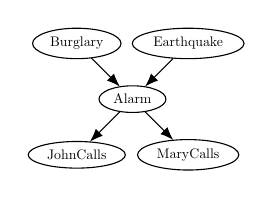
\begin{tikzpicture}[node distance=2cm,scale=0.5,every node/.style={scale=0.5}]
          \node[draw,ellipse] (alarm) {Alarm};
          \node[draw,ellipse,above left of=alarm] (burglary) {Burglary};
          \node[draw,ellipse,above right of=alarm] (earthquake) {Earthquake};
          \node[draw,ellipse,below left of=alarm] (johnCalls) {JohnCalls};
          \node[draw,ellipse,below right of=alarm] (maryCalls) {MaryCalls};
          \draw[-Latex] (burglary) -- (alarm);
          \draw[-Latex] (earthquake) -- (alarm);
          \draw[-Latex] (alarm) -- (johnCalls);
          \draw[-Latex] (alarm) -- (maryCalls);
        \end{tikzpicture}
      \end{block}
      \vspace{1cm}
      \begin{block}{Markov Random Field}
        \centering
        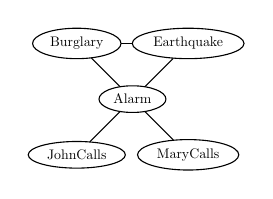
\begin{tikzpicture}[node distance=2cm,scale=0.5,every node/.style={scale=0.5}]
          \node[draw,ellipse] (alarm) {Alarm};
          \node[draw,ellipse,above left of=alarm] (burglary) {Burglary};
          \node[draw,ellipse,above right of=alarm] (earthquake) {Earthquake};
          \node[draw,ellipse,below left of=alarm] (johnCalls) {JohnCalls};
          \node[draw,ellipse,below right of=alarm] (maryCalls) {MaryCalls};
          \draw (burglary) -- (earthquake);
          \draw (burglary) -- (alarm);
          \draw (earthquake) -- (alarm);
          \draw (alarm) -- (johnCalls);
          \draw (alarm) -- (maryCalls);
        \end{tikzpicture}
      \end{block}
    \end{column}
  \end{columns}
  \onslide<2>{
    \begin{tikzpicture}[remember picture,overlay]
      \node[draw,star,fill=red!10] (wmc) at (current page.center) {WMC};
      \coordinate[xshift=-0.25\linewidth,yshift=-0.25\textheight] (p1) at (current page.center);
      \coordinate[xshift=0.25\linewidth,yshift=-0.25\textheight] (p2) at (current page.center);
      \coordinate[xshift=-0.25\linewidth,yshift=0.25\textheight] (p3) at (current page.center);
      \coordinate[xshift=0.25\linewidth,yshift=0.25\textheight] (p4) at (current page.center);
      \draw[-latex,line width=2pt,color=red!50] (p1) -- (wmc);
      \draw[-latex,line width=2pt,color=red!50] (p2) -- (wmc);
      \draw[-latex,line width=2pt,color=red!50] (p3) -- (wmc);
      \draw[-latex,line width=2pt,color=red!50] (p4) -- (wmc);
    \end{tikzpicture}
  }
\end{frame}

\begin{frame}[fragile]{Weighted Model Counting (WMC)}
  \begin{columns}
    \begin{column}{0.5\textwidth}
      \begin{itemize}
      \item Generalises propositional model counting ($\#\SAT{}$)
      \item Applications:
        \begin{itemize}
        \item graphical models
        \item probabilistic programming
        \item neural-symbolic artificial intelligence
        \end{itemize}
      \item Main types of algorithms:
        \begin{itemize}
        \item using knowledge compilation
        \item using a \SAT{} solver
        \item manipulating pseudo-Boolean functions
        \end{itemize}
      \end{itemize}
    \end{column}
    \begin{column}{0.5\textwidth}
      \begin{example}
      $w(x) = 0.3$, $w(\neg x) = 0.7$, $w(y) = 0.2$, $w(\neg y) = 0.8$
      \vspace{1cm}

      $\mathsf{WMC}(\alert{x \lor y}) = w(x)w(y) + w(x)w(\neg y) + w(\neg x)w(y)
      = 0.44$
      \end{example}
    \end{column}
  \end{columns}
\end{frame}

\begin{frame}
  \frametitle{Outline}
  \tableofcontents
\end{frame}

\section{The UAI Paper: Weighted Model Counting with Conditional Weights for Bayesian Networks}

\begin{frame}{An Alternative Way to Think About WMC}
  \begin{itemize}
  \item Let \structure{$V$} be the set of variables.
  \item Then \structure{$2^{2^V}$} is the Boolean algebra of propositional
    formulas.
  \end{itemize}
  \begin{definition}
    A \alert{measure} is a function \structure{$\mu\colon 2^{2^V} \to
      \mathbb{R}_{\ge 0}$} such that:
    \begin{itemize}
    \item \structure{$\mu(\bot) = 0$};
    \item \structure{$\mu(x \lor y) = \mu(x) + \mu(y)$} whenever \structure{$x
        \land y = \bot$}.
    \end{itemize}
  \end{definition}
  \begin{block}{Observation}
    WMC corresponds to the process of calculating the value of
    \structure{$\mu(x)$} for some \structure{$x \in 2^{2^V}$}.
  \end{block}
\end{frame}

\begin{frame}{The Limitations and Capabilities of WMC}
  \begin{alertblock}{Observation}
    Classical WMC is only able to evaluate \structure{factorable} measures
    (c.f., a collection of mutually independent random variables).
  \end{alertblock}
  \begin{theorem}[Informal Version]
    It is always possible to add more variables to turn a non-factorable measure
    into a factorable measure.
  \end{theorem}
  However, that is not necessarily a good idea!
\end{frame}

\begin{frame}{Experimental Results}
  \centering
  \input{../../../published/wmc-without-parameters/doc/long_talk/cumulative2}
\end{frame}

\section{The SAT Paper: Weighted Model Counting Without Parameter Variables}

\begin{frame}{Formalising the Intuition from Before}
  For any propositional formula \structure{$\phi$} over a set of variables
  \structure{$X$} and \structure{$p, q \in \mathbb{R}$}, let
  \structure{$[\phi]^p_q\colon 2^X \to \mathbb{R}$} be the pseudo-Boolean
  function defined as
  \[
    [\phi]^p_q(Y) \coloneqq
    \begin{cases}
      p & \text{if } Y \models \phi \\
      q & \text{otherwise}
    \end{cases}
  \]
  for any \structure{$Y \subseteq X$}.

  \begin{definition}[Pseudo-Boolean Projection (PBP)]
    A \alert{PBP instance} is a tuple \structure{$(F, X, \omega)$}, where
    \structure{$X$} is the set of variables, \structure{$F$} is a set of
    two-valued pseudo-Boolean functions \structure{$2^X \to \mathbb{R}$}, and
    \structure{$\omega \in \mathbb{R}$} is the scaling factor.
  \end{definition}
\end{frame}

\begin{frame}{From WMC to PBP}
  The WMC instance has \structure{$x$} as the only \alert{indicator} variable
  and \structure{$p$}, \structure{$q$} as \alert{parameter} variables with
  weights \structure{$w(p) = 0.2$}, \structure{$w(q) = 0.8$}, and
  \structure{$w(\neg p) = w(\neg q) = 1$}.
  \begin{center}
    \begin{tabular}{llll}
      \toprule
      WMC Clause & \onslide<2->{In CNF} & \onslide<3->{Pseudo-Boolean Function} & \\
      \midrule
      $\neg x \Rightarrow p$ & \onslide<2->{$x \lor p$} & \onslide<3->{$[\neg x]_1^{0.2}$} & \\
      $p \Rightarrow \neg x$ & \onslide<2->{$\neg x \lor \neg p$} & & \onslide<4->{$[x]^{0.8}_{0.2}$} \\
      $x \Rightarrow q$ & \onslide<2->{$\neg x \lor q$} & \onslide<3->{$[x]_1^{0.8}$} & \\
      $q \Rightarrow x$ & \onslide<2->{$x \lor \neg q$} & & \\
      $\neg x$ & \onslide<2->{$\neg x$} & \onslide<3->{$[\neg x]_0^1$} & \onslide<4->{$[\neg x]_0^1$} \\
      \bottomrule
    \end{tabular}
  \end{center}
\end{frame}

\begin{frame}{Experimental Results}
  % Created by tikzDevice version 0.12.3.1 on 2021-02-09 19:25:55
% !TEX encoding = UTF-8 Unicode
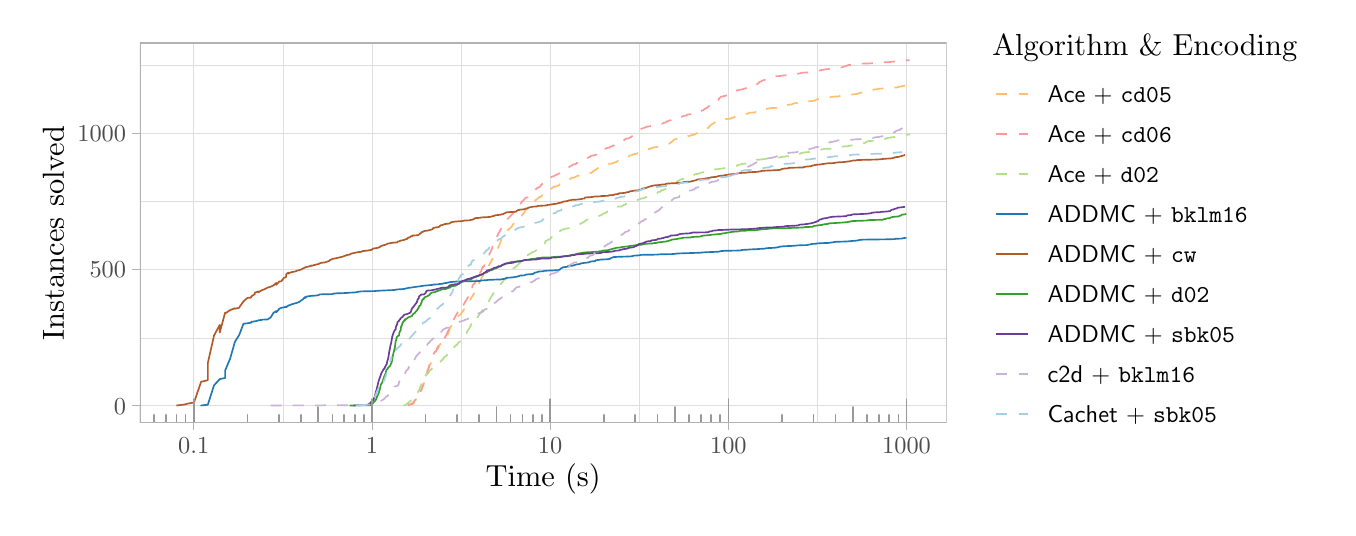
\begin{tikzpicture}[x=1pt,y=1pt]
\definecolor{fillColor}{RGB}{255,255,255}
\path[use as bounding box,fill=fillColor,fill opacity=0.00] (0,0) rectangle (469.75,173.45);
\begin{scope}
\path[clip] (  0.00,  0.00) rectangle (469.75,173.45);
\definecolor{drawColor}{RGB}{255,255,255}
\definecolor{fillColor}{RGB}{255,255,255}

\path[draw=drawColor,line width= 0.6pt,line join=round,line cap=round,fill=fillColor] (  0.00,  0.00) rectangle (469.76,173.45);
\end{scope}
\begin{scope}
\path[clip] ( 40.51, 30.69) rectangle (332.10,167.95);
\definecolor{fillColor}{RGB}{255,255,255}

\path[fill=fillColor] ( 40.51, 30.69) rectangle (332.10,167.95);
\definecolor{drawColor}{gray}{0.87}

\path[draw=drawColor,line width= 0.1pt,line join=round] ( 40.51, 61.43) --
	(332.10, 61.43);

\path[draw=drawColor,line width= 0.1pt,line join=round] ( 40.51,110.63) --
	(332.10,110.63);

\path[draw=drawColor,line width= 0.1pt,line join=round] ( 40.51,159.84) --
	(332.10,159.84);

\path[draw=drawColor,line width= 0.1pt,line join=round] ( 92.20, 30.69) --
	( 92.20,167.95);

\path[draw=drawColor,line width= 0.1pt,line join=round] (156.60, 30.69) --
	(156.60,167.95);

\path[draw=drawColor,line width= 0.1pt,line join=round] (220.99, 30.69) --
	(220.99,167.95);

\path[draw=drawColor,line width= 0.1pt,line join=round] (285.39, 30.69) --
	(285.39,167.95);

\path[draw=drawColor,line width= 0.3pt,line join=round] ( 40.51, 36.83) --
	(332.10, 36.83);

\path[draw=drawColor,line width= 0.3pt,line join=round] ( 40.51, 86.03) --
	(332.10, 86.03);

\path[draw=drawColor,line width= 0.3pt,line join=round] ( 40.51,135.24) --
	(332.10,135.24);

\path[draw=drawColor,line width= 0.3pt,line join=round] ( 60.00, 30.69) --
	( 60.00,167.95);

\path[draw=drawColor,line width= 0.3pt,line join=round] (124.40, 30.69) --
	(124.40,167.95);

\path[draw=drawColor,line width= 0.3pt,line join=round] (188.80, 30.69) --
	(188.80,167.95);

\path[draw=drawColor,line width= 0.3pt,line join=round] (253.19, 30.69) --
	(253.19,167.95);

\path[draw=drawColor,line width= 0.3pt,line join=round] (317.59, 30.69) --
	(317.59,167.95);
\definecolor{drawColor}{RGB}{253,191,111}

\path[draw=drawColor,line width= 0.6pt,dash pattern=on 4pt off 4pt ,line join=round] (137.89, 37.02) --
	(138.06, 37.12) --
	(138.23, 37.22) --
	(138.57, 37.52) --
	(138.57, 37.32) --
	(138.74, 37.61) --
	(138.91, 37.81) --
	(138.91, 37.71) --
	(139.24, 38.11) --
	(139.24, 38.20) --
	(139.57, 38.30) --
	(139.73, 38.60) --
	(139.89, 38.79) --
	(140.05, 38.89) --
	(140.84, 39.29) --
	(140.84, 39.09) --
	(140.84, 39.39) --
	(140.99, 39.48) --
	(141.15, 39.68) --
	(141.30, 39.88) --
	(141.30, 39.98) --
	(141.60, 40.27) --
	(141.60, 40.76) --
	(141.76, 40.96) --
	(141.76, 41.06) --
	(141.91, 41.55) --
	(141.91, 41.65) --
	(142.05, 41.94) --
	(142.20, 42.24) --
	(142.35, 42.53) --
	(142.50, 43.03) --
	(142.50, 42.93) --
	(142.64, 43.81) --
	(142.79, 44.11) --
	(142.79, 44.01) --
	(142.93, 44.40) --
	(143.08, 44.70) --
	(143.08, 44.60) --
	(143.22, 45.09) --
	(143.36, 45.78) --
	(143.50, 46.47) --
	(143.64, 46.86) --
	(143.78, 47.06) --
	(143.92, 47.85) --
	(144.06, 48.24) --
	(144.20, 48.34) --
	(144.20, 48.64) --
	(144.34, 49.03) --
	(144.48, 49.62) --
	(144.61, 49.92) --
	(144.75, 50.11) --
	(144.75, 50.01) --
	(144.88, 50.51) --
	(145.02, 50.80) --
	(145.15, 51.00) --
	(145.28, 51.49) --
	(145.41, 51.78) --
	(145.55, 51.88) --
	(145.68, 52.08) --
	(145.68, 52.57) --
	(145.81, 53.16) --
	(145.94, 53.46) --
	(146.07, 53.85) --
	(146.19, 54.05) --
	(146.32, 54.34) --
	(146.58, 54.64) --
	(146.70, 54.84) --
	(146.70, 54.93) --
	(146.83, 55.23) --
	(146.95, 55.62) --
	(147.08, 55.92) --
	(147.20, 56.02) --
	(147.33, 56.21) --
	(147.45, 56.31) --
	(147.57, 56.51) --
	(147.69, 56.90) --
	(147.81, 57.10) --
	(148.18, 57.39) --
	(148.29, 57.49) --
	(148.41, 57.59) --
	(148.41, 57.79) --
	(148.53, 58.08) --
	(148.65, 58.58) --
	(148.77, 58.67) --
	(148.88, 58.77) --
	(149.00, 58.97) --
	(149.12, 59.07) --
	(149.35, 59.17) --
	(149.57, 59.26) --
	(149.69, 59.56) --
	(149.80, 59.85) --
	(149.91, 60.05) --
	(150.14, 60.15) --
	(150.25, 60.25) --
	(150.36, 60.35) --
	(150.47, 60.54) --
	(150.69, 60.64) --
	(150.80, 60.74) --
	(151.01, 60.94) --
	(151.12, 61.13) --
	(151.23, 61.23) --
	(151.34, 61.63) --
	(151.44, 61.92) --
	(151.55, 62.12) --
	(151.65, 62.22) --
	(151.65, 62.41) --
	(151.76, 62.51) --
	(151.87, 62.81) --
	(152.07, 63.20) --
	(152.18, 63.69) --
	(152.28, 64.18) --
	(152.38, 64.28) --
	(152.49, 64.58) --
	(152.59, 64.97) --
	(152.69, 65.07) --
	(152.79, 65.27) --
	(152.89, 65.37) --
	(153.09, 65.66) --
	(153.19, 65.86) --
	(153.29, 66.05) --
	(153.49, 66.25) --
	(153.59, 66.35) --
	(153.69, 66.45) --
	(153.79, 66.74) --
	(153.89, 66.84) --
	(153.98, 67.04) --
	(154.18, 67.24) --
	(154.27, 67.43) --
	(154.37, 67.63) --
	(154.56, 67.73) --
	(154.75, 67.83) --
	(154.84, 67.92) --
	(155.03, 68.32) --
	(155.12, 68.61) --
	(155.40, 68.71) --
	(155.49, 68.91) --
	(155.59, 69.20) --
	(155.77, 69.30) --
	(155.77, 69.40) --
	(155.95, 69.50) --
	(156.04, 69.60) --
	(156.22, 69.70) --
	(156.31, 69.79) --
	(156.40, 69.89) --
	(156.49, 69.99) --
	(156.58, 70.09) --
	(156.67, 70.29) --
	(156.75, 70.48) --
	(156.75, 70.38) --
	(156.84, 70.58) --
	(156.93, 70.68) --
	(157.10, 70.78) --
	(157.19, 70.88) --
	(157.19, 70.97) --
	(157.28, 71.07) --
	(157.36, 71.17) --
	(157.45, 71.27) --
	(157.53, 71.37) --
	(157.62, 71.47) --
	(157.79, 71.86) --
	(157.87, 71.96) --
	(157.96, 72.06) --
	(158.04, 72.45) --
	(158.13, 72.55) --
	(158.21, 72.65) --
	(158.38, 72.75) --
	(158.54, 72.84) --
	(158.54, 72.94) --
	(158.62, 73.04) --
	(158.62, 73.24) --
	(158.71, 73.34) --
	(158.79, 73.44) --
	(158.87, 73.63) --
	(158.87, 73.73) --
	(159.11, 73.83) --
	(159.19, 73.93) --
	(159.27, 74.03) --
	(159.44, 74.42) --
	(159.52, 74.52) --
	(159.52, 74.62) --
	(159.67, 74.71) --
	(159.75, 74.81) --
	(159.91, 75.01) --
	(159.91, 75.11) --
	(160.07, 75.21) --
	(160.15, 75.40) --
	(160.22, 75.70) --
	(160.22, 75.50) --
	(160.30, 75.99) --
	(160.30, 75.80) --
	(160.46, 76.09) --
	(160.61, 76.29) --
	(160.76, 76.58) --
	(160.91, 76.68) --
	(160.99, 76.78) --
	(160.99, 77.17) --
	(161.22, 77.27) --
	(161.36, 77.47) --
	(161.44, 77.67) --
	(161.51, 77.86) --
	(161.51, 77.96) --
	(161.74, 78.06) --
	(161.88, 78.16) --
	(161.88, 78.26) --
	(162.03, 78.55) --
	(162.10, 78.75) --
	(162.17, 78.95) --
	(162.25, 79.44) --
	(162.32, 79.63) --
	(162.39, 79.83) --
	(162.39, 79.93) --
	(162.46, 80.03) --
	(162.53, 80.13) --
	(162.60, 80.23) --
	(162.68, 80.52) --
	(162.68, 80.42) --
	(162.75, 80.62) --
	(162.82, 80.82) --
	(162.89, 80.91) --
	(162.96, 81.01) --
	(163.03, 81.11) --
	(163.17, 81.21) --
	(163.24, 81.41) --
	(163.31, 81.50) --
	(163.38, 81.60) --
	(163.38, 81.80) --
	(163.45, 82.00) --
	(163.59, 82.19) --
	(163.65, 82.29) --
	(163.72, 82.39) --
	(163.79, 82.59) --
	(163.93, 82.69) --
	(164.00, 82.88) --
	(164.06, 83.08) --
	(164.20, 83.28) --
	(164.33, 83.47) --
	(164.40, 83.57) --
	(164.53, 83.77) --
	(164.60, 83.87) --
	(164.67, 83.96) --
	(164.73, 84.26) --
	(164.87, 84.36) --
	(164.93, 84.65) --
	(165.00, 84.75) --
	(165.06, 84.85) --
	(165.19, 84.95) --
	(165.26, 85.15) --
	(165.26, 85.05) --
	(165.32, 85.24) --
	(165.45, 85.54) --
	(165.71, 85.74) --
	(165.77, 85.83) --
	(165.84, 85.93) --
	(165.96, 86.03) --
	(166.15, 86.23) --
	(166.28, 86.43) --
	(166.28, 86.52) --
	(166.40, 86.82) --
	(166.53, 87.11) --
	(166.59, 87.21) --
	(166.65, 87.41) --
	(166.65, 87.31) --
	(166.71, 87.70) --
	(166.83, 87.80) --
	(166.90, 87.90) --
	(166.96, 88.00) --
	(167.02, 88.10) --
	(167.08, 88.29) --
	(167.14, 88.39) --
	(167.20, 88.49) --
	(167.32, 88.69) --
	(167.32, 88.59) --
	(167.44, 88.79) --
	(167.50, 89.08) --
	(167.56, 89.18) --
	(167.68, 89.28) --
	(167.74, 89.38) --
	(167.80, 89.77) --
	(167.80, 89.48) --
	(167.92, 89.87) --
	(167.98, 90.16) --
	(168.03, 90.26) --
	(168.09, 90.46) --
	(168.15, 90.56) --
	(168.21, 90.66) --
	(168.27, 90.76) --
	(168.33, 90.85) --
	(168.38, 91.05) --
	(168.50, 91.44) --
	(168.56, 91.54) --
	(168.67, 91.64) --
	(168.73, 91.74) --
	(168.79, 91.84) --
	(168.90, 91.94) --
	(169.02, 92.03) --
	(169.07, 92.13) --
	(169.19, 92.23) --
	(169.24, 92.33) --
	(169.35, 92.53) --
	(169.41, 92.72) --
	(169.47, 92.82) --
	(169.52, 93.02) --
	(169.63, 93.12) --
	(169.69, 93.22) --
	(169.74, 93.31) --
	(169.80, 93.41) --
	(169.85, 93.61) --
	(169.91, 93.71) --
	(170.02, 93.90) --
	(170.07, 94.20) --
	(170.18, 94.30) --
	(170.24, 94.40) --
	(170.29, 94.49) --
	(170.35, 94.69) --
	(170.45, 94.89) --
	(170.51, 94.99) --
	(170.56, 95.09) --
	(170.61, 95.28) --
	(170.67, 95.38) --
	(170.77, 95.68) --
	(170.83, 95.87) --
	(170.88, 96.17) --
	(170.88, 95.97) --
	(170.93, 96.46) --
	(170.99, 96.56) --
	(171.04, 96.66) --
	(171.09, 96.76) --
	(171.20, 96.86) --
	(171.25, 96.96) --
	(171.35, 97.05) --
	(171.67, 97.25) --
	(171.77, 97.35) --
	(172.08, 97.45) --
	(172.13, 97.55) --
	(172.18, 97.64) --
	(172.23, 97.84) --
	(172.28, 97.94) --
	(172.38, 98.04) --
	(172.43, 98.14) --
	(172.48, 98.23) --
	(172.53, 98.33) --
	(172.58, 98.53) --
	(172.63, 98.63) --
	(172.68, 98.73) --
	(172.78, 98.82) --
	(172.83, 98.92) --
	(172.88, 99.02) --
	(172.98, 99.32) --
	(173.03, 99.61) --
	(173.07, 99.81) --
	(173.17,100.01) --
	(173.22,100.10) --
	(173.32,100.20) --
	(173.56,100.30) --
	(173.66,100.40) --
	(173.75,100.60) --
	(173.90,100.69) --
	(174.23,100.89) --
	(174.23,100.79) --
	(174.32,100.99) --
	(174.42,101.09) --
	(174.46,101.19) --
	(174.65,101.29) --
	(174.74,101.38) --
	(174.83,101.48) --
	(174.88,101.58) --
	(174.93,101.68) --
	(175.06,101.88) --
	(175.15,101.97) --
	(175.20,102.07) --
	(175.20,102.17) --
	(175.25,102.27) --
	(175.38,102.37) --
	(175.43,102.47) --
	(175.61,102.56) --
	(175.74,102.66) --
	(176.01,102.76) --
	(176.09,102.86) --
	(176.18,103.06) --
	(176.31,103.15) --
	(176.40,103.25) --
	(176.53,103.45) --
	(176.57,103.55) --
	(176.66,103.65) --
	(176.79,103.75) --
	(176.83,103.84) --
	(176.88,104.04) --
	(177.00,104.14) --
	(177.43,104.24) --
	(177.51,104.34) --
	(177.55,104.43) --
	(177.68,104.53) --
	(177.72,104.63) --
	(177.72,104.73) --
	(177.80,104.83) --
	(177.89,104.93) --
	(177.89,105.02) --
	(178.09,105.12) --
	(178.26,105.22) --
	(178.30,105.32) --
	(178.54,105.42) --
	(178.58,105.52) --
	(178.66,105.71) --
	(178.78,105.81) --
	(178.82,105.91) --
	(178.90,106.01) --
	(178.98,106.11) --
	(179.14,106.21) --
	(179.22,106.30) --
	(179.26,106.40) --
	(179.41,106.50) --
	(179.45,106.60) --
	(179.49,106.80) --
	(179.53,106.89) --
	(179.61,106.99) --
	(179.65,107.09) --
	(179.69,107.19) --
	(179.72,107.29) --
	(179.76,107.39) --
	(179.80,107.48) --
	(179.92,107.58) --
	(179.99,107.68) --
	(180.41,107.78) --
	(180.49,107.98) --
	(180.79,108.17) --
	(180.82,108.27) --
	(180.90,108.37) --
	(181.12,108.47) --
	(181.19,108.67) --
	(181.19,108.57) --
	(181.27,108.86) --
	(181.27,108.76) --
	(181.30,108.96) --
	(181.34,109.06) --
	(181.41,109.16) --
	(181.74,109.26) --
	(181.81,109.35) --
	(181.81,109.45) --
	(181.95,109.55) --
	(181.99,109.65) --
	(181.99,109.75) --
	(182.10,109.85) --
	(182.13,109.95) --
	(182.24,110.04) --
	(182.41,110.14) --
	(182.87,110.24) --
	(183.01,110.34) --
	(183.11,110.44) --
	(183.18,110.54) --
	(183.25,110.63) --
	(183.38,110.73) --
	(183.42,110.83) --
	(183.48,110.93) --
	(183.52,111.03) --
	(183.58,111.13) --
	(183.62,111.22) --
	(183.68,111.32) --
	(183.92,111.42) --
	(184.02,111.52) --
	(184.18,111.62) --
	(184.35,111.72) --
	(184.61,111.81) --
	(184.64,111.91) --
	(184.67,112.11) --
	(184.74,112.21) --
	(185.35,112.31) --
	(185.50,112.41) --
	(185.63,112.50) --
	(185.66,112.70) --
	(186.00,112.80) --
	(186.13,112.90) --
	(186.16,113.00) --
	(186.83,113.09) --
	(186.95,113.19) --
	(187.21,113.29) --
	(187.51,113.39) --
	(187.54,113.49) --
	(187.57,113.59) --
	(187.60,113.68) --
	(187.71,113.78) --
	(187.80,113.88) --
	(187.89,113.98) --
	(187.91,114.08) --
	(188.17,114.18) --
	(188.37,114.28) --
	(188.49,114.37) --
	(188.63,114.47) --
	(188.68,114.57) --
	(188.85,114.67) --
	(189.02,114.77) --
	(189.07,114.87) --
	(189.10,115.06) --
	(189.16,115.16) --
	(189.24,115.26) --
	(189.35,115.36) --
	(189.49,115.46) --
	(189.54,115.55) --
	(189.59,115.65) --
	(189.78,115.75) --
	(189.92,115.85) --
	(190.16,115.95) --
	(190.45,116.05) --
	(191.21,116.15) --
	(191.41,116.24) --
	(191.49,116.34) --
	(191.91,116.44) --
	(191.96,116.54) --
	(192.11,116.64) --
	(192.19,116.74) --
	(192.26,116.83) --
	(192.66,116.93) --
	(192.87,117.13) --
	(192.95,117.23) --
	(193.04,117.33) --
	(193.09,117.42) --
	(193.11,117.52) --
	(193.23,117.62) --
	(193.57,117.72) --
	(193.78,117.82) --
	(194.13,117.92) --
	(194.70,118.01) --
	(194.92,118.11) --
	(195.15,118.21) --
	(195.26,118.31) --
	(195.66,118.41) --
	(195.70,118.51) --
	(195.98,118.61) --
	(196.00,118.70) --
	(196.07,118.80) --
	(196.13,118.90) --
	(196.39,119.10) --
	(197.06,119.20) --
	(197.33,119.29) --
	(197.66,119.39) --
	(197.82,119.49) --
	(197.84,119.59) --
	(198.32,119.69) --
	(198.46,119.79) --
	(198.62,119.88) --
	(199.15,119.98) --
	(199.44,120.08) --
	(199.47,120.18) --
	(199.57,120.28) --
	(199.83,120.38) --
	(199.89,120.48) --
	(200.02,120.57) --
	(200.87,120.67) --
	(201.52,120.77) --
	(201.68,120.87) --
	(203.70,120.97) --
	(203.78,121.07) --
	(203.96,121.16) --
	(203.98,121.26) --
	(204.11,121.36) --
	(204.25,121.46) --
	(204.37,121.66) --
	(204.68,121.75) --
	(204.87,121.85) --
	(205.09,121.95) --
	(205.11,122.05) --
	(205.36,122.15) --
	(205.57,122.25) --
	(205.60,122.34) --
	(205.62,122.44) --
	(205.74,122.54) --
	(205.98,122.64) --
	(206.03,122.74) --
	(206.46,122.84) --
	(206.51,122.94) --
	(206.73,123.03) --
	(206.83,123.13) --
	(207.05,123.23) --
	(207.96,123.33) --
	(208.35,123.43) --
	(208.93,123.53) --
	(209.16,123.62) --
	(209.17,123.72) --
	(209.21,123.82) --
	(209.25,123.92) --
	(209.42,124.02) --
	(209.90,124.12) --
	(209.94,124.21) --
	(210.56,124.31) --
	(211.45,124.41) --
	(211.60,124.51) --
	(211.75,124.61) --
	(212.11,124.71) --
	(212.21,124.81) --
	(212.71,124.90) --
	(212.89,125.00) --
	(212.97,125.10) --
	(213.02,125.20) --
	(213.24,125.30) --
	(213.40,125.40) --
	(213.45,125.49) --
	(213.58,125.59) --
	(214.25,125.69) --
	(214.44,125.79) --
	(214.58,125.89) --
	(214.70,125.99) --
	(215.02,126.08) --
	(215.19,126.18) --
	(215.46,126.28) --
	(216.35,126.38) --
	(216.45,126.48) --
	(216.85,126.58) --
	(216.99,126.67) --
	(217.11,126.77) --
	(217.25,126.87) --
	(217.31,126.97) --
	(217.42,127.07) --
	(217.43,127.17) --
	(217.52,127.27) --
	(218.20,127.36) --
	(218.54,127.46) --
	(218.58,127.56) --
	(218.70,127.66) --
	(219.29,127.76) --
	(219.84,127.86) --
	(220.21,127.95) --
	(220.22,128.05) --
	(220.38,128.15) --
	(220.45,128.25) --
	(220.56,128.35) --
	(220.73,128.45) --
	(220.95,128.54) --
	(220.98,128.64) --
	(221.16,128.74) --
	(221.56,128.84) --
	(221.77,128.94) --
	(221.86,129.04) --
	(222.58,129.14) --
	(222.59,129.23) --
	(222.68,129.33) --
	(224.16,129.43) --
	(224.38,129.53) --
	(224.44,129.63) --
	(225.03,129.73) --
	(225.16,129.82) --
	(225.22,129.92) --
	(226.29,130.12) --
	(226.31,130.22) --
	(227.47,130.32) --
	(227.84,130.41) --
	(228.31,130.51) --
	(228.38,130.61) --
	(228.59,130.71) --
	(229.06,130.81) --
	(229.73,130.91) --
	(229.96,131.00) --
	(230.12,131.10) --
	(231.07,131.20) --
	(231.14,131.30) --
	(231.20,131.40) --
	(231.82,131.50) --
	(231.90,131.60) --
	(232.01,131.69) --
	(232.11,131.79) --
	(232.46,131.89) --
	(232.46,131.99) --
	(232.48,132.09) --
	(232.72,132.19) --
	(232.98,132.28) --
	(233.06,132.38) --
	(233.07,132.48) --
	(233.09,132.58) --
	(233.21,132.68) --
	(233.43,132.78) --
	(233.46,132.87) --
	(233.59,132.97) --
	(233.79,133.07) --
	(234.04,133.17) --
	(234.47,133.27) --
	(234.96,133.37) --
	(235.29,133.47) --
	(236.12,133.56) --
	(236.25,133.66) --
	(236.50,133.76) --
	(236.61,133.86) --
	(237.13,133.96) --
	(237.16,134.06) --
	(238.50,134.15) --
	(238.52,134.25) --
	(239.16,134.35) --
	(239.66,134.45) --
	(239.68,134.55) --
	(239.88,134.65) --
	(240.96,134.74) --
	(240.97,134.84) --
	(241.22,134.94) --
	(241.28,135.04) --
	(241.42,135.14) --
	(241.61,135.24) --
	(241.83,135.33) --
	(242.08,135.43) --
	(242.17,135.53) --
	(242.84,135.63) --
	(242.91,135.73) --
	(243.08,135.83) --
	(243.22,135.93) --
	(243.72,136.02) --
	(243.81,136.12) --
	(243.88,136.22) --
	(243.92,136.32) --
	(244.16,136.42) --
	(244.35,136.52) --
	(244.52,136.61) --
	(244.59,136.71) --
	(245.22,136.81) --
	(245.39,136.91) --
	(245.42,137.01) --
	(245.54,137.11) --
	(245.97,137.20) --
	(246.03,137.30) --
	(246.06,137.40) --
	(246.07,137.50) --
	(246.16,137.60) --
	(246.35,137.70) --
	(246.37,137.80) --
	(246.43,137.89) --
	(246.44,137.99) --
	(246.66,138.09) --
	(246.69,138.19) --
	(246.85,138.29) --
	(246.96,138.39) --
	(247.12,138.48) --
	(247.18,138.58) --
	(247.36,138.68) --
	(247.58,138.78) --
	(248.09,138.88) --
	(248.09,138.98) --
	(248.13,139.07) --
	(248.19,139.17) --
	(248.34,139.27) --
	(248.36,139.37) --
	(248.54,139.47) --
	(248.72,139.57) --
	(248.83,139.66) --
	(248.99,139.76) --
	(249.27,139.86) --
	(249.92,139.96) --
	(250.26,140.06) --
	(250.36,140.16) --
	(250.40,140.26) --
	(251.10,140.35) --
	(252.40,140.45) --
	(253.61,140.55) --
	(254.15,140.65) --
	(254.22,140.75) --
	(254.34,140.85) --
	(255.23,140.94) --
	(255.24,141.04) --
	(255.31,141.14) --
	(255.39,141.24) --
	(255.67,141.34) --
	(255.94,141.44) --
	(256.47,141.53) --
	(256.76,141.63) --
	(256.85,141.73) --
	(257.55,141.83) --
	(257.96,141.93) --
	(258.17,142.03) --
	(258.34,142.13) --
	(259.62,142.22) --
	(259.65,142.32) --
	(260.28,142.42) --
	(260.58,142.52) --
	(260.58,142.62) --
	(260.61,142.72) --
	(262.84,142.81) --
	(262.89,142.91) --
	(263.01,143.01) --
	(263.23,143.11) --
	(263.40,143.21) --
	(263.79,143.31) --
	(263.87,143.40) --
	(264.02,143.50) --
	(265.44,143.60) --
	(265.47,143.70) --
	(266.26,143.80) --
	(266.28,143.90) --
	(267.04,144.00) --
	(267.05,144.09) --
	(267.20,144.19) --
	(268.09,144.29) --
	(268.58,144.39) --
	(270.72,144.49) --
	(270.88,144.59) --
	(270.88,144.68) --
	(271.09,144.78) --
	(271.46,144.88) --
	(272.69,144.98) --
	(272.85,145.08) --
	(272.85,145.18) --
	(272.91,145.27) --
	(272.92,145.37) --
	(274.05,145.47) --
	(274.71,145.57) --
	(275.84,145.67) --
	(276.17,145.77) --
	(276.20,145.86) --
	(276.57,145.96) --
	(276.80,146.06) --
	(277.17,146.16) --
	(278.09,146.26) --
	(278.24,146.36) --
	(279.30,146.46) --
	(279.70,146.55) --
	(281.29,146.65) --
	(282.02,146.75) --
	(282.02,146.85) --
	(283.33,146.95) --
	(284.38,147.05) --
	(284.56,147.14) --
	(284.58,147.24) --
	(284.79,147.34) --
	(284.93,147.44) --
	(285.10,147.54) --
	(285.58,147.64) --
	(285.73,147.73) --
	(286.44,147.83) --
	(287.73,147.93) --
	(288.47,148.03) --
	(288.94,148.13) --
	(289.34,148.23) --
	(290.02,148.33) --
	(290.18,148.42) --
	(291.16,148.52) --
	(293.13,148.62) --
	(293.18,148.72) --
	(294.88,148.82) --
	(294.97,148.92) --
	(295.36,149.01) --
	(296.84,149.11) --
	(297.65,149.21) --
	(297.89,149.31) --
	(298.85,149.41) --
	(299.73,149.51) --
	(299.90,149.60) --
	(300.21,149.70) --
	(300.55,149.80) --
	(300.75,149.90) --
	(301.09,150.00) --
	(302.02,150.10) --
	(302.69,150.19) --
	(303.66,150.29) --
	(303.94,150.39) --
	(304.07,150.49) --
	(304.23,150.59) --
	(304.30,150.69) --
	(305.19,150.79) --
	(305.42,150.88) --
	(305.52,150.98) --
	(305.71,151.08) --
	(306.58,151.18) --
	(307.17,151.28) --
	(307.34,151.38) --
	(309.13,151.47) --
	(309.89,151.57) --
	(310.81,151.67) --
	(312.46,151.77) --
	(314.33,151.87) --
	(314.39,151.97) --
	(314.58,152.06) --
	(315.47,152.16) --
	(315.67,152.26) --
	(316.25,152.36) --
	(316.87,152.46) --
	(317.40,152.56);
\definecolor{drawColor}{RGB}{251,154,153}

\path[draw=drawColor,line width= 0.6pt,dash pattern=on 4pt off 4pt ,line join=round] (137.37, 36.93) --
	(137.54, 37.02) --
	(137.72, 37.22) --
	(137.89, 37.32) --
	(138.57, 37.42) --
	(139.24, 37.52) --
	(139.40, 37.61) --
	(139.57, 38.11) --
	(139.73, 38.40) --
	(139.89, 38.79) --
	(140.05, 38.89) --
	(140.21, 39.09) --
	(140.21, 38.99) --
	(140.37, 39.29) --
	(140.53, 39.48) --
	(140.53, 39.39) --
	(140.68, 39.88) --
	(140.84, 40.07) --
	(140.99, 40.27) --
	(141.15, 40.76) --
	(141.30, 40.96) --
	(141.45, 41.26) --
	(141.45, 41.06) --
	(141.60, 41.35) --
	(141.60, 41.55) --
	(141.76, 41.65) --
	(141.76, 41.75) --
	(141.91, 42.14) --
	(141.91, 42.04) --
	(142.05, 42.44) --
	(142.05, 42.53) --
	(142.20, 42.73) --
	(142.20, 42.83) --
	(142.35, 43.12) --
	(142.50, 43.32) --
	(142.50, 43.22) --
	(142.64, 43.52) --
	(142.79, 44.01) --
	(142.79, 43.81) --
	(142.93, 44.40) --
	(143.08, 44.99) --
	(143.08, 44.60) --
	(143.22, 45.29) --
	(143.36, 45.78) --
	(143.50, 46.18) --
	(143.64, 46.67) --
	(143.78, 46.96) --
	(143.92, 47.36) --
	(143.92, 47.45) --
	(144.06, 48.05) --
	(144.20, 48.34) --
	(144.20, 48.44) --
	(144.34, 48.73) --
	(144.48, 49.32) --
	(144.61, 49.72) --
	(144.75, 50.01) --
	(144.75, 50.11) --
	(144.88, 50.60) --
	(145.02, 51.00) --
	(145.15, 51.59) --
	(145.28, 51.88) --
	(145.41, 52.18) --
	(145.55, 52.57) --
	(145.68, 53.06) --
	(145.81, 53.26) --
	(145.94, 53.65) --
	(146.07, 54.15) --
	(146.19, 54.25) --
	(146.19, 54.34) --
	(146.32, 54.64) --
	(146.45, 54.93) --
	(146.58, 55.43) --
	(146.70, 55.62) --
	(146.83, 55.72) --
	(146.95, 56.11) --
	(147.08, 56.21) --
	(147.20, 56.31) --
	(147.33, 56.41) --
	(147.45, 56.51) --
	(147.69, 56.90) --
	(147.81, 57.39) --
	(147.94, 57.49) --
	(147.94, 57.69) --
	(148.06, 57.79) --
	(148.18, 58.18) --
	(148.29, 58.28) --
	(148.41, 58.38) --
	(148.53, 58.58) --
	(148.65, 58.67) --
	(148.77, 58.77) --
	(149.12, 59.17) --
	(149.23, 59.26) --
	(149.35, 59.36) --
	(149.35, 59.46) --
	(149.46, 59.56) --
	(149.57, 59.85) --
	(149.69, 59.95) --
	(149.80, 60.05) --
	(149.91, 60.25) --
	(150.03, 60.44) --
	(150.14, 60.54) --
	(150.25, 60.84) --
	(150.25, 60.64) --
	(150.36, 60.94) --
	(150.58, 61.23) --
	(150.69, 61.63) --
	(150.69, 61.33) --
	(150.91, 61.72) --
	(151.01, 61.92) --
	(151.12, 62.12) --
	(151.23, 62.31) --
	(151.23, 62.41) --
	(151.34, 62.61) --
	(151.44, 62.91) --
	(151.55, 63.00) --
	(151.65, 63.30) --
	(151.76, 63.59) --
	(151.87, 63.79) --
	(151.97, 63.89) --
	(152.07, 64.18) --
	(152.18, 64.38) --
	(152.28, 64.48) --
	(152.38, 64.87) --
	(152.49, 64.97) --
	(152.59, 65.17) --
	(152.69, 65.46) --
	(152.89, 65.76) --
	(153.09, 66.15) --
	(153.19, 66.25) --
	(153.29, 66.55) --
	(153.39, 66.74) --
	(153.49, 66.94) --
	(153.59, 67.24) --
	(153.79, 67.53) --
	(153.79, 67.43) --
	(153.89, 67.83) --
	(153.98, 68.12) --
	(154.08, 68.22) --
	(154.18, 68.51) --
	(154.18, 68.32) --
	(154.27, 68.61) --
	(154.37, 68.81) --
	(154.46, 69.01) --
	(154.46, 68.91) --
	(154.56, 69.20) --
	(154.56, 69.11) --
	(154.65, 69.40) --
	(154.75, 69.50) --
	(154.84, 69.70) --
	(154.94, 69.89) --
	(155.03, 69.99) --
	(155.12, 70.09) --
	(155.22, 70.19) --
	(155.31, 70.48) --
	(155.59, 70.68) --
	(155.68, 70.88) --
	(155.86, 70.97) --
	(156.04, 71.07) --
	(156.04, 71.17) --
	(156.22, 71.27) --
	(156.31, 71.37) --
	(156.49, 71.47) --
	(156.67, 71.76) --
	(156.75, 71.96) --
	(156.75, 71.86) --
	(156.84, 72.06) --
	(156.93, 72.16) --
	(157.02, 72.55) --
	(157.10, 72.75) --
	(157.10, 72.65) --
	(157.19, 72.94) --
	(157.19, 73.04) --
	(157.28, 73.14) --
	(157.53, 73.44) --
	(157.53, 73.24) --
	(157.62, 73.53) --
	(157.62, 73.63) --
	(157.79, 73.73) --
	(157.87, 74.03) --
	(157.87, 73.93) --
	(157.96, 74.12) --
	(157.96, 74.32) --
	(158.04, 74.42) --
	(158.21, 74.52) --
	(158.29, 74.62) --
	(158.29, 74.71) --
	(158.46, 74.91) --
	(158.54, 75.01) --
	(158.54, 75.11) --
	(158.62, 75.30) --
	(158.79, 75.60) --
	(158.87, 75.70) --
	(158.95, 75.80) --
	(159.11, 75.99) --
	(159.27, 76.19) --
	(159.36, 76.29) --
	(159.44, 76.49) --
	(159.67, 76.58) --
	(159.75, 76.78) --
	(159.83, 77.17) --
	(159.91, 77.37) --
	(159.91, 77.57) --
	(159.99, 77.67) --
	(160.07, 78.06) --
	(160.15, 78.36) --
	(160.22, 78.45) --
	(160.30, 78.55) --
	(160.38, 78.85) --
	(160.46, 79.14) --
	(160.53, 79.44) --
	(160.61, 79.73) --
	(160.61, 79.54) --
	(160.76, 80.13) --
	(160.84, 80.42) --
	(160.84, 80.32) --
	(160.91, 80.52) --
	(160.99, 80.62) --
	(161.22, 80.72) --
	(161.29, 80.82) --
	(161.36, 81.01) --
	(161.44, 81.11) --
	(161.59, 81.21) --
	(161.74, 81.31) --
	(161.81, 81.60) --
	(161.88, 81.80) --
	(161.88, 81.70) --
	(161.96, 81.90) --
	(162.10, 82.10) --
	(162.17, 82.29) --
	(162.17, 82.19) --
	(162.25, 82.49) --
	(162.39, 82.59) --
	(162.46, 82.69) --
	(162.46, 82.78) --
	(162.53, 82.88) --
	(162.60, 83.08) --
	(162.68, 83.28) --
	(162.89, 83.37) --
	(162.96, 83.47) --
	(163.03, 83.77) --
	(163.03, 83.57) --
	(163.10, 84.26) --
	(163.10, 83.87) --
	(163.17, 84.56) --
	(163.38, 84.65) --
	(163.38, 84.75) --
	(163.45, 84.85) --
	(163.52, 85.05) --
	(163.59, 85.24) --
	(163.59, 85.15) --
	(163.79, 85.34) --
	(163.86, 85.44) --
	(164.00, 85.74) --
	(164.06, 86.23) --
	(164.13, 86.33) --
	(164.13, 86.43) --
	(164.20, 86.52) --
	(164.27, 86.62) --
	(164.40, 86.72) --
	(164.47, 86.92) --
	(164.47, 87.02) --
	(164.53, 87.11) --
	(164.73, 87.21) --
	(164.93, 87.31) --
	(165.00, 87.41) --
	(165.06, 87.70) --
	(165.13, 87.90) --
	(165.19, 88.29) --
	(165.26, 88.39) --
	(165.39, 88.49) --
	(165.45, 88.89) --
	(165.52, 88.98) --
	(165.58, 89.08) --
	(165.71, 89.38) --
	(165.84, 89.48) --
	(165.96, 89.57) --
	(166.03, 89.67) --
	(166.09, 89.77) --
	(166.09, 89.87) --
	(166.15, 90.07) --
	(166.15, 89.97) --
	(166.21, 90.26) --
	(166.28, 90.36) --
	(166.34, 90.46) --
	(166.46, 90.76) --
	(166.59, 91.05) --
	(166.71, 91.15) --
	(166.77, 91.35) --
	(166.90, 91.84) --
	(166.96, 91.94) --
	(167.02, 92.03) --
	(167.14, 92.13) --
	(167.20, 92.23) --
	(167.26, 92.43) --
	(167.32, 92.63) --
	(167.38, 92.82) --
	(167.38, 92.72) --
	(167.50, 93.02) --
	(167.56, 93.22) --
	(167.62, 93.31) --
	(167.74, 93.51) --
	(167.80, 93.71) --
	(167.86, 93.90) --
	(167.86, 93.81) --
	(167.92, 94.10) --
	(167.98, 94.40) --
	(168.03, 94.49) --
	(168.09, 94.59) --
	(168.15, 94.79) --
	(168.15, 94.89) --
	(168.21, 95.18) --
	(168.27, 95.38) --
	(168.33, 95.58) --
	(168.38, 95.68) --
	(168.44, 95.77) --
	(168.50, 95.87) --
	(168.62, 95.97) --
	(168.62, 96.07) --
	(168.67, 96.17) --
	(168.79, 96.27) --
	(168.85, 96.36) --
	(168.96, 96.46) --
	(169.02, 96.66) --
	(169.07, 96.76) --
	(169.13, 96.86) --
	(169.19, 97.25) --
	(169.24, 97.35) --
	(169.30, 97.55) --
	(169.30, 97.45) --
	(169.35, 97.64) --
	(169.47, 97.74) --
	(169.52, 97.94) --
	(169.63, 98.04) --
	(169.69, 98.23) --
	(169.74, 98.33) --
	(169.80, 98.43) --
	(169.91, 98.53) --
	(169.96, 98.73) --
	(170.02, 98.92) --
	(170.07, 99.22) --
	(170.24, 99.32) --
	(170.35, 99.51) --
	(170.40, 99.61) --
	(170.51, 99.71) --
	(170.56, 99.81) --
	(170.67,100.20) --
	(170.67,100.01) --
	(170.83,100.30) --
	(170.88,100.40) --
	(170.93,100.60) --
	(171.04,100.69) --
	(171.09,100.79) --
	(171.15,100.89) --
	(171.20,100.99) --
	(171.25,101.09) --
	(171.30,101.38) --
	(171.41,101.58) --
	(171.46,101.68) --
	(171.56,101.78) --
	(171.61,101.88) --
	(171.77,101.97) --
	(171.87,102.07) --
	(171.92,102.27) --
	(172.02,102.37) --
	(172.08,102.47) --
	(172.13,102.56) --
	(172.18,102.86) --
	(172.38,102.96) --
	(172.48,103.06) --
	(172.53,103.15) --
	(172.63,103.25) --
	(172.73,103.35) --
	(172.78,103.45) --
	(172.83,103.55) --
	(172.98,103.65) --
	(173.12,103.75) --
	(173.22,103.84) --
	(173.27,104.04) --
	(173.32,104.14) --
	(173.37,104.34) --
	(173.61,104.43) --
	(173.75,104.63) --
	(173.80,104.73) --
	(173.90,104.83) --
	(174.04,104.93) --
	(174.09,105.02) --
	(174.23,105.12) --
	(174.28,105.22) --
	(174.37,105.32) --
	(174.51,105.52) --
	(174.65,105.62) --
	(174.69,105.71) --
	(174.79,105.81) --
	(174.83,105.91) --
	(175.20,106.01) --
	(175.25,106.11) --
	(175.29,106.21) --
	(175.34,106.30) --
	(175.38,106.40) --
	(175.43,106.50) --
	(175.52,106.60) --
	(175.61,106.70) --
	(175.70,106.80) --
	(175.83,106.89) --
	(175.92,106.99) --
	(175.92,107.09) --
	(175.96,107.19) --
	(176.18,107.39) --
	(176.23,107.48) --
	(176.27,107.68) --
	(176.27,107.58) --
	(176.36,107.78) --
	(176.40,107.88) --
	(176.44,108.08) --
	(176.44,107.98) --
	(176.49,108.17) --
	(176.57,108.27) --
	(176.75,108.37) --
	(176.83,108.47) --
	(176.88,108.57) --
	(176.92,108.67) --
	(177.05,108.76) --
	(177.22,109.06) --
	(177.34,109.16) --
	(177.43,109.35) --
	(177.60,109.45) --
	(177.76,109.55) --
	(177.89,109.65) --
	(177.89,109.75) --
	(178.01,109.85) --
	(178.05,109.95) --
	(178.26,110.04) --
	(178.30,110.14) --
	(178.34,110.24) --
	(178.50,110.34) --
	(178.54,110.44) --
	(178.58,110.54) --
	(178.66,110.63) --
	(178.78,110.73) --
	(178.86,110.83) --
	(179.06,110.93) --
	(179.14,111.03) --
	(179.22,111.13) --
	(179.30,111.22) --
	(179.33,111.32) --
	(179.45,111.42) --
	(179.65,111.62) --
	(179.65,111.72) --
	(179.72,111.81) --
	(179.84,111.91) --
	(180.37,112.01) --
	(180.41,112.11) --
	(180.64,112.21) --
	(180.71,112.31) --
	(180.75,112.41) --
	(180.82,112.50) --
	(181.08,112.70) --
	(181.19,112.80) --
	(181.23,112.90) --
	(181.27,113.00) --
	(181.45,113.09) --
	(181.59,113.19) --
	(181.85,113.39) --
	(181.88,113.49) --
	(181.99,113.59) --
	(182.06,113.68) --
	(182.10,113.78) --
	(182.10,113.88) --
	(182.13,113.98) --
	(182.17,114.08) --
	(182.62,114.18) --
	(182.66,114.28) --
	(182.94,114.37) --
	(183.14,114.47) --
	(183.21,114.67) --
	(183.35,114.77) --
	(183.45,114.87) --
	(183.52,114.96) --
	(183.55,115.06) --
	(183.82,115.16) --
	(183.85,115.26) --
	(184.02,115.36) --
	(184.05,115.46) --
	(184.08,115.55) --
	(184.45,115.65) --
	(184.74,115.75) --
	(185.00,115.95) --
	(185.25,116.05) --
	(185.28,116.24) --
	(185.35,116.34) --
	(185.38,116.54) --
	(185.38,116.44) --
	(185.54,116.64) --
	(185.66,116.74) --
	(185.82,116.93) --
	(186.10,117.03) --
	(186.25,117.13) --
	(186.31,117.23) --
	(186.43,117.33) --
	(186.64,117.42) --
	(186.71,117.52) --
	(187.24,117.62) --
	(187.45,117.72) --
	(187.54,117.92) --
	(187.54,117.82) --
	(187.62,118.01) --
	(187.71,118.11) --
	(187.89,118.31) --
	(187.91,118.41) --
	(188.06,118.51) --
	(188.09,118.61) --
	(188.17,118.80) --
	(188.20,119.00) --
	(188.40,119.10) --
	(188.49,119.20) --
	(188.74,119.29) --
	(189.21,119.39) --
	(189.27,119.49) --
	(189.29,119.59) --
	(189.89,119.69) --
	(190.08,119.79) --
	(190.21,119.88) --
	(190.50,119.98) --
	(190.61,120.08) --
	(190.90,120.18) --
	(191.05,120.28) --
	(191.31,120.38) --
	(191.36,120.48) --
	(191.71,120.57) --
	(191.76,120.67) --
	(191.84,120.77) --
	(192.73,120.87) --
	(192.90,120.97) --
	(192.97,121.07) --
	(193.19,121.16) --
	(193.23,121.26) --
	(193.78,121.36) --
	(193.99,121.46) --
	(194.01,121.56) --
	(194.03,121.66) --
	(194.22,121.75) --
	(194.29,121.95) --
	(194.36,122.05) --
	(194.49,122.15) --
	(194.52,122.25) --
	(194.58,122.34) --
	(194.74,122.44) --
	(194.79,122.54) --
	(194.95,122.64) --
	(195.28,122.74) --
	(195.35,122.84) --
	(195.59,123.03) --
	(195.79,123.13) --
	(195.85,123.23) --
	(195.92,123.33) --
	(196.22,123.43) --
	(196.47,123.53) --
	(196.52,123.62) --
	(196.62,123.72) --
	(197.08,123.92) --
	(197.17,124.02) --
	(197.48,124.12) --
	(198.18,124.21) --
	(198.22,124.31) --
	(198.30,124.41) --
	(198.32,124.51) --
	(198.62,124.61) --
	(198.80,124.71) --
	(199.01,124.81) --
	(199.17,124.90) --
	(199.21,125.00) --
	(199.53,125.10) --
	(199.83,125.20) --
	(199.89,125.30) --
	(200.02,125.40) --
	(200.13,125.49) --
	(200.19,125.59) --
	(200.26,125.69) --
	(200.49,125.79) --
	(200.69,125.89) --
	(200.80,125.99) --
	(201.11,126.08) --
	(201.41,126.18) --
	(201.48,126.38) --
	(201.48,126.28) --
	(202.56,126.48) --
	(202.61,126.58) --
	(202.88,126.67) --
	(203.27,126.77) --
	(203.34,126.87) --
	(203.40,127.07) --
	(203.62,127.17) --
	(204.60,127.27) --
	(204.76,127.36) --
	(205.14,127.46) --
	(205.34,127.56) --
	(205.68,127.66) --
	(205.71,127.76) --
	(205.76,127.86) --
	(205.79,127.95) --
	(205.83,128.05) --
	(205.91,128.15) --
	(205.95,128.25) --
	(205.98,128.35) --
	(206.00,128.45) --
	(206.04,128.54) --
	(206.43,128.64) --
	(207.23,128.74) --
	(207.39,128.84) --
	(207.41,128.94) --
	(207.71,129.04) --
	(207.83,129.14) --
	(207.84,129.23) --
	(208.00,129.33) --
	(208.11,129.43) --
	(208.31,129.53) --
	(208.35,129.73) --
	(208.35,129.63) --
	(209.16,129.82) --
	(209.20,129.92) --
	(209.73,130.02) --
	(210.33,130.12) --
	(210.35,130.32) --
	(210.47,130.41) --
	(210.72,130.51) --
	(211.21,130.61) --
	(211.31,130.71) --
	(211.62,130.81) --
	(211.86,130.91) --
	(211.87,131.00) --
	(212.43,131.10) --
	(212.56,131.20) --
	(212.83,131.30) --
	(213.03,131.40) --
	(213.04,131.50) --
	(213.23,131.60) --
	(213.75,131.69) --
	(214.07,131.79) --
	(214.13,131.89) --
	(214.25,131.99) --
	(214.35,132.09) --
	(214.40,132.19) --
	(214.58,132.28) --
	(215.07,132.38) --
	(215.26,132.48) --
	(215.36,132.58) --
	(215.42,132.68) --
	(215.43,132.78) --
	(215.45,132.87) --
	(215.68,132.97) --
	(215.81,133.07) --
	(216.00,133.17) --
	(216.08,133.27) --
	(216.52,133.37) --
	(217.19,133.47) --
	(217.40,133.56) --
	(217.46,133.66) --
	(217.87,133.86) --
	(217.87,133.76) --
	(218.08,133.96) --
	(218.10,134.06) --
	(218.18,134.15) --
	(218.43,134.25) --
	(218.76,134.35) --
	(218.78,134.45) --
	(218.85,134.55) --
	(218.93,134.65) --
	(219.05,134.84) --
	(219.16,134.94) --
	(219.20,135.04) --
	(219.34,135.14) --
	(219.85,135.24) --
	(219.87,135.33) --
	(220.00,135.43) --
	(220.05,135.53) --
	(220.29,135.63) --
	(220.44,135.73) --
	(220.53,135.83) --
	(220.71,135.93) --
	(220.82,136.02) --
	(220.85,136.12) --
	(220.87,136.22) --
	(221.10,136.42) --
	(221.17,136.52) --
	(221.31,136.61) --
	(221.52,136.71) --
	(221.62,136.81) --
	(221.82,136.91) --
	(222.06,137.01) --
	(222.35,137.11) --
	(222.44,137.20) --
	(222.88,137.30) --
	(223.22,137.40) --
	(223.24,137.50) --
	(223.65,137.60) --
	(223.70,137.70) --
	(224.66,137.80) --
	(225.00,137.89) --
	(225.13,137.99) --
	(225.40,138.09) --
	(225.72,138.19) --
	(225.95,138.29) --
	(226.74,138.39) --
	(228.07,138.48) --
	(228.23,138.58) --
	(228.40,138.68) --
	(229.50,138.78) --
	(229.56,138.88) --
	(229.74,138.98) --
	(229.79,139.07) --
	(230.60,139.17) --
	(230.64,139.37) --
	(230.78,139.47) --
	(230.98,139.57) --
	(231.27,139.66) --
	(231.47,139.76) --
	(231.71,139.86) --
	(232.29,139.96) --
	(232.45,140.06) --
	(232.75,140.16) --
	(232.77,140.26) --
	(233.69,140.35) --
	(234.13,140.45) --
	(234.19,140.55) --
	(234.24,140.65) --
	(234.24,140.75) --
	(235.05,140.85) --
	(235.34,140.94) --
	(235.54,141.04) --
	(235.58,141.14) --
	(236.49,141.24) --
	(236.58,141.34) --
	(236.59,141.44) --
	(236.95,141.53) --
	(237.45,141.63) --
	(238.03,141.73) --
	(238.07,141.83) --
	(238.16,141.93) --
	(238.45,142.03) --
	(238.93,142.13) --
	(241.13,142.22) --
	(241.32,142.32) --
	(241.34,142.42) --
	(242.13,142.52) --
	(242.16,142.62) --
	(242.17,142.72) --
	(242.42,142.81) --
	(242.45,142.91) --
	(243.05,143.01) --
	(243.10,143.11) --
	(243.17,143.21) --
	(243.42,143.31) --
	(243.46,143.40) --
	(243.51,143.50) --
	(244.09,143.60) --
	(244.25,143.70) --
	(244.28,143.80) --
	(244.44,143.90) --
	(244.51,144.00) --
	(244.78,144.09) --
	(245.02,144.19) --
	(245.09,144.29) --
	(245.11,144.39) --
	(245.68,144.49) --
	(245.70,144.59) --
	(245.72,144.68) --
	(245.79,144.78) --
	(245.89,144.88) --
	(245.93,144.98) --
	(246.29,145.08) --
	(246.83,145.18) --
	(246.97,145.27) --
	(247.06,145.37) --
	(247.57,145.47) --
	(247.87,145.57) --
	(247.97,145.67) --
	(248.11,145.77) --
	(248.13,145.86) --
	(248.19,145.96) --
	(248.21,146.06) --
	(248.24,146.16) --
	(248.28,146.26) --
	(248.62,146.36) --
	(248.63,146.46) --
	(248.67,146.55) --
	(248.85,146.65) --
	(248.85,146.75) --
	(249.02,146.85) --
	(249.21,146.95) --
	(249.23,147.05) --
	(249.32,147.14) --
	(249.51,147.24) --
	(249.58,147.34) --
	(249.68,147.44) --
	(249.72,147.54) --
	(249.73,147.64) --
	(249.91,147.73) --
	(249.92,147.83) --
	(249.92,147.93) --
	(249.98,148.03) --
	(250.13,148.13) --
	(250.28,148.23) --
	(250.32,148.33) --
	(250.40,148.42) --
	(250.53,148.52) --
	(251.37,148.62) --
	(251.44,148.72) --
	(252.03,148.82) --
	(252.50,148.92) --
	(252.65,149.01) --
	(252.93,149.11) --
	(252.94,149.21) --
	(252.95,149.31) --
	(253.26,149.41) --
	(253.54,149.51) --
	(253.63,149.60) --
	(254.22,149.70) --
	(254.54,149.80) --
	(254.71,149.90) --
	(254.81,150.00) --
	(255.06,150.10) --
	(255.24,150.19) --
	(255.29,150.29) --
	(255.31,150.39) --
	(255.50,150.49) --
	(255.52,150.59) --
	(255.98,150.69) --
	(256.54,150.79) --
	(256.84,150.88) --
	(257.08,150.98) --
	(257.85,151.08) --
	(258.28,151.18) --
	(258.57,151.28) --
	(258.79,151.38) --
	(259.26,151.47) --
	(259.51,151.57) --
	(260.28,151.67) --
	(260.32,151.77) --
	(260.38,151.87) --
	(260.58,151.97) --
	(260.63,152.06) --
	(260.65,152.16) --
	(261.20,152.26) --
	(262.28,152.36) --
	(262.37,152.46) --
	(262.75,152.56) --
	(262.86,152.66) --
	(262.88,152.75) --
	(263.02,152.85) --
	(263.03,152.95) --
	(263.58,153.05) --
	(263.68,153.15) --
	(263.73,153.25) --
	(264.02,153.34) --
	(264.13,153.44) --
	(264.15,153.54) --
	(264.25,153.64) --
	(264.32,153.74) --
	(264.36,153.84) --
	(264.69,153.93) --
	(265.00,154.03) --
	(265.13,154.13) --
	(265.15,154.23) --
	(265.63,154.33) --
	(265.97,154.43) --
	(266.09,154.52) --
	(266.18,154.62) --
	(266.95,154.72) --
	(267.32,154.82) --
	(267.38,154.92) --
	(267.59,155.02) --
	(267.74,155.12) --
	(268.29,155.21) --
	(268.49,155.31) --
	(268.87,155.41) --
	(269.87,155.51) --
	(269.87,155.61) --
	(269.87,155.71) --
	(270.12,155.80) --
	(270.39,155.90) --
	(272.06,156.00) --
	(272.26,156.10) --
	(273.29,156.20) --
	(274.63,156.30) --
	(275.43,156.39) --
	(276.95,156.49) --
	(277.01,156.59) --
	(277.20,156.69) --
	(278.23,156.79) --
	(278.69,156.89) --
	(279.30,156.99) --
	(279.50,157.08) --
	(279.78,157.18) --
	(282.32,157.28) --
	(282.47,157.38) --
	(283.24,157.48) --
	(283.43,157.58) --
	(284.00,157.67) --
	(284.32,157.77) --
	(284.60,157.87) --
	(286.15,157.97) --
	(286.62,158.07) --
	(286.92,158.17) --
	(287.77,158.26) --
	(287.85,158.36) --
	(288.92,158.46) --
	(290.09,158.56) --
	(290.84,158.66) --
	(291.74,158.76) --
	(292.84,158.85) --
	(292.89,158.95) --
	(293.49,159.05) --
	(294.52,159.15) --
	(294.67,159.25) --
	(294.78,159.35) --
	(295.21,159.45) --
	(295.44,159.54) --
	(295.78,159.64) --
	(296.26,159.74) --
	(296.26,159.84) --
	(296.40,159.94) --
	(298.86,160.04) --
	(299.03,160.13) --
	(300.24,160.23) --
	(300.59,160.33) --
	(300.78,160.43) --
	(303.93,160.53) --
	(306.31,160.63) --
	(306.66,160.72) --
	(307.41,160.82) --
	(308.51,160.92) --
	(311.46,161.02) --
	(312.11,161.12) --
	(313.04,161.22) --
	(315.54,161.32) --
	(315.89,161.41) --
	(315.92,161.51) --
	(317.05,161.61) --
	(318.68,161.71);
\definecolor{drawColor}{RGB}{178,223,138}

\path[draw=drawColor,line width= 0.6pt,dash pattern=on 4pt off 4pt ,line join=round] (135.74, 36.93) --
	(136.29, 37.02) --
	(136.48, 37.22) --
	(136.66, 37.32) --
	(137.01, 37.42) --
	(137.19, 37.52) --
	(137.37, 37.81) --
	(137.37, 37.61) --
	(137.54, 37.91) --
	(137.72, 38.01) --
	(137.89, 38.30) --
	(138.06, 38.40) --
	(138.23, 38.50) --
	(138.40, 38.60) --
	(138.57, 38.79) --
	(138.74, 38.89) --
	(138.91, 39.19) --
	(138.91, 38.99) --
	(139.07, 39.48) --
	(139.24, 39.58) --
	(139.40, 39.88) --
	(139.57, 40.17) --
	(139.57, 40.27) --
	(139.73, 40.47) --
	(139.89, 40.57) --
	(140.05, 40.66) --
	(140.37, 41.06) --
	(140.53, 41.35) --
	(140.68, 41.45) --
	(140.84, 41.65) --
	(141.15, 41.75) --
	(141.15, 42.14) --
	(141.30, 42.34) --
	(141.45, 42.44) --
	(141.60, 42.53) --
	(141.60, 42.73) --
	(141.76, 43.32) --
	(141.91, 43.72) --
	(142.05, 43.91) --
	(142.05, 43.81) --
	(142.20, 44.50) --
	(142.35, 44.90) --
	(142.50, 45.09) --
	(142.64, 45.39) --
	(142.79, 45.98) --
	(142.79, 45.59) --
	(142.93, 46.37) --
	(143.08, 46.57) --
	(143.08, 46.47) --
	(143.22, 46.67) --
	(143.36, 46.86) --
	(143.50, 47.36) --
	(143.64, 47.45) --
	(143.78, 47.75) --
	(143.92, 47.95) --
	(143.92, 48.05) --
	(144.20, 48.14) --
	(144.48, 48.44) --
	(144.61, 48.54) --
	(144.75, 48.73) --
	(144.88, 48.93) --
	(145.02, 49.13) --
	(145.15, 49.32) --
	(145.28, 49.52) --
	(145.55, 49.72) --
	(145.68, 49.82) --
	(146.07, 50.21) --
	(146.95, 50.41) --
	(147.08, 50.60) --
	(147.20, 50.80) --
	(147.45, 51.00) --
	(147.45, 50.90) --
	(147.57, 51.10) --
	(147.69, 51.19) --
	(147.81, 51.39) --
	(147.94, 51.49) --
	(148.06, 51.69) --
	(148.18, 51.78) --
	(148.29, 51.88) --
	(148.41, 52.08) --
	(148.53, 52.18) --
	(148.65, 52.28) --
	(148.88, 52.47) --
	(148.88, 52.38) --
	(149.12, 52.67) --
	(149.23, 52.77) --
	(149.23, 52.87) --
	(149.35, 52.97) --
	(149.46, 53.06) --
	(149.57, 53.26) --
	(149.69, 53.36) --
	(149.91, 53.46) --
	(150.03, 53.65) --
	(150.14, 53.75) --
	(150.25, 53.95) --
	(150.36, 54.25) --
	(150.69, 54.54) --
	(150.91, 54.64) --
	(151.01, 54.74) --
	(151.23, 54.84) --
	(151.34, 55.03) --
	(151.55, 55.23) --
	(151.55, 55.13) --
	(151.65, 55.33) --
	(151.76, 55.43) --
	(151.87, 55.52) --
	(151.97, 55.82) --
	(152.18, 55.92) --
	(152.28, 56.02) --
	(152.49, 56.11) --
	(152.59, 56.21) --
	(152.79, 56.41) --
	(152.89, 56.61) --
	(152.99, 56.71) --
	(153.09, 56.90) --
	(153.19, 57.00) --
	(153.29, 57.30) --
	(153.29, 57.10) --
	(153.39, 57.39) --
	(153.59, 57.49) --
	(153.69, 57.59) --
	(153.79, 57.69) --
	(153.98, 57.89) --
	(154.08, 57.98) --
	(154.18, 58.28) --
	(154.18, 58.18) --
	(154.56, 58.38) --
	(154.65, 58.58) --
	(154.75, 58.67) --
	(154.94, 58.77) --
	(155.22, 58.87) --
	(155.31, 59.17) --
	(155.40, 59.36) --
	(155.40, 59.26) --
	(155.49, 59.56) --
	(155.77, 59.66) --
	(155.95, 59.85) --
	(156.13, 59.95) --
	(156.22, 60.05) --
	(156.31, 60.25) --
	(156.40, 60.44) --
	(156.49, 60.54) --
	(156.58, 60.64) --
	(156.84, 60.74) --
	(156.84, 60.84) --
	(157.10, 61.04) --
	(157.19, 61.13) --
	(157.28, 61.33) --
	(157.28, 61.23) --
	(157.36, 61.43) --
	(157.53, 61.63) --
	(157.62, 61.72) --
	(157.62, 61.82) --
	(157.79, 61.92) --
	(157.87, 62.02) --
	(158.04, 62.22) --
	(158.13, 62.31) --
	(158.29, 62.41) --
	(158.46, 62.71) --
	(158.54, 62.81) --
	(158.54, 63.00) --
	(158.62, 63.20) --
	(158.62, 63.10) --
	(158.79, 63.69) --
	(158.87, 63.79) --
	(159.03, 63.89) --
	(159.11, 64.09) --
	(159.19, 64.28) --
	(159.27, 64.38) --
	(159.44, 64.58) --
	(159.52, 64.68) --
	(159.59, 64.78) --
	(159.67, 64.97) --
	(159.75, 65.07) --
	(159.83, 65.46) --
	(159.99, 65.56) --
	(160.07, 65.66) --
	(160.15, 65.96) --
	(160.30, 66.35) --
	(160.30, 66.05) --
	(160.46, 66.45) --
	(160.61, 66.64) --
	(160.69, 66.74) --
	(160.76, 66.94) --
	(160.84, 67.04) --
	(160.91, 67.14) --
	(160.99, 67.24) --
	(160.99, 67.33) --
	(161.06, 67.43) --
	(161.22, 67.53) --
	(161.29, 67.63) --
	(161.36, 67.73) --
	(161.59, 67.83) --
	(161.66, 67.92) --
	(161.74, 68.02) --
	(162.03, 68.12) --
	(162.10, 68.22) --
	(162.39, 68.61) --
	(162.39, 68.42) --
	(162.53, 68.71) --
	(162.68, 68.91) --
	(162.75, 69.01) --
	(162.82, 69.11) --
	(162.82, 69.40) --
	(163.10, 69.60) --
	(163.10, 69.50) --
	(163.17, 69.70) --
	(163.24, 69.99) --
	(163.45, 70.09) --
	(163.59, 70.19) --
	(163.65, 70.29) --
	(163.72, 70.38) --
	(163.79, 70.48) --
	(163.86, 70.68) --
	(163.93, 70.78) --
	(164.00, 70.88) --
	(164.06, 70.97) --
	(164.13, 71.17) --
	(164.20, 71.27) --
	(164.27, 71.37) --
	(164.40, 71.47) --
	(164.47, 71.57) --
	(164.53, 71.66) --
	(164.60, 71.76) --
	(164.73, 71.86) --
	(164.80, 71.96) --
	(164.93, 72.06) --
	(165.00, 72.16) --
	(165.06, 72.35) --
	(165.19, 72.65) --
	(165.32, 72.75) --
	(165.45, 72.84) --
	(165.58, 73.04) --
	(165.58, 72.94) --
	(165.64, 73.14) --
	(165.71, 73.34) --
	(165.77, 73.44) --
	(165.84, 73.53) --
	(165.90, 73.63) --
	(166.03, 73.73) --
	(166.15, 73.83) --
	(166.34, 73.93) --
	(166.34, 74.03) --
	(166.46, 74.12) --
	(166.53, 74.22) --
	(166.59, 74.42) --
	(166.65, 74.62) --
	(166.65, 74.52) --
	(166.71, 74.71) --
	(166.77, 74.91) --
	(166.83, 75.01) --
	(166.96, 75.21) --
	(167.08, 75.30) --
	(167.20, 75.60) --
	(167.26, 75.80) --
	(167.38, 75.99) --
	(167.44, 76.09) --
	(167.50, 76.19) --
	(167.62, 76.29) --
	(167.62, 76.39) --
	(167.68, 76.49) --
	(167.74, 76.58) --
	(167.80, 76.68) --
	(167.80, 76.78) --
	(167.92, 76.88) --
	(167.98, 76.98) --
	(168.09, 77.08) --
	(168.15, 77.17) --
	(168.15, 77.27) --
	(168.21, 77.37) --
	(168.27, 77.47) --
	(168.38, 77.57) --
	(168.44, 77.86) --
	(168.50, 77.96) --
	(168.56, 78.16) --
	(168.56, 78.26) --
	(168.67, 78.36) --
	(168.73, 78.55) --
	(168.85, 78.65) --
	(168.96, 78.75) --
	(169.02, 78.95) --
	(169.07, 79.04) --
	(169.13, 79.24) --
	(169.19, 79.44) --
	(169.30, 79.63) --
	(169.35, 79.83) --
	(169.41, 79.93) --
	(169.52, 80.03) --
	(169.58, 80.13) --
	(169.74, 80.23) --
	(170.35, 80.42) --
	(170.72, 80.62) --
	(170.99, 80.82) --
	(171.09, 80.91) --
	(171.20, 81.01) --
	(171.25, 81.21) --
	(171.46, 81.31) --
	(171.51, 81.41) --
	(171.56, 81.50) --
	(171.61, 81.60) --
	(171.77, 81.80) --
	(171.87, 82.00) --
	(171.92, 82.10) --
	(171.92, 82.19) --
	(172.02, 82.29) --
	(172.28, 82.39) --
	(172.78, 82.49) --
	(172.83, 82.69) --
	(172.88, 82.78) --
	(172.93, 82.88) --
	(172.98, 83.18) --
	(173.07, 83.28) --
	(173.12, 83.47) --
	(173.17, 83.57) --
	(173.37, 83.67) --
	(173.42, 83.77) --
	(173.66, 83.96) --
	(173.66, 83.87) --
	(173.75, 84.16) --
	(173.90, 84.26) --
	(173.94, 84.36) --
	(174.04, 84.46) --
	(174.13, 84.56) --
	(174.18, 84.65) --
	(174.28, 84.75) --
	(174.28, 84.95) --
	(174.32, 85.05) --
	(174.42, 85.15) --
	(174.51, 85.24) --
	(174.60, 85.34) --
	(174.69, 85.44) --
	(174.79, 85.54) --
	(174.88, 85.64) --
	(174.93, 85.74) --
	(175.15, 85.83) --
	(175.15, 85.93) --
	(175.25, 86.03) --
	(175.34, 86.23) --
	(175.43, 86.43) --
	(175.52, 86.52) --
	(175.83, 86.62) --
	(175.83, 86.72) --
	(176.14, 86.82) --
	(176.31, 86.92) --
	(176.36, 87.02) --
	(176.53, 87.11) --
	(176.57, 87.21) --
	(176.62, 87.31) --
	(176.79, 87.41) --
	(176.83, 87.51) --
	(177.13, 87.70) --
	(177.26, 87.90) --
	(177.26, 87.80) --
	(177.39, 88.00) --
	(177.47, 88.10) --
	(177.51, 88.20) --
	(177.64, 88.29) --
	(177.76, 88.39) --
	(177.93, 88.49) --
	(178.01, 88.59) --
	(178.05, 88.79) --
	(178.13, 88.89) --
	(178.17, 88.98) --
	(178.42, 89.08) --
	(178.46, 89.18) --
	(178.50, 89.38) --
	(178.54, 89.48) --
	(178.62, 89.57) --
	(178.66, 89.67) --
	(178.70, 89.77) --
	(178.94, 89.87) --
	(179.33, 89.97) --
	(179.45, 90.07) --
	(179.49, 90.16) --
	(179.53, 90.26) --
	(179.57, 90.36) --
	(179.69, 90.56) --
	(179.72, 90.66) --
	(179.96, 90.76) --
	(180.26, 90.85) --
	(180.30, 90.95) --
	(180.52, 91.05) --
	(180.60, 91.15) --
	(180.67, 91.35) --
	(180.67, 91.25) --
	(180.97, 91.44) --
	(181.12, 91.54) --
	(181.19, 91.64) --
	(181.52, 91.74) --
	(181.70, 91.84) --
	(181.92, 91.94) --
	(182.03, 92.03) --
	(182.06, 92.13) --
	(182.17, 92.23) --
	(182.34, 92.33) --
	(182.73, 92.43) --
	(182.97, 92.53) --
	(183.18, 92.63) --
	(183.38, 92.72) --
	(183.52, 92.82) --
	(183.62, 92.92) --
	(183.92, 93.12) --
	(184.12, 93.22) --
	(184.18, 93.31) --
	(184.54, 93.41) --
	(184.61, 93.51) --
	(184.74, 93.61) --
	(184.84, 93.81) --
	(185.12, 94.10) --
	(185.35, 94.20) --
	(185.44, 94.30) --
	(185.57, 94.40) --
	(185.72, 94.49) --
	(185.76, 94.59) --
	(185.82, 94.69) --
	(185.94, 94.89) --
	(185.97, 95.09) --
	(186.16, 95.18) --
	(186.25, 95.28) --
	(186.49, 95.38) --
	(186.80, 95.58) --
	(186.80, 95.48) --
	(186.92, 95.68) --
	(186.95, 95.77) --
	(186.98, 95.87) --
	(187.01, 95.97) --
	(187.09, 96.07) --
	(187.15, 96.17) --
	(187.18, 96.27) --
	(187.21, 96.36) --
	(187.51, 96.46) --
	(187.71, 96.56) --
	(187.74, 96.66) --
	(188.03, 96.76) --
	(188.23, 96.86) --
	(188.63, 96.96) --
	(188.68, 97.05) --
	(188.99, 97.25) --
	(189.05, 97.35) --
	(189.13, 97.45) --
	(189.16, 97.55) --
	(189.21, 97.64) --
	(189.32, 97.74) --
	(189.35, 97.84) --
	(189.38, 98.04) --
	(189.40, 98.14) --
	(189.51, 98.23) --
	(189.76, 98.33) --
	(189.92, 98.43) --
	(189.97, 98.53) --
	(190.08, 98.63) --
	(190.29, 98.73) --
	(190.32, 98.82) --
	(190.95, 98.92) --
	(190.95, 99.02) --
	(191.13, 99.12) --
	(191.26, 99.22) --
	(191.94, 99.32) --
	(192.14, 99.42) --
	(192.21, 99.51) --
	(192.24, 99.81) --
	(192.24, 99.61) --
	(192.34, 99.91) --
	(192.36,100.01) --
	(192.39,100.10) --
	(192.58,100.20) --
	(192.80,100.30) --
	(193.14,100.40) --
	(193.31,100.50) --
	(193.80,100.60) --
	(193.85,100.69) --
	(194.08,100.79) --
	(195.08,100.89) --
	(195.41,100.99) --
	(196.02,101.09) --
	(196.22,101.19) --
	(196.24,101.29) --
	(196.35,101.38) --
	(196.83,101.48) --
	(197.29,101.58) --
	(197.41,101.68) --
	(197.74,101.78) --
	(197.80,101.88) --
	(198.34,101.97) --
	(198.70,102.17) --
	(199.01,102.27) --
	(199.21,102.37) --
	(199.46,102.47) --
	(199.65,102.56) --
	(199.98,102.66) --
	(200.08,102.76) --
	(200.41,102.96) --
	(200.41,102.86) --
	(200.58,103.06) --
	(200.89,103.15) --
	(200.92,103.25) --
	(201.12,103.35) --
	(201.14,103.45) --
	(201.52,103.55) --
	(201.62,103.75) --
	(201.82,103.84) --
	(201.90,103.94) --
	(201.96,104.04) --
	(202.82,104.14) --
	(203.30,104.24) --
	(203.52,104.34) --
	(203.83,104.43) --
	(204.04,104.53) --
	(204.17,104.63) --
	(205.05,104.73) --
	(205.28,104.83) --
	(205.36,104.93) --
	(205.50,105.02) --
	(205.63,105.12) --
	(206.26,105.22) --
	(206.30,105.32) --
	(206.63,105.42) --
	(206.66,105.52) --
	(207.01,105.62) --
	(207.14,105.71) --
	(207.40,105.81) --
	(207.56,105.91) --
	(207.76,106.01) --
	(207.81,106.11) --
	(207.86,106.21) --
	(208.17,106.30) --
	(208.47,106.40) --
	(208.87,106.50) --
	(208.98,106.60) --
	(209.01,106.70) --
	(209.32,106.80) --
	(209.45,106.89) --
	(209.50,106.99) --
	(209.61,107.09) --
	(209.95,107.19) --
	(210.01,107.29) --
	(210.14,107.39) --
	(210.68,107.48) --
	(210.79,107.58) --
	(210.82,107.68) --
	(210.85,107.78) --
	(211.05,107.88) --
	(211.32,108.08) --
	(211.32,107.98) --
	(211.41,108.17) --
	(211.71,108.27) --
	(211.98,108.37) --
	(212.20,108.47) --
	(212.49,108.57) --
	(212.65,108.67) --
	(213.01,108.76) --
	(214.61,108.86) --
	(214.69,108.96) --
	(214.77,109.06) --
	(215.18,109.16) --
	(215.24,109.26) --
	(215.28,109.35) --
	(215.65,109.45) --
	(216.05,109.55) --
	(216.06,109.65) --
	(216.12,109.75) --
	(216.39,109.85) --
	(216.70,109.95) --
	(216.77,110.04) --
	(217.43,110.14) --
	(217.82,110.24) --
	(217.94,110.34) --
	(218.00,110.44) --
	(218.16,110.54) --
	(218.60,110.63) --
	(219.18,110.73) --
	(219.22,110.83) --
	(219.25,110.93) --
	(219.44,111.03) --
	(219.72,111.13) --
	(220.34,111.22) --
	(220.91,111.32) --
	(221.03,111.42) --
	(221.25,111.52) --
	(221.36,111.62) --
	(222.07,111.72) --
	(222.54,111.81) --
	(222.85,111.91) --
	(222.87,112.01) --
	(223.30,112.11) --
	(223.35,112.21) --
	(223.72,112.31) --
	(223.91,112.41) --
	(225.00,112.50) --
	(225.34,112.60) --
	(225.52,112.70) --
	(225.60,112.80) --
	(225.84,112.90) --
	(226.15,113.00) --
	(226.20,113.09) --
	(226.71,113.19) --
	(226.98,113.29) --
	(227.00,113.39) --
	(227.09,113.49) --
	(227.11,113.59) --
	(227.18,113.68) --
	(227.59,113.78) --
	(227.59,113.88) --
	(227.69,113.98) --
	(228.06,114.08) --
	(228.65,114.18) --
	(228.68,114.28) --
	(228.82,114.37) --
	(228.86,114.47) --
	(228.88,114.57) --
	(228.93,114.67) --
	(229.46,114.77) --
	(229.84,114.87) --
	(229.90,114.96) --
	(230.47,115.16) --
	(230.47,115.06) --
	(230.71,115.26) --
	(231.01,115.36) --
	(231.04,115.46) --
	(231.15,115.55) --
	(231.43,115.65) --
	(231.64,115.75) --
	(231.75,115.85) --
	(231.88,115.95) --
	(232.06,116.05) --
	(232.08,116.15) --
	(232.49,116.24) --
	(232.61,116.34) --
	(232.70,116.44) --
	(232.83,116.54) --
	(232.93,116.64) --
	(233.15,116.74) --
	(233.64,116.83) --
	(233.72,116.93) --
	(233.94,117.03) --
	(234.23,117.13) --
	(234.29,117.23) --
	(234.30,117.33) --
	(234.41,117.42) --
	(234.46,117.52) --
	(234.50,117.62) --
	(234.54,117.72) --
	(234.68,117.82) --
	(234.81,117.92) --
	(234.83,118.01) --
	(234.98,118.11) --
	(235.49,118.21) --
	(235.57,118.31) --
	(235.59,118.41) --
	(235.79,118.51) --
	(235.92,118.61) --
	(236.23,118.70) --
	(237.02,118.80) --
	(237.54,118.90) --
	(237.67,119.00) --
	(237.68,119.10) --
	(237.87,119.20) --
	(237.92,119.29) --
	(238.10,119.39) --
	(238.35,119.49) --
	(238.72,119.59) --
	(238.73,119.69) --
	(239.91,119.79) --
	(240.26,119.88) --
	(240.53,119.98) --
	(240.60,120.08) --
	(240.68,120.18) --
	(240.95,120.28) --
	(241.04,120.38) --
	(241.18,120.48) --
	(241.62,120.57) --
	(242.41,120.67) --
	(242.70,120.77) --
	(242.94,120.87) --
	(243.01,120.97) --
	(243.52,121.07) --
	(243.83,121.16) --
	(244.47,121.26) --
	(245.65,121.36) --
	(246.49,121.46) --
	(246.67,121.56) --
	(246.88,121.66) --
	(247.20,121.75) --
	(247.46,121.85) --
	(247.46,121.95) --
	(247.50,122.05) --
	(247.72,122.15) --
	(247.84,122.25) --
	(249.58,122.34) --
	(249.83,122.44) --
	(250.96,122.54) --
	(251.32,122.64) --
	(252.25,122.74) --
	(252.91,122.84) --
	(253.22,122.94) --
	(253.38,123.03) --
	(253.67,123.13) --
	(253.97,123.23) --
	(254.11,123.33) --
	(254.92,123.43) --
	(256.34,123.53) --
	(256.35,123.62) --
	(256.38,123.72) --
	(256.64,123.82) --
	(257.08,123.92) --
	(257.79,124.02) --
	(257.88,124.12) --
	(257.93,124.21) --
	(258.94,124.31) --
	(259.87,124.41) --
	(259.92,124.51) --
	(260.03,124.61) --
	(260.67,124.71) --
	(260.99,124.81) --
	(261.18,124.90) --
	(261.48,125.00) --
	(262.03,125.10) --
	(262.65,125.20) --
	(262.69,125.30) --
	(262.74,125.40) --
	(262.78,125.49) --
	(262.91,125.59) --
	(263.33,125.69) --
	(264.99,125.79) --
	(265.28,125.89) --
	(266.27,125.99) --
	(266.59,126.08) --
	(268.19,126.18) --
	(269.56,126.28) --
	(271.16,126.38) --
	(271.27,126.48) --
	(271.95,126.58) --
	(271.97,126.67) --
	(272.86,126.77) --
	(273.86,126.87) --
	(274.04,126.97) --
	(276.79,127.07) --
	(276.86,127.17) --
	(276.90,127.27) --
	(277.13,127.36) --
	(277.39,127.46) --
	(278.20,127.56) --
	(278.22,127.66) --
	(278.69,127.76) --
	(278.93,127.86) --
	(279.34,127.95) --
	(279.37,128.05) --
	(279.43,128.15) --
	(280.19,128.25) --
	(280.67,128.35) --
	(281.10,128.45) --
	(282.60,128.54) --
	(282.86,128.64) --
	(283.42,128.74) --
	(284.17,128.84) --
	(284.29,128.94) --
	(284.40,129.04) --
	(285.36,129.14) --
	(285.70,129.23) --
	(286.41,129.33) --
	(287.07,129.43) --
	(287.42,129.53) --
	(287.67,129.63) --
	(290.64,129.73) --
	(292.45,129.82) --
	(292.49,129.92) --
	(292.55,130.02) --
	(292.76,130.12) --
	(292.77,130.22) --
	(293.16,130.32) --
	(294.34,130.41) --
	(294.65,130.51) --
	(296.20,130.61) --
	(296.78,130.71) --
	(297.24,130.81) --
	(297.61,130.91) --
	(300.71,131.00) --
	(300.90,131.10) --
	(301.10,131.20) --
	(301.29,131.30) --
	(301.65,131.40) --
	(301.80,131.50) --
	(301.87,131.60) --
	(302.07,131.69) --
	(302.54,131.79) --
	(302.70,131.89) --
	(302.83,131.99) --
	(302.87,132.09) --
	(303.13,132.19) --
	(303.27,132.28) --
	(303.38,132.38) --
	(304.00,132.48) --
	(305.94,132.58) --
	(307.27,132.68) --
	(307.61,132.78) --
	(308.02,132.87) --
	(309.00,132.97) --
	(309.03,133.07) --
	(309.29,133.17) --
	(309.92,133.27) --
	(310.09,133.37) --
	(310.45,133.47) --
	(310.49,133.56) --
	(311.36,133.66) --
	(311.94,133.76) --
	(312.30,133.86) --
	(313.41,133.96) --
	(314.55,134.06) --
	(314.76,134.15) --
	(315.32,134.25) --
	(315.90,134.35) --
	(316.62,134.45) --
	(316.82,134.55) --
	(317.08,134.65) --
	(317.20,134.74) --
	(318.84,134.84);
\definecolor{drawColor}{RGB}{31,120,180}

\path[draw=drawColor,line width= 0.6pt,line join=round] ( 62.67, 37.02) --
	( 62.67, 36.93) --
	( 65.10, 37.22) --
	( 67.34, 44.21) --
	( 69.41, 46.47) --
	( 71.34, 46.86) --
	( 71.34, 49.52) --
	( 73.15, 53.85) --
	( 74.84, 59.76) --
	( 74.84, 59.85) --
	( 76.44, 62.41) --
	( 77.96, 66.45) --
	( 79.39, 66.64) --
	( 80.75, 66.84) --
	( 80.75, 67.14) --
	( 82.06, 67.33) --
	( 83.30, 67.63) --
	( 83.30, 67.73) --
	( 84.49, 67.83) --
	( 84.49, 67.92) --
	( 86.73, 68.02) --
	( 87.78, 68.71) --
	( 88.80, 70.38) --
	( 89.78, 71.07) --
	( 89.78, 70.58) --
	( 90.73, 71.57) --
	( 90.73, 71.76) --
	( 91.65, 72.25) --
	( 92.53, 72.35) --
	( 93.39, 72.65) --
	( 93.39, 72.45) --
	( 94.23, 73.04) --
	( 95.04, 73.34) --
	( 95.83, 73.63) --
	( 96.59, 73.83) --
	( 97.34, 74.03) --
	( 98.07, 74.32) --
	( 98.77, 74.81) --
	( 99.46, 75.30) --
	(100.14, 76.09) --
	(100.14, 75.70) --
	(100.80, 76.29) --
	(101.44, 76.39) --
	(102.07, 76.49) --
	(104.45, 76.68) --
	(105.01, 76.78) --
	(105.57, 77.08) --
	(110.11, 77.17) --
	(110.58, 77.37) --
	(111.92, 77.47) --
	(115.21, 77.57) --
	(115.98, 77.67) --
	(118.16, 77.77) --
	(118.85, 77.86) --
	(119.19, 77.96) --
	(119.85, 78.06) --
	(120.51, 78.16) --
	(125.23, 78.26) --
	(126.29, 78.36) --
	(128.06, 78.45) --
	(132.38, 78.65) --
	(133.00, 78.75) --
	(133.41, 78.85) --
	(134.98, 78.95) --
	(136.11, 79.04) --
	(136.29, 79.14) --
	(136.84, 79.24) --
	(137.37, 79.34) --
	(137.54, 79.44) --
	(138.74, 79.54) --
	(139.07, 79.63) --
	(139.89, 79.73) --
	(140.37, 79.83) --
	(141.45, 79.93) --
	(141.91, 80.03) --
	(143.22, 80.23) --
	(144.34, 80.32) --
	(145.41, 80.42) --
	(146.45, 80.52) --
	(146.58, 80.62) --
	(148.53, 80.72) --
	(148.77, 80.82) --
	(149.91, 80.91) --
	(150.25, 81.01) --
	(150.36, 81.11) --
	(151.34, 81.21) --
	(151.76, 81.31) --
	(152.18, 81.41) --
	(152.49, 81.50) --
	(153.69, 81.60) --
	(154.75, 81.70) --
	(159.59, 81.80) --
	(163.38, 81.90) --
	(163.59, 82.00) --
	(163.79, 82.10) --
	(165.71, 82.19) --
	(166.15, 82.29) --
	(168.38, 82.39) --
	(171.25, 82.49) --
	(171.51, 82.59) --
	(172.43, 82.69) --
	(172.48, 82.78) --
	(172.58, 82.88) --
	(173.03, 82.98) --
	(173.22, 83.08) --
	(174.97, 83.18) --
	(175.65, 83.28) --
	(176.14, 83.37) --
	(176.92, 83.47) --
	(177.05, 83.57) --
	(177.43, 83.67) --
	(177.84, 83.77) --
	(177.89, 83.87) --
	(179.61, 83.96) --
	(179.72, 84.06) --
	(179.76, 84.16) --
	(180.34, 84.26) --
	(181.67, 84.36) --
	(182.59, 84.46) --
	(182.69, 84.56) --
	(182.83, 84.65) --
	(183.07, 84.75) --
	(183.14, 84.85) --
	(183.45, 84.95) --
	(183.89, 85.05) --
	(184.22, 85.15) --
	(184.41, 85.24) --
	(184.80, 85.34) --
	(186.49, 85.44) --
	(186.52, 85.54) --
	(187.62, 85.64) --
	(189.95, 85.74) --
	(191.54, 85.83) --
	(192.11, 85.93) --
	(192.31, 86.03) --
	(192.43, 86.23) --
	(192.53, 86.33) --
	(192.70, 86.43) --
	(192.85, 86.52) --
	(193.02, 86.62) --
	(193.16, 86.72) --
	(193.33, 86.82) --
	(193.85, 86.92) --
	(194.90, 87.02) --
	(195.01, 87.11) --
	(195.19, 87.21) --
	(195.28, 87.31) --
	(196.58, 87.41) --
	(197.33, 87.51) --
	(197.39, 87.61) --
	(197.70, 87.70) --
	(198.10, 87.80) --
	(198.28, 87.90) --
	(199.13, 88.00) --
	(199.68, 88.10) --
	(199.72, 88.20) --
	(200.04, 88.29) --
	(200.78, 88.39) --
	(201.32, 88.49) --
	(202.53, 88.59) --
	(202.83, 88.69) --
	(203.04, 88.79) --
	(203.39, 88.89) --
	(203.67, 88.98) --
	(205.03, 89.08) --
	(205.11, 89.18) --
	(205.16, 89.28) --
	(205.28, 89.38) --
	(205.86, 89.48) --
	(206.72, 89.57) --
	(207.23, 89.67) --
	(210.01, 89.77) --
	(210.09, 89.87) --
	(210.49, 89.97) --
	(210.56, 90.07) --
	(210.73, 90.16) --
	(210.81, 90.26) --
	(211.30, 90.36) --
	(211.41, 90.46) --
	(211.80, 90.56) --
	(213.68, 90.66) --
	(217.02, 90.76) --
	(218.50, 90.85) --
	(218.86, 91.05) --
	(220.47, 91.15) --
	(221.46, 91.25) --
	(221.50, 91.35) --
	(227.40, 91.44) --
	(228.28, 91.54) --
	(232.91, 91.64) --
	(234.14, 91.74) --
	(234.66, 91.84) --
	(237.30, 91.94) --
	(240.13, 92.03) --
	(243.01, 92.13) --
	(243.83, 92.23) --
	(245.70, 92.33) --
	(248.33, 92.43) --
	(250.07, 92.53) --
	(250.09, 92.63) --
	(250.54, 92.72) --
	(251.79, 92.82) --
	(257.25, 92.92) --
	(257.87, 93.02) --
	(258.01, 93.12) --
	(259.92, 93.22) --
	(260.92, 93.31) --
	(263.19, 93.41) --
	(264.65, 93.51) --
	(266.48, 93.61) --
	(266.64, 93.71) --
	(267.54, 93.81) --
	(269.88, 93.90) --
	(270.41, 94.00) --
	(271.20, 94.10) --
	(271.46, 94.20) --
	(271.74, 94.30) --
	(272.62, 94.40) --
	(273.51, 94.49) --
	(276.17, 94.59) --
	(277.54, 94.69) --
	(278.29, 94.79) --
	(281.51, 94.89) --
	(282.01, 94.99) --
	(282.61, 95.09) --
	(283.02, 95.18) --
	(283.20, 95.28) --
	(284.86, 95.38) --
	(285.10, 95.48) --
	(286.64, 95.58) --
	(289.64, 95.68) --
	(289.94, 95.77) --
	(290.99, 95.87) --
	(291.27, 95.97) --
	(292.03, 96.07) --
	(295.43, 96.17) --
	(297.02, 96.27) --
	(297.66, 96.36) --
	(299.16, 96.46) --
	(299.96, 96.56) --
	(300.18, 96.66) --
	(300.81, 96.76) --
	(302.03, 96.86) --
	(309.81, 96.96) --
	(313.36, 97.05) --
	(313.49, 97.15) --
	(316.13, 97.25) --
	(316.16, 97.35) --
	(316.80, 97.45) --
	(317.53, 97.55);
\definecolor{drawColor}{RGB}{177,89,40}

\path[draw=drawColor,line width= 0.6pt,line join=round] ( 53.76, 36.93) --
	( 57.06, 37.32) --
	( 57.06, 37.42) --
	( 60.00, 38.01) --
	( 60.00, 37.71) --
	( 62.67, 45.49) --
	( 65.10, 46.08) --
	( 65.10, 52.28) --
	( 67.34, 62.22) --
	( 69.41, 66.05) --
	( 69.41, 63.30) --
	( 71.34, 70.48) --
	( 71.34, 70.19) --
	( 73.15, 71.37) --
	( 74.84, 72.06) --
	( 74.84, 71.86) --
	( 76.44, 72.25) --
	( 76.44, 72.35) --
	( 77.96, 74.52) --
	( 79.39, 75.80) --
	( 80.75, 75.90) --
	( 80.75, 76.29) --
	( 82.06, 77.17) --
	( 82.06, 77.67) --
	( 83.30, 78.16) --
	( 83.30, 77.77) --
	( 84.49, 78.55) --
	( 85.63, 78.95) --
	( 86.73, 79.54) --
	( 87.78, 79.83) --
	( 88.80, 80.32) --
	( 89.78, 81.21) --
	( 89.78, 80.52) --
	( 90.73, 81.50) --
	( 90.73, 81.70) --
	( 91.65, 81.80) --
	( 92.53, 82.98) --
	( 93.39, 83.37) --
	( 93.39, 84.36) --
	( 94.23, 84.95) --
	( 94.23, 84.56) --
	( 95.04, 85.05) --
	( 96.59, 85.34) --
	( 97.34, 85.64) --
	( 98.07, 85.83) --
	( 98.77, 86.03) --
	( 99.46, 86.43) --
	(100.14, 86.72) --
	(100.14, 86.82) --
	(100.80, 87.02) --
	(101.44, 87.11) --
	(102.07, 87.31) --
	(102.68, 87.51) --
	(102.68, 87.41) --
	(103.28, 87.61) --
	(104.45, 87.90) --
	(105.01, 88.00) --
	(105.57, 88.29) --
	(106.11, 88.49) --
	(107.17, 88.59) --
	(107.68, 88.69) --
	(108.18, 88.89) --
	(108.68, 89.08) --
	(109.17, 89.28) --
	(109.17, 89.48) --
	(109.64, 89.57) --
	(109.64, 89.67) --
	(110.11, 89.87) --
	(111.03, 90.07) --
	(111.48, 90.16) --
	(111.92, 90.26) --
	(112.35, 90.36) --
	(113.20, 90.56) --
	(114.02, 90.76) --
	(114.42, 90.95) --
	(114.82, 91.05) --
	(115.21, 91.25) --
	(115.60, 91.35) --
	(116.35, 91.44) --
	(116.72, 91.74) --
	(117.09, 91.84) --
	(117.45, 91.94) --
	(118.85, 92.23) --
	(119.19, 92.33) --
	(120.51, 92.43) --
	(120.51, 92.53) --
	(121.14, 92.72) --
	(122.97, 92.92) --
	(123.26, 93.02) --
	(124.12, 93.12) --
	(124.40, 93.31) --
	(124.68, 93.51) --
	(124.95, 93.61) --
	(125.23, 93.71) --
	(126.03, 93.81) --
	(126.55, 93.90) --
	(126.81, 94.00) --
	(127.07, 94.10) --
	(127.32, 94.40) --
	(127.32, 94.20) --
	(127.57, 94.49) --
	(128.79, 94.89) --
	(129.26, 94.99) --
	(129.50, 95.09) --
	(129.73, 95.18) --
	(129.96, 95.38) --
	(130.42, 95.48) --
	(131.08, 95.58) --
	(131.52, 95.68) --
	(132.38, 95.77) --
	(133.61, 95.87) --
	(133.61, 95.97) --
	(133.81, 96.17) --
	(134.40, 96.27) --
	(134.60, 96.46) --
	(134.98, 96.56) --
	(135.74, 96.66) --
	(135.93, 96.76) --
	(136.29, 96.86) --
	(136.66, 96.96) --
	(137.01, 97.25) --
	(137.01, 97.05) --
	(137.37, 97.45) --
	(137.37, 97.35) --
	(137.54, 97.55) --
	(137.72, 97.64) --
	(138.23, 97.74) --
	(138.40, 98.04) --
	(138.91, 98.14) --
	(139.07, 98.33) --
	(140.68, 98.43) --
	(141.15, 98.53) --
	(141.30, 98.63) --
	(141.60, 98.82) --
	(141.60, 98.73) --
	(141.76, 99.02) --
	(141.76, 99.12) --
	(142.05, 99.22) --
	(142.20, 99.32) --
	(142.35, 99.51) --
	(142.50, 99.61) --
	(142.93, 99.71) --
	(143.08, 99.91) --
	(143.50,100.01) --
	(144.34,100.10) --
	(144.88,100.20) --
	(145.15,100.30) --
	(145.94,100.50) --
	(146.19,100.60) --
	(146.32,100.69) --
	(146.45,100.89) --
	(146.58,101.09) --
	(147.69,101.29) --
	(148.29,101.38) --
	(148.65,101.48) --
	(148.77,101.58) --
	(148.88,101.68) --
	(149.00,101.88) --
	(149.23,101.97) --
	(149.35,102.07) --
	(150.03,102.17) --
	(150.25,102.27) --
	(150.36,102.37) --
	(150.69,102.47) --
	(151.34,102.56) --
	(152.38,102.66) --
	(152.49,102.76) --
	(152.69,102.86) --
	(152.89,102.96) --
	(152.99,103.15) --
	(153.69,103.25) --
	(154.18,103.35) --
	(155.31,103.45) --
	(156.93,103.55) --
	(157.28,103.65) --
	(157.79,103.75) --
	(159.75,103.84) --
	(159.83,103.94) --
	(160.61,104.04) --
	(160.84,104.14) --
	(161.14,104.24) --
	(161.36,104.34) --
	(161.44,104.43) --
	(161.51,104.53) --
	(161.74,104.63) --
	(163.31,104.73) --
	(163.59,104.83) --
	(164.60,104.93) --
	(166.65,105.02) --
	(167.44,105.12) --
	(167.68,105.22) --
	(167.86,105.32) --
	(168.50,105.42) --
	(168.67,105.52) --
	(168.90,105.62) --
	(169.47,105.71) --
	(170.45,105.81) --
	(171.09,105.91) --
	(171.25,106.01) --
	(171.92,106.11) --
	(172.08,106.30) --
	(172.43,106.40) --
	(172.58,106.50) --
	(172.83,106.60) --
	(172.88,106.70) --
	(173.80,106.80) --
	(175.70,106.89) --
	(176.57,106.99) --
	(176.62,107.09) --
	(176.66,107.19) --
	(176.79,107.29) --
	(176.96,107.39) --
	(177.09,107.48) --
	(177.60,107.58) --
	(177.84,107.68) --
	(178.94,107.78) --
	(179.57,107.88) --
	(179.76,107.98) --
	(179.88,108.08) --
	(180.56,108.17) --
	(180.79,108.27) --
	(180.86,108.37) --
	(181.12,108.47) --
	(181.59,108.57) --
	(182.06,108.67) --
	(182.62,108.76) --
	(184.02,108.86) --
	(184.12,108.96) --
	(184.64,109.06) --
	(186.80,109.16) --
	(187.60,109.26) --
	(187.65,109.35) --
	(188.32,109.45) --
	(189.24,109.55) --
	(189.46,109.65) --
	(190.50,109.75) --
	(191.08,109.85) --
	(191.59,109.95) --
	(191.66,110.04) --
	(192.14,110.14) --
	(192.70,110.24) --
	(193.19,110.34) --
	(193.21,110.44) --
	(193.38,110.54) --
	(193.92,110.63) --
	(194.47,110.73) --
	(195.08,110.83) --
	(195.30,110.93) --
	(195.52,111.03) --
	(196.47,111.13) --
	(196.50,111.22) --
	(198.64,111.32) --
	(199.19,111.42) --
	(200.00,111.52) --
	(200.23,111.62) --
	(201.23,111.72) --
	(201.29,111.81) --
	(201.32,111.91) --
	(201.36,112.01) --
	(201.48,112.11) --
	(203.45,112.21) --
	(204.11,112.31) --
	(204.73,112.41) --
	(206.89,112.50) --
	(207.31,112.60) --
	(209.85,112.70) --
	(209.86,112.80) --
	(210.32,112.90) --
	(211.68,113.00) --
	(211.87,113.09) --
	(212.08,113.19) --
	(212.87,113.29) --
	(213.56,113.39) --
	(213.58,113.49) --
	(213.64,113.59) --
	(214.94,113.68) --
	(216.01,113.78) --
	(216.16,113.88) --
	(216.50,113.98) --
	(217.28,114.08) --
	(217.39,114.18) --
	(217.57,114.28) --
	(218.11,114.37) --
	(218.58,114.47) --
	(219.25,114.57) --
	(220.51,114.67) --
	(220.99,114.77) --
	(221.09,114.87) --
	(221.78,114.96) --
	(221.80,115.06) --
	(221.85,115.16) --
	(222.31,115.26) --
	(222.36,115.36) --
	(223.14,115.46) --
	(223.43,115.55) --
	(223.73,115.65) --
	(223.99,115.75) --
	(224.18,115.85) --
	(224.49,115.95) --
	(224.83,116.05) --
	(225.10,116.15) --
	(225.47,116.24) --
	(225.93,116.34) --
	(226.23,116.44) --
	(227.47,116.54) --
	(228.86,116.64) --
	(228.87,116.74) --
	(230.33,116.83) --
	(230.43,116.93) --
	(230.80,117.03) --
	(231.39,117.13) --
	(233.05,117.23) --
	(235.24,117.33) --
	(235.82,117.42) --
	(236.94,117.52) --
	(237.01,117.62) --
	(237.30,117.72) --
	(239.75,117.82) --
	(239.87,117.92) --
	(240.13,118.01) --
	(240.64,118.11) --
	(240.90,118.21) --
	(241.40,118.31) --
	(241.65,118.41) --
	(241.83,118.51) --
	(242.23,118.61) --
	(243.10,118.70) --
	(244.58,118.80) --
	(244.69,118.90) --
	(245.35,119.00) --
	(245.74,119.10) --
	(246.45,119.20) --
	(246.76,119.29) --
	(247.12,119.39) --
	(248.24,119.49) --
	(249.04,119.59) --
	(249.17,119.69) --
	(249.57,119.79) --
	(249.88,119.88) --
	(251.20,119.98) --
	(251.56,120.08) --
	(252.20,120.18) --
	(252.90,120.28) --
	(253.23,120.38) --
	(254.21,120.48) --
	(255.14,120.57) --
	(256.30,120.67) --
	(256.43,120.77) --
	(256.93,120.87) --
	(258.01,120.97) --
	(259.92,121.07) --
	(260.08,121.16) --
	(261.64,121.26) --
	(263.89,121.36) --
	(264.17,121.46) --
	(264.90,121.56) --
	(265.08,121.66) --
	(265.63,121.75) --
	(268.36,121.85) --
	(270.46,121.95) --
	(271.75,122.05) --
	(272.20,122.15) --
	(272.22,122.25) --
	(272.52,122.34) --
	(272.70,122.44) --
	(273.48,122.54) --
	(274.81,122.64) --
	(274.85,122.74) --
	(276.21,122.84) --
	(280.22,122.94) --
	(280.31,123.03) --
	(280.66,123.13) --
	(281.20,123.23) --
	(282.35,123.33) --
	(283.19,123.43) --
	(283.39,123.53) --
	(283.51,123.62) --
	(284.21,123.72) --
	(284.41,123.82) --
	(285.22,123.92) --
	(286.48,124.02) --
	(286.79,124.12) --
	(287.69,124.21) --
	(288.27,124.31) --
	(288.79,124.41) --
	(290.98,124.51) --
	(291.66,124.61) --
	(292.27,124.71) --
	(293.19,124.81) --
	(295.07,124.90) --
	(295.68,125.00) --
	(296.54,125.10) --
	(297.33,125.20) --
	(297.52,125.30) --
	(297.91,125.40) --
	(299.40,125.49) --
	(299.46,125.59) --
	(302.12,125.69) --
	(306.64,125.79) --
	(308.08,125.89) --
	(309.00,125.99) --
	(309.68,126.08) --
	(311.85,126.18) --
	(312.37,126.28) --
	(312.88,126.38) --
	(313.08,126.48) --
	(313.27,126.58) --
	(313.62,126.67) --
	(314.99,126.77) --
	(315.00,126.87) --
	(315.39,126.97) --
	(315.72,127.07) --
	(316.07,127.17) --
	(316.51,127.27) --
	(316.73,127.36) --
	(317.03,127.46);
\definecolor{drawColor}{RGB}{51,160,44}

\path[draw=drawColor,line width= 0.6pt,line join=round] (116.35, 36.93) --
	(123.55, 37.02) --
	(124.12, 37.12) --
	(124.40, 37.32) --
	(124.68, 37.61) --
	(124.95, 38.01) --
	(125.23, 38.30) --
	(125.50, 38.50) --
	(125.76, 38.89) --
	(126.03, 39.39) --
	(126.29, 40.37) --
	(126.55, 40.66) --
	(126.81, 41.35) --
	(127.07, 42.14) --
	(127.32, 43.12) --
	(127.57, 44.31) --
	(127.82, 44.80) --
	(128.06, 45.19) --
	(128.31, 45.78) --
	(128.55, 46.57) --
	(128.79, 47.26) --
	(129.03, 47.75) --
	(129.26, 48.44) --
	(129.26, 47.95) --
	(129.50, 49.32) --
	(129.73, 49.92) --
	(129.73, 49.82) --
	(129.96, 50.01) --
	(130.19, 50.41) --
	(130.19, 50.51) --
	(130.42, 50.70) --
	(130.64, 51.00) --
	(130.86, 51.10) --
	(131.08, 51.49) --
	(131.30, 52.08) --
	(131.52, 52.47) --
	(131.74, 53.56) --
	(131.95, 54.84) --
	(132.16, 55.82) --
	(132.38, 56.61) --
	(132.58, 57.59) --
	(132.58, 56.71) --
	(132.79, 58.87) --
	(133.00, 60.35) --
	(133.20, 60.44) --
	(133.20, 61.04) --
	(133.41, 61.63) --
	(133.61, 61.92) --
	(134.01, 62.12) --
	(134.21, 62.22) --
	(134.21, 63.00) --
	(134.40, 63.40) --
	(134.60, 63.89) --
	(134.79, 64.09) --
	(134.79, 64.97) --
	(134.98, 65.56) --
	(134.98, 65.17) --
	(135.17, 65.96) --
	(135.36, 66.25) --
	(135.36, 66.45) --
	(135.55, 66.94) --
	(135.74, 67.24) --
	(135.93, 67.33) --
	(135.93, 67.43) --
	(136.29, 68.02) --
	(136.29, 67.53) --
	(136.48, 68.12) --
	(136.84, 68.22) --
	(137.01, 68.32) --
	(137.19, 68.51) --
	(137.37, 68.61) --
	(137.37, 68.71) --
	(137.72, 68.81) --
	(137.72, 68.91) --
	(138.23, 69.01) --
	(138.40, 69.11) --
	(138.91, 69.30) --
	(139.07, 69.79) --
	(139.24, 69.99) --
	(139.24, 69.89) --
	(139.40, 70.09) --
	(139.57, 70.19) --
	(139.73, 70.29) --
	(139.89, 70.38) --
	(140.21, 70.78) --
	(140.53, 71.17) --
	(140.68, 71.27) --
	(140.84, 71.66) --
	(140.99, 71.76) --
	(140.99, 71.86) --
	(141.15, 72.16) --
	(141.15, 71.96) --
	(141.30, 72.25) --
	(141.45, 72.84) --
	(141.60, 72.94) --
	(141.91, 73.14) --
	(141.91, 73.04) --
	(142.05, 73.63) --
	(142.20, 73.83) --
	(142.35, 74.32) --
	(142.35, 74.22) --
	(142.50, 74.81) --
	(142.50, 74.91) --
	(142.79, 75.21) --
	(142.93, 75.40) --
	(142.93, 75.30) --
	(143.08, 75.50) --
	(143.22, 75.60) --
	(143.36, 75.90) --
	(143.50, 75.99) --
	(143.64, 76.09) --
	(143.78, 76.19) --
	(144.20, 76.29) --
	(144.34, 76.39) --
	(144.48, 76.49) --
	(144.88, 76.68) --
	(145.28, 76.88) --
	(145.41, 77.27) --
	(145.55, 77.37) --
	(145.68, 77.47) --
	(145.81, 77.57) --
	(146.07, 77.67) --
	(146.19, 77.77) --
	(147.20, 77.86) --
	(147.33, 77.96) --
	(147.57, 78.06) --
	(147.69, 78.16) --
	(148.06, 78.26) --
	(148.18, 78.36) --
	(148.65, 78.45) --
	(148.88, 78.55) --
	(149.23, 78.65) --
	(149.46, 78.85) --
	(149.80, 78.95) --
	(151.12, 79.04) --
	(151.23, 79.14) --
	(151.65, 79.24) --
	(151.76, 79.34) --
	(152.28, 79.44) --
	(152.59, 79.54) --
	(152.79, 79.63) --
	(152.89, 79.83) --
	(152.99, 79.93) --
	(153.59, 80.03) --
	(154.08, 80.13) --
	(154.65, 80.23) --
	(154.84, 80.32) --
	(154.94, 80.42) --
	(155.22, 80.52) --
	(155.31, 80.62) --
	(155.40, 80.72) --
	(155.77, 80.82) --
	(155.95, 80.91) --
	(156.04, 81.01) --
	(156.13, 81.11) --
	(156.22, 81.31) --
	(156.67, 81.41) --
	(156.75, 81.50) --
	(156.84, 81.60) --
	(156.93, 81.70) --
	(157.28, 81.90) --
	(157.28, 81.80) --
	(158.04, 82.00) --
	(158.13, 82.10) --
	(158.46, 82.19) --
	(159.11, 82.39) --
	(160.07, 82.49) --
	(160.38, 82.59) --
	(160.46, 82.69) --
	(160.61, 82.78) --
	(160.84, 82.88) --
	(160.91, 83.08) --
	(161.44, 83.28) --
	(161.44, 83.18) --
	(161.88, 83.37) --
	(162.10, 83.47) --
	(162.25, 83.67) --
	(162.39, 83.77) --
	(163.45, 83.87) --
	(163.52, 83.96) --
	(163.86, 84.16) --
	(163.93, 84.26) --
	(164.40, 84.36) --
	(164.47, 84.46) --
	(164.73, 84.65) --
	(164.93, 84.75) --
	(165.13, 84.85) --
	(165.77, 84.95) --
	(166.03, 85.05) --
	(166.09, 85.24) --
	(166.09, 85.15) --
	(166.34, 85.34) --
	(166.40, 85.44) --
	(166.77, 85.54) --
	(166.83, 85.64) --
	(167.20, 85.74) --
	(167.62, 85.83) --
	(167.80, 86.03) --
	(167.80, 85.93) --
	(168.27, 86.23) --
	(168.27, 86.13) --
	(168.56, 86.33) --
	(168.85, 86.43) --
	(169.41, 86.62) --
	(169.74, 86.72) --
	(169.85, 86.82) --
	(169.96, 86.92) --
	(170.18, 87.02) --
	(170.67, 87.11) --
	(170.88, 87.21) --
	(171.09, 87.31) --
	(171.25, 87.51) --
	(171.35, 87.61) --
	(171.61, 87.70) --
	(171.97, 87.80) --
	(172.28, 87.90) --
	(172.58, 88.00) --
	(172.78, 88.10) --
	(172.98, 88.20) --
	(173.32, 88.29) --
	(173.66, 88.39) --
	(173.90, 88.49) --
	(173.94, 88.59) --
	(174.69, 88.69) --
	(174.74, 88.79) --
	(176.36, 88.89) --
	(176.62, 88.98) --
	(177.39, 89.08) --
	(178.42, 89.18) --
	(178.94, 89.28) --
	(178.98, 89.38) --
	(179.65, 89.48) --
	(181.23, 89.57) --
	(181.27, 89.67) --
	(181.67, 89.77) --
	(182.10, 89.87) --
	(183.48, 89.97) --
	(183.75, 90.07) --
	(183.82, 90.16) --
	(185.25, 90.26) --
	(185.44, 90.36) --
	(189.07, 90.46) --
	(189.95, 90.56) --
	(191.15, 90.66) --
	(193.26, 90.76) --
	(194.58, 90.85) --
	(195.41, 90.95) --
	(195.55, 91.05) --
	(196.33, 91.25) --
	(196.56, 91.35) --
	(197.76, 91.44) --
	(197.92, 91.54) --
	(198.17, 91.64) --
	(198.60, 91.74) --
	(198.72, 91.84) --
	(199.63, 91.94) --
	(200.10, 92.03) --
	(200.67, 92.13) --
	(201.03, 92.23) --
	(203.37, 92.33) --
	(204.62, 92.43) --
	(206.06, 92.53) --
	(206.61, 92.63) --
	(207.33, 92.72) --
	(207.56, 92.82) --
	(207.90, 92.92) --
	(209.48, 93.02) --
	(209.99, 93.12) --
	(210.36, 93.22) --
	(210.36, 93.31) --
	(211.19, 93.41) --
	(211.27, 93.51) --
	(211.55, 93.61) --
	(212.08, 93.71) --
	(212.45, 93.81) --
	(212.74, 93.90) --
	(213.97, 94.00) --
	(214.42, 94.10) --
	(214.90, 94.20) --
	(215.73, 94.30) --
	(216.86, 94.40) --
	(217.27, 94.49) --
	(217.75, 94.59) --
	(218.57, 94.69) --
	(219.41, 94.79) --
	(219.80, 94.89) --
	(221.83, 94.99) --
	(221.85, 95.09) --
	(222.76, 95.18) --
	(222.86, 95.28) --
	(223.46, 95.38) --
	(225.90, 95.48) --
	(225.98, 95.58) --
	(227.18, 95.68) --
	(227.64, 95.77) --
	(227.78, 95.87) --
	(228.95, 95.97) --
	(229.46, 96.07) --
	(230.80, 96.17) --
	(230.83, 96.27) --
	(231.43, 96.36) --
	(231.47, 96.46) --
	(232.25, 96.56) --
	(232.39, 96.66) --
	(232.48, 96.76) --
	(232.91, 96.86) --
	(233.43, 96.96) --
	(234.43, 97.05) --
	(234.88, 97.15) --
	(235.28, 97.25) --
	(236.14, 97.35) --
	(236.47, 97.45) --
	(236.63, 97.55) --
	(239.55, 97.64) --
	(239.67, 97.74) --
	(240.75, 97.84) --
	(242.70, 97.94) --
	(243.30, 98.04) --
	(243.39, 98.14) --
	(243.85, 98.23) --
	(244.19, 98.33) --
	(245.58, 98.43) --
	(246.68, 98.53) --
	(247.05, 98.63) --
	(248.41, 98.73) --
	(249.31, 98.82) --
	(250.41, 98.92) --
	(250.78, 99.02) --
	(251.27, 99.12) --
	(252.26, 99.22) --
	(252.45, 99.32) --
	(253.04, 99.42) --
	(253.76, 99.51) --
	(254.09, 99.61) --
	(255.14, 99.71) --
	(256.56, 99.81) --
	(257.23, 99.91) --
	(257.35,100.01) --
	(259.66,100.10) --
	(260.19,100.20) --
	(263.72,100.30) --
	(263.90,100.40) --
	(264.77,100.50) --
	(264.93,100.60) --
	(266.99,100.69) --
	(267.78,100.79) --
	(268.10,100.89) --
	(273.74,100.99) --
	(275.98,101.09) --
	(278.98,101.19) --
	(280.60,101.29) --
	(280.62,101.38) --
	(283.38,101.48) --
	(283.86,101.58) --
	(283.95,101.68) --
	(284.01,101.78) --
	(284.69,101.88) --
	(285.33,101.97) --
	(285.97,102.07) --
	(287.08,102.17) --
	(287.19,102.27) --
	(287.63,102.37) --
	(288.36,102.47) --
	(289.27,102.56) --
	(289.39,102.66) --
	(290.02,102.76) --
	(291.75,102.86) --
	(293.29,102.96) --
	(294.81,103.06) --
	(295.96,103.15) --
	(296.49,103.25) --
	(297.16,103.35) --
	(297.28,103.45) --
	(297.78,103.55) --
	(300.10,103.65) --
	(303.30,103.75) --
	(303.37,103.84) --
	(304.30,103.94) --
	(309.02,104.04) --
	(309.19,104.14) --
	(309.25,104.24) --
	(310.07,104.34) --
	(310.08,104.43) --
	(310.48,104.53) --
	(311.62,104.63) --
	(311.64,104.73) --
	(311.77,104.83) --
	(312.22,104.93) --
	(312.44,105.02) --
	(313.01,105.12) --
	(314.55,105.22) --
	(314.86,105.32) --
	(314.99,105.42) --
	(315.40,105.52) --
	(315.55,105.62) --
	(315.69,105.71) --
	(315.76,105.81) --
	(316.06,105.91) --
	(317.05,106.01) --
	(317.31,106.11) --
	(317.42,106.21);
\definecolor{drawColor}{RGB}{106,61,154}

\path[draw=drawColor,line width= 0.6pt,line join=round] (117.81, 36.93) --
	(122.67, 37.12) --
	(122.97, 37.22) --
	(123.26, 37.42) --
	(123.55, 37.61) --
	(123.83, 37.81) --
	(124.12, 38.20) --
	(124.40, 38.60) --
	(124.68, 38.79) --
	(124.95, 38.89) --
	(125.23, 39.78) --
	(125.50, 40.27) --
	(125.76, 41.75) --
	(126.03, 42.44) --
	(126.29, 43.62) --
	(126.55, 44.60) --
	(126.81, 45.78) --
	(127.07, 46.47) --
	(127.32, 47.16) --
	(127.57, 47.85) --
	(127.82, 48.64) --
	(128.06, 49.03) --
	(128.31, 49.52) --
	(128.55, 49.92) --
	(128.79, 50.21) --
	(129.03, 50.31) --
	(129.03, 50.80) --
	(129.26, 50.90) --
	(129.26, 51.00) --
	(129.50, 51.49) --
	(129.73, 51.88) --
	(129.96, 53.06) --
	(130.19, 53.65) --
	(130.42, 54.74) --
	(130.64, 56.41) --
	(130.86, 57.30) --
	(131.08, 58.58) --
	(131.30, 59.26) --
	(131.52, 60.54) --
	(131.74, 61.82) --
	(131.95, 62.51) --
	(132.16, 63.10) --
	(132.38, 63.59) --
	(132.58, 64.09) --
	(132.79, 64.28) --
	(133.00, 64.38) --
	(133.00, 65.07) --
	(133.20, 65.76) --
	(133.41, 66.05) --
	(133.41, 65.86) --
	(133.61, 67.04) --
	(133.81, 67.14) --
	(133.81, 67.24) --
	(134.01, 67.33) --
	(134.21, 67.73) --
	(134.21, 67.43) --
	(134.40, 67.92) --
	(134.60, 68.22) --
	(134.60, 68.02) --
	(134.79, 68.42) --
	(134.98, 68.61) --
	(134.98, 68.71) --
	(135.36, 68.81) --
	(135.55, 69.11) --
	(135.55, 69.20) --
	(135.74, 69.30) --
	(135.93, 69.60) --
	(135.93, 69.40) --
	(135.93, 69.50) --
	(136.11, 69.70) --
	(136.29, 69.79) --
	(136.84, 69.89) --
	(137.19, 69.99) --
	(137.89, 70.29) --
	(138.06, 70.38) --
	(138.40, 70.58) --
	(138.40, 70.68) --
	(138.57, 71.17) --
	(138.74, 71.66) --
	(138.74, 71.76) --
	(138.91, 71.96) --
	(138.91, 71.86) --
	(139.07, 72.35) --
	(139.07, 72.25) --
	(139.40, 72.45) --
	(139.40, 72.55) --
	(139.57, 72.84) --
	(139.73, 73.04) --
	(139.89, 73.24) --
	(140.05, 73.53) --
	(140.21, 73.63) --
	(140.37, 73.83) --
	(140.53, 74.22) --
	(140.53, 73.93) --
	(140.68, 74.42) --
	(140.68, 74.52) --
	(140.84, 74.81) --
	(140.84, 75.11) --
	(140.99, 75.21) --
	(140.99, 75.30) --
	(141.15, 75.50) --
	(141.30, 75.70) --
	(141.30, 75.60) --
	(141.45, 76.39) --
	(141.76, 76.58) --
	(141.91, 76.68) --
	(142.05, 76.98) --
	(143.22, 77.08) --
	(143.50, 77.27) --
	(143.64, 77.47) --
	(143.78, 77.57) --
	(143.92, 77.86) --
	(144.06, 78.26) --
	(144.20, 78.36) --
	(144.48, 78.45) --
	(145.94, 78.55) --
	(146.32, 78.65) --
	(146.95, 78.75) --
	(147.20, 78.85) --
	(147.81, 78.95) --
	(147.94, 79.04) --
	(148.53, 79.14) --
	(148.77, 79.24) --
	(149.23, 79.34) --
	(149.46, 79.44) --
	(151.34, 79.54) --
	(151.76, 79.63) --
	(151.87, 79.73) --
	(151.97, 79.83) --
	(152.07, 79.93) --
	(152.18, 80.03) --
	(152.38, 80.13) --
	(152.59, 80.42) --
	(152.59, 80.23) --
	(153.19, 80.52) --
	(154.08, 80.62) --
	(154.27, 80.72) --
	(155.49, 80.82) --
	(155.68, 81.11) --
	(155.68, 80.91) --
	(156.04, 81.21) --
	(156.22, 81.31) --
	(156.31, 81.41) --
	(156.49, 81.50) --
	(156.58, 81.60) --
	(156.84, 81.70) --
	(156.93, 81.80) --
	(157.10, 81.90) --
	(157.45, 82.00) --
	(157.70, 82.10) --
	(158.29, 82.29) --
	(158.29, 82.19) --
	(158.54, 82.39) --
	(158.62, 82.49) --
	(158.79, 82.59) --
	(159.59, 82.69) --
	(159.67, 82.78) --
	(160.38, 82.98) --
	(160.69, 83.08) --
	(160.76, 83.18) --
	(161.36, 83.28) --
	(161.44, 83.37) --
	(161.51, 83.47) --
	(162.32, 83.57) --
	(162.68, 83.67) --
	(162.82, 83.77) --
	(162.96, 83.87) --
	(163.03, 83.96) --
	(163.24, 84.06) --
	(163.31, 84.16) --
	(164.13, 84.26) --
	(164.20, 84.36) --
	(164.53, 84.46) --
	(164.73, 84.56) --
	(164.80, 84.65) --
	(164.87, 84.75) --
	(164.93, 84.85) --
	(165.19, 84.95) --
	(165.45, 85.15) --
	(165.77, 85.34) --
	(165.77, 85.24) --
	(165.84, 85.54) --
	(165.90, 85.64) --
	(166.09, 85.74) --
	(166.53, 85.83) --
	(167.02, 85.93) --
	(167.20, 86.03) --
	(167.50, 86.13) --
	(167.74, 86.23) --
	(168.15, 86.33) --
	(168.21, 86.43) --
	(168.44, 86.62) --
	(168.85, 86.72) --
	(169.35, 86.82) --
	(169.80, 87.02) --
	(169.85, 87.11) --
	(170.02, 87.21) --
	(171.09, 87.31) --
	(171.15, 87.51) --
	(171.35, 87.61) --
	(171.56, 87.70) --
	(171.87, 87.90) --
	(172.33, 88.00) --
	(172.43, 88.10) --
	(172.48, 88.20) --
	(172.98, 88.29) --
	(174.37, 88.39) --
	(175.34, 88.49) --
	(175.56, 88.59) --
	(175.92, 88.69) --
	(176.01, 88.79) --
	(176.75, 88.89) --
	(177.60, 88.98) --
	(178.50, 89.08) --
	(178.54, 89.18) --
	(179.18, 89.28) --
	(179.30, 89.38) --
	(179.76, 89.48) --
	(180.79, 89.57) --
	(183.75, 89.67) --
	(183.95, 89.77) --
	(184.74, 89.87) --
	(185.28, 89.97) --
	(188.60, 90.07) --
	(188.68, 90.16) --
	(189.24, 90.26) --
	(189.38, 90.36) --
	(191.96, 90.46) --
	(192.31, 90.56) --
	(192.92, 90.66) --
	(193.45, 90.76) --
	(193.52, 90.85) --
	(194.79, 90.95) --
	(196.28, 91.05) --
	(196.35, 91.15) --
	(196.88, 91.25) --
	(197.86, 91.35) --
	(197.88, 91.44) --
	(198.93, 91.54) --
	(200.12, 91.64) --
	(201.48, 91.74) --
	(202.13, 91.84) --
	(205.56, 91.94) --
	(207.05, 92.03) --
	(207.67, 92.23) --
	(207.76, 92.33) --
	(210.19, 92.43) --
	(211.01, 92.53) --
	(211.78, 92.63) --
	(211.89, 92.72) --
	(211.98, 92.82) --
	(213.55, 92.92) --
	(213.86, 93.02) --
	(214.03, 93.12) --
	(214.31, 93.22) --
	(214.99, 93.31) --
	(215.03, 93.41) --
	(216.09, 93.51) --
	(216.43, 93.61) --
	(216.96, 93.71) --
	(217.00, 93.81) --
	(217.26, 93.90) --
	(218.09, 94.00) --
	(218.77, 94.10) --
	(219.09, 94.20) --
	(219.19, 94.30) --
	(219.25, 94.40) --
	(219.85, 94.49) --
	(219.93, 94.59) --
	(219.94, 94.69) --
	(220.51, 94.79) --
	(220.57, 94.89) --
	(220.59, 94.99) --
	(220.67, 95.09) --
	(220.71, 95.18) --
	(220.83, 95.28) --
	(221.49, 95.38) --
	(221.82, 95.48) --
	(222.40, 95.58) --
	(222.55, 95.68) --
	(222.74, 95.77) --
	(222.77, 95.87) --
	(223.27, 95.97) --
	(223.40, 96.07) --
	(223.64, 96.17) --
	(224.27, 96.27) --
	(225.22, 96.36) --
	(225.29, 96.46) --
	(225.32, 96.56) --
	(226.03, 96.66) --
	(227.23, 96.76) --
	(227.37, 96.86) --
	(227.50, 96.96) --
	(227.56, 97.05) --
	(227.88, 97.15) --
	(228.98, 97.25) --
	(228.98, 97.35) --
	(229.80, 97.45) --
	(229.87, 97.55) --
	(230.12, 97.64) --
	(230.59, 97.74) --
	(231.39, 97.84) --
	(231.46, 97.94) --
	(231.93, 98.04) --
	(232.24, 98.14) --
	(232.25, 98.23) --
	(232.38, 98.33) --
	(234.13, 98.43) --
	(234.78, 98.53) --
	(235.00, 98.63) --
	(235.33, 98.73) --
	(235.37, 98.82) --
	(235.94, 98.92) --
	(237.12, 99.02) --
	(238.99, 99.12) --
	(239.58, 99.22) --
	(240.03, 99.32) --
	(240.14, 99.42) --
	(245.76, 99.51) --
	(245.98, 99.61) --
	(246.27, 99.71) --
	(246.43, 99.81) --
	(247.14, 99.91) --
	(247.49,100.01) --
	(247.60,100.10) --
	(248.99,100.20) --
	(249.13,100.30) --
	(252.20,100.40) --
	(254.31,100.50) --
	(258.47,100.60) --
	(261.03,100.69) --
	(262.57,100.79) --
	(263.46,100.89) --
	(263.77,100.99) --
	(265.17,101.09) --
	(266.08,101.19) --
	(269.22,101.29) --
	(270.17,101.38) --
	(272.01,101.48) --
	(273.33,101.58) --
	(273.50,101.68) --
	(274.37,101.78) --
	(276.83,101.88) --
	(278.22,101.97) --
	(278.66,102.07) --
	(278.74,102.17) --
	(278.97,102.27) --
	(280.52,102.37) --
	(281.14,102.47) --
	(282.03,102.56) --
	(282.39,102.66) --
	(283.22,102.76) --
	(283.42,102.86) --
	(283.88,102.96) --
	(284.14,103.06) --
	(284.29,103.15) --
	(284.84,103.25) --
	(284.93,103.35) --
	(285.15,103.45) --
	(285.64,103.55) --
	(285.71,103.65) --
	(285.84,103.75) --
	(285.89,103.84) --
	(286.00,103.94) --
	(286.01,104.04) --
	(286.43,104.14) --
	(286.68,104.24) --
	(286.99,104.34) --
	(287.41,104.43) --
	(287.70,104.53) --
	(288.56,104.63) --
	(289.06,104.73) --
	(289.31,104.83) --
	(289.80,104.93) --
	(290.29,105.02) --
	(290.70,105.12) --
	(293.24,105.22) --
	(295.51,105.32) --
	(295.94,105.42) --
	(296.00,105.52) --
	(296.03,105.62) --
	(297.21,105.71) --
	(297.82,105.81) --
	(297.83,105.91) --
	(298.46,106.01) --
	(301.44,106.11) --
	(303.14,106.21) --
	(303.99,106.30) --
	(304.62,106.40) --
	(304.98,106.50) --
	(305.24,106.60) --
	(306.14,106.70) --
	(308.22,106.80) --
	(308.31,106.89) --
	(310.07,106.99) --
	(310.99,107.09) --
	(311.66,107.19) --
	(311.78,107.29) --
	(311.90,107.39) --
	(311.96,107.48) --
	(312.17,107.58) --
	(312.24,107.68) --
	(313.03,107.78) --
	(313.10,107.88) --
	(313.22,107.98) --
	(313.75,108.08) --
	(314.08,108.17) --
	(314.23,108.27) --
	(314.33,108.37) --
	(314.92,108.47) --
	(316.05,108.57) --
	(316.74,108.67) --
	(317.03,108.76);
\definecolor{drawColor}{RGB}{202,178,214}

\path[draw=drawColor,line width= 0.6pt,dash pattern=on 4pt off 4pt ,line join=round] ( 87.78, 36.93) --
	(120.51, 37.02) --
	(121.76, 37.12) --
	(122.97, 37.22) --
	(124.12, 37.32) --
	(124.40, 37.42) --
	(124.68, 37.52) --
	(125.50, 37.81) --
	(125.76, 38.01) --
	(126.29, 38.30) --
	(126.81, 38.50) --
	(127.82, 38.60) --
	(127.82, 38.70) --
	(128.31, 38.99) --
	(128.55, 39.09) --
	(128.79, 39.29) --
	(129.03, 39.68) --
	(129.26, 39.78) --
	(129.50, 39.98) --
	(129.50, 40.17) --
	(129.96, 40.37) --
	(130.19, 40.47) --
	(130.42, 41.16) --
	(130.64, 41.26) --
	(130.86, 41.45) --
	(130.86, 41.35) --
	(131.08, 41.55) --
	(131.30, 41.65) --
	(131.52, 42.34) --
	(131.95, 42.44) --
	(132.16, 42.53) --
	(132.16, 42.73) --
	(132.38, 43.03) --
	(132.58, 43.72) --
	(132.79, 43.81) --
	(133.20, 43.91) --
	(133.61, 44.01) --
	(133.81, 44.21) --
	(134.01, 44.70) --
	(134.01, 44.31) --
	(134.21, 45.49) --
	(134.60, 45.88) --
	(134.79, 46.27) --
	(134.79, 46.08) --
	(134.98, 46.47) --
	(134.98, 46.57) --
	(135.17, 46.86) --
	(135.36, 47.16) --
	(135.55, 47.26) --
	(135.74, 47.85) --
	(135.93, 47.95) --
	(136.11, 48.14) --
	(136.29, 48.44) --
	(136.29, 48.24) --
	(136.48, 48.73) --
	(136.66, 49.23) --
	(136.84, 49.62) --
	(137.01, 49.72) --
	(137.19, 49.82) --
	(137.37, 50.01) --
	(137.54, 50.11) --
	(137.54, 50.31) --
	(137.72, 50.90) --
	(137.72, 50.41) --
	(137.89, 51.19) --
	(138.06, 51.29) --
	(138.06, 51.39) --
	(138.40, 51.49) --
	(138.40, 51.69) --
	(138.57, 51.98) --
	(138.57, 51.78) --
	(138.74, 52.18) --
	(138.74, 52.08) --
	(138.91, 52.47) --
	(139.07, 52.57) --
	(139.07, 52.77) --
	(139.24, 52.87) --
	(139.24, 52.97) --
	(139.40, 53.16) --
	(139.40, 53.26) --
	(139.57, 53.36) --
	(139.73, 53.56) --
	(139.89, 53.75) --
	(140.05, 53.95) --
	(140.21, 54.54) --
	(140.37, 54.64) --
	(140.53, 54.74) --
	(140.68, 55.03) --
	(140.84, 55.13) --
	(140.99, 55.43) --
	(141.15, 55.52) --
	(141.15, 55.62) --
	(141.45, 55.82) --
	(141.45, 55.72) --
	(141.60, 55.92) --
	(141.60, 56.11) --
	(141.76, 56.21) --
	(141.91, 56.41) --
	(141.91, 56.51) --
	(142.05, 56.71) --
	(142.20, 56.90) --
	(142.50, 57.00) --
	(142.79, 57.10) --
	(142.93, 57.30) --
	(142.93, 57.49) --
	(143.22, 57.59) --
	(143.36, 57.69) --
	(143.50, 57.79) --
	(143.64, 57.98) --
	(143.78, 58.08) --
	(143.92, 58.48) --
	(143.92, 58.28) --
	(144.06, 58.67) --
	(144.34, 58.77) --
	(144.48, 59.07) --
	(144.61, 59.26) --
	(144.75, 59.46) --
	(144.75, 59.36) --
	(144.88, 59.56) --
	(145.15, 59.66) --
	(145.28, 59.85) --
	(145.41, 60.15) --
	(145.55, 60.25) --
	(145.68, 60.35) --
	(145.81, 60.44) --
	(145.94, 60.54) --
	(146.07, 60.64) --
	(146.19, 60.74) --
	(146.19, 60.84) --
	(146.32, 61.04) --
	(146.58, 61.13) --
	(146.70, 61.23) --
	(146.83, 61.33) --
	(146.95, 61.43) --
	(147.08, 61.53) --
	(147.20, 61.63) --
	(147.20, 61.72) --
	(147.33, 61.82) --
	(147.45, 62.02) --
	(147.45, 61.92) --
	(147.57, 62.31) --
	(147.69, 62.51) --
	(147.69, 62.41) --
	(147.81, 62.71) --
	(147.94, 62.81) --
	(148.18, 62.91) --
	(148.29, 63.00) --
	(148.41, 63.20) --
	(148.41, 63.10) --
	(148.53, 63.30) --
	(148.88, 63.40) --
	(149.12, 63.50) --
	(149.57, 63.59) --
	(149.69, 63.79) --
	(149.91, 63.99) --
	(150.03, 64.28) --
	(150.14, 64.38) --
	(150.25, 64.48) --
	(150.58, 64.58) --
	(150.91, 64.68) --
	(151.12, 64.78) --
	(151.12, 64.97) --
	(152.38, 65.07) --
	(152.99, 65.27) --
	(153.09, 65.37) --
	(153.19, 65.46) --
	(153.29, 65.56) --
	(153.59, 65.66) --
	(153.69, 65.76) --
	(154.18, 65.96) --
	(154.46, 66.05) --
	(154.56, 66.15) --
	(154.65, 66.25) --
	(154.94, 66.45) --
	(155.03, 66.55) --
	(155.12, 66.64) --
	(155.22, 66.74) --
	(155.68, 66.84) --
	(155.77, 66.94) --
	(155.86, 67.04) --
	(156.04, 67.14) --
	(156.13, 67.24) --
	(156.75, 67.33) --
	(157.02, 67.53) --
	(157.70, 67.63) --
	(157.87, 67.73) --
	(157.96, 67.83) --
	(157.96, 67.92) --
	(158.62, 68.02) --
	(158.95, 68.12) --
	(159.11, 68.32) --
	(159.44, 68.42) --
	(159.67, 68.51) --
	(160.30, 68.61) --
	(160.38, 68.71) --
	(160.76, 68.81) --
	(161.29, 68.91) --
	(161.44, 69.20) --
	(161.66, 69.30) --
	(162.17, 69.40) --
	(162.39, 69.50) --
	(162.39, 69.70) --
	(162.46, 69.79) --
	(162.46, 69.89) --
	(162.53, 69.99) --
	(162.68, 70.09) --
	(162.82, 70.19) --
	(163.17, 70.29) --
	(163.52, 70.48) --
	(163.79, 70.58) --
	(164.13, 70.68) --
	(164.40, 70.78) --
	(164.60, 70.88) --
	(164.73, 71.07) --
	(164.80, 71.17) --
	(164.93, 71.37) --
	(165.06, 71.47) --
	(165.13, 71.57) --
	(165.32, 71.66) --
	(165.64, 71.76) --
	(165.84, 71.86) --
	(165.90, 72.06) --
	(165.96, 72.25) --
	(166.09, 72.35) --
	(166.65, 72.45) --
	(166.90, 72.55) --
	(167.14, 72.65) --
	(167.32, 72.75) --
	(167.74, 72.84) --
	(167.86, 73.24) --
	(167.86, 72.94) --
	(167.92, 73.34) --
	(168.09, 73.44) --
	(168.27, 73.63) --
	(168.44, 73.73) --
	(168.50, 73.83) --
	(168.56, 73.93) --
	(168.90, 74.03) --
	(168.96, 74.12) --
	(169.19, 74.22) --
	(169.24, 74.32) --
	(169.30, 74.42) --
	(169.41, 74.52) --
	(169.52, 74.62) --
	(169.74, 74.71) --
	(169.80, 74.91) --
	(170.02, 75.01) --
	(170.02, 75.11) --
	(170.29, 75.21) --
	(170.40, 75.30) --
	(170.56, 75.40) --
	(170.77, 75.50) --
	(170.88, 75.60) --
	(171.04, 75.80) --
	(171.09, 75.90) --
	(171.61, 76.09) --
	(171.87, 76.19) --
	(172.02, 76.29) --
	(172.02, 76.39) --
	(172.08, 76.49) --
	(172.18, 76.58) --
	(172.33, 76.68) --
	(172.43, 76.78) --
	(173.12, 76.98) --
	(173.37, 77.08) --
	(173.51, 77.37) --
	(173.71, 77.47) --
	(173.85, 77.57) --
	(173.85, 77.67) --
	(173.90, 77.77) --
	(174.65, 77.96) --
	(174.83, 78.06) --
	(175.20, 78.16) --
	(175.34, 78.26) --
	(175.52, 78.36) --
	(175.61, 78.45) --
	(175.65, 78.55) --
	(175.70, 78.65) --
	(175.83, 78.75) --
	(175.87, 78.85) --
	(176.01, 79.04) --
	(176.23, 79.14) --
	(176.27, 79.24) --
	(176.31, 79.34) --
	(176.40, 79.44) --
	(176.70, 79.54) --
	(176.83, 79.63) --
	(177.17, 79.73) --
	(177.64, 79.83) --
	(177.76, 79.93) --
	(177.93, 80.03) --
	(178.21, 80.13) --
	(178.34, 80.23) --
	(178.94, 80.32) --
	(179.02, 80.42) --
	(179.22, 80.52) --
	(179.53, 80.62) --
	(179.61, 80.72) --
	(179.69, 80.91) --
	(180.52, 81.01) --
	(180.67, 81.11) --
	(181.19, 81.21) --
	(181.52, 81.31) --
	(181.59, 81.41) --
	(182.27, 81.50) --
	(182.41, 81.60) --
	(182.45, 81.70) --
	(182.73, 81.80) --
	(182.80, 81.90) --
	(182.94, 82.00) --
	(183.35, 82.10) --
	(183.38, 82.29) --
	(183.45, 82.39) --
	(183.52, 82.49) --
	(184.05, 82.69) --
	(184.38, 82.78) --
	(184.48, 82.88) --
	(186.19, 82.98) --
	(186.22, 83.18) --
	(186.83, 83.28) --
	(186.92, 83.47) --
	(187.09, 83.57) --
	(187.12, 83.67) --
	(187.36, 83.77) --
	(187.39, 83.87) --
	(188.46, 83.96) --
	(188.71, 84.06) --
	(188.93, 84.16) --
	(189.02, 84.36) --
	(189.07, 84.46) --
	(189.18, 84.56) --
	(190.32, 84.65) --
	(190.48, 84.85) --
	(190.66, 84.95) --
	(191.02, 85.05) --
	(191.18, 85.15) --
	(191.26, 85.24) --
	(191.64, 85.34) --
	(193.49, 85.44) --
	(193.52, 85.54) --
	(193.64, 85.64) --
	(193.71, 85.74) --
	(193.85, 85.83) --
	(193.89, 85.93) --
	(194.20, 86.03) --
	(194.52, 86.13) --
	(194.54, 86.23) --
	(194.81, 86.33) --
	(195.21, 86.43) --
	(195.28, 86.52) --
	(195.30, 86.62) --
	(195.39, 86.72) --
	(195.41, 86.82) --
	(195.52, 86.92) --
	(195.57, 87.02) --
	(195.68, 87.21) --
	(195.70, 87.31) --
	(195.74, 87.51) --
	(195.81, 87.61) --
	(195.85, 87.70) --
	(196.05, 87.80) --
	(196.13, 87.90) --
	(196.64, 88.00) --
	(196.77, 88.10) --
	(196.90, 88.20) --
	(197.02, 88.29) --
	(197.08, 88.39) --
	(197.23, 88.49) --
	(197.54, 88.59) --
	(198.64, 88.69) --
	(198.66, 88.79) --
	(198.80, 88.89) --
	(198.82, 88.98) --
	(198.84, 89.08) --
	(199.11, 89.18) --
	(199.11, 89.28) --
	(199.13, 89.38) --
	(199.46, 89.48) --
	(199.55, 89.57) --
	(199.85, 89.67) --
	(200.26, 89.77) --
	(200.98, 89.87) --
	(201.05, 89.97) --
	(201.78, 90.07) --
	(201.90, 90.16) --
	(202.44, 90.26) --
	(202.48, 90.36) --
	(202.49, 90.46) --
	(202.60, 90.56) --
	(202.75, 90.66) --
	(202.90, 90.76) --
	(203.04, 90.85) --
	(203.10, 90.95) --
	(203.29, 91.05) --
	(203.78, 91.15) --
	(204.32, 91.35) --
	(204.49, 91.54) --
	(204.70, 91.74) --
	(204.75, 91.84) --
	(204.87, 91.94) --
	(204.97, 92.03) --
	(205.00, 92.13) --
	(205.22, 92.23) --
	(205.74, 92.33) --
	(206.36, 92.53) --
	(206.60, 92.63) --
	(206.72, 92.72) --
	(206.97, 92.82) --
	(207.02, 92.92) --
	(207.20, 93.02) --
	(207.33, 93.12) --
	(207.49, 93.22) --
	(207.57, 93.31) --
	(207.59, 93.41) --
	(207.70, 93.61) --
	(207.83, 93.71) --
	(207.97, 93.90) --
	(208.14, 94.00) --
	(208.15, 94.10) --
	(208.25, 94.20) --
	(208.35, 94.30) --
	(208.57, 94.40) --
	(208.62, 94.49) --
	(208.69, 94.59) --
	(208.90, 94.69) --
	(208.94, 94.79) --
	(209.03, 94.89) --
	(209.40, 94.99) --
	(209.52, 95.09) --
	(209.61, 95.28) --
	(209.88, 95.38) --
	(210.32, 95.48) --
	(210.41, 95.58) --
	(210.45, 95.68) --
	(210.54, 95.77) --
	(210.81, 95.87) --
	(210.82, 95.97) --
	(210.88, 96.07) --
	(211.54, 96.17) --
	(211.64, 96.27) --
	(211.65, 96.36) --
	(211.89, 96.46) --
	(211.91, 96.56) --
	(211.98, 96.76) --
	(212.08, 96.86) --
	(212.14, 96.96) --
	(212.29, 97.05) --
	(212.32, 97.15) --
	(212.49, 97.25) --
	(212.84, 97.35) --
	(212.87, 97.45) --
	(213.03, 97.55) --
	(213.14, 97.64) --
	(213.26, 97.74) --
	(213.33, 97.84) --
	(213.60, 97.94) --
	(213.84, 98.04) --
	(214.12, 98.23) --
	(214.14, 98.33) --
	(214.42, 98.43) --
	(214.47, 98.53) --
	(214.75, 98.63) --
	(214.92, 98.73) --
	(215.00, 98.82) --
	(215.02, 98.92) --
	(215.29, 99.02) --
	(215.46, 99.12) --
	(215.56, 99.22) --
	(215.61, 99.32) --
	(215.78, 99.42) --
	(215.81, 99.51) --
	(216.04, 99.61) --
	(216.17, 99.71) --
	(216.91, 99.81) --
	(216.93, 99.91) --
	(217.13,100.10) --
	(217.33,100.20) --
	(217.34,100.30) --
	(217.40,100.40) --
	(217.43,100.50) --
	(217.80,100.60) --
	(217.94,100.69) --
	(217.95,100.79) --
	(218.02,100.89) --
	(218.10,100.99) --
	(218.11,101.09) --
	(218.21,101.19) --
	(218.56,101.29) --
	(218.67,101.38) --
	(218.88,101.48) --
	(218.98,101.58) --
	(219.07,101.68) --
	(219.18,101.78) --
	(219.32,101.88) --
	(219.41,101.97) --
	(219.50,102.07) --
	(219.62,102.17) --
	(219.74,102.37) --
	(220.34,102.47) --
	(220.37,102.56) --
	(220.63,102.66) --
	(220.99,102.76) --
	(221.03,102.86) --
	(221.21,102.96) --
	(221.32,103.06) --
	(221.39,103.15) --
	(221.53,103.25) --
	(221.56,103.35) --
	(221.59,103.45) --
	(222.37,103.55) --
	(222.38,103.75) --
	(222.38,103.65) --
	(222.45,103.84) --
	(222.75,103.94) --
	(223.01,104.04) --
	(223.02,104.14) --
	(223.11,104.24) --
	(223.56,104.34) --
	(223.69,104.43) --
	(223.77,104.63) --
	(223.80,104.73) --
	(224.27,104.83) --
	(224.48,104.93) --
	(224.49,105.02) --
	(224.54,105.12) --
	(224.56,105.22) --
	(224.56,105.32) --
	(224.68,105.42) --
	(224.70,105.52) --
	(224.82,105.62) --
	(224.90,105.71) --
	(225.01,105.81) --
	(225.23,105.91) --
	(225.69,106.01) --
	(225.78,106.11) --
	(225.85,106.21) --
	(225.92,106.30) --
	(226.03,106.40) --
	(226.06,106.50) --
	(226.55,106.60) --
	(226.60,106.70) --
	(226.90,106.80) --
	(227.23,106.89) --
	(227.27,106.99) --
	(227.38,107.09) --
	(227.49,107.19) --
	(227.78,107.29) --
	(227.82,107.39) --
	(228.26,107.48) --
	(228.27,107.58) --
	(228.29,107.68) --
	(228.41,107.78) --
	(228.43,107.88) --
	(228.63,107.98) --
	(228.71,108.08) --
	(228.80,108.17) --
	(228.89,108.27) --
	(228.96,108.37) --
	(229.12,108.47) --
	(229.33,108.57) --
	(229.37,108.67) --
	(229.43,108.76) --
	(229.49,108.86) --
	(229.57,108.96) --
	(229.61,109.06) --
	(229.63,109.16) --
	(229.67,109.26) --
	(229.82,109.35) --
	(229.92,109.45) --
	(230.01,109.55) --
	(230.19,109.65) --
	(230.26,109.75) --
	(230.60,109.85) --
	(230.82,109.95) --
	(231.44,110.04) --
	(231.58,110.14) --
	(231.63,110.24) --
	(231.72,110.34) --
	(231.93,110.44) --
	(231.97,110.54) --
	(232.00,110.63) --
	(232.20,110.73) --
	(232.26,110.83) --
	(232.46,110.93) --
	(232.73,111.03) --
	(232.73,111.13) --
	(232.92,111.22) --
	(233.07,111.32) --
	(233.13,111.42) --
	(233.26,111.52) --
	(233.30,111.62) --
	(233.54,111.72) --
	(233.61,111.81) --
	(233.95,111.91) --
	(234.50,112.01) --
	(234.63,112.11) --
	(235.38,112.21) --
	(235.47,112.31) --
	(235.49,112.41) --
	(235.51,112.50) --
	(235.54,112.60) --
	(235.65,112.70) --
	(236.24,112.80) --
	(236.42,112.90) --
	(236.60,113.00) --
	(236.77,113.09) --
	(236.82,113.19) --
	(236.84,113.29) --
	(236.85,113.39) --
	(236.95,113.49) --
	(237.04,113.59) --
	(237.16,113.68) --
	(237.25,113.78) --
	(237.39,113.88) --
	(237.56,113.98) --
	(237.66,114.08) --
	(237.68,114.18) --
	(237.79,114.28) --
	(237.94,114.37) --
	(238.53,114.47) --
	(239.13,114.57) --
	(239.66,114.67) --
	(240.14,114.77) --
	(240.34,114.87) --
	(240.76,114.96) --
	(240.88,115.06) --
	(240.91,115.16) --
	(240.92,115.26) --
	(241.34,115.36) --
	(241.40,115.46) --
	(241.47,115.55) --
	(241.73,115.65) --
	(242.21,115.75) --
	(242.93,115.85) --
	(242.94,115.95) --
	(243.06,116.05) --
	(243.20,116.15) --
	(243.60,116.24) --
	(243.73,116.34) --
	(243.94,116.44) --
	(244.56,116.54) --
	(244.58,116.64) --
	(244.69,116.74) --
	(245.08,116.83) --
	(245.30,116.93) --
	(245.35,117.03) --
	(245.69,117.13) --
	(245.95,117.23) --
	(246.23,117.33) --
	(246.59,117.42) --
	(246.82,117.52) --
	(246.86,117.62) --
	(247.17,117.72) --
	(247.96,117.82) --
	(248.41,117.92) --
	(248.79,118.01) --
	(249.06,118.11) --
	(249.23,118.21) --
	(249.42,118.31) --
	(249.61,118.41) --
	(250.20,118.51) --
	(250.53,118.61) --
	(251.03,118.70) --
	(251.14,118.80) --
	(251.28,118.90) --
	(251.57,119.00) --
	(251.91,119.10) --
	(251.93,119.20) --
	(252.13,119.29) --
	(252.18,119.39) --
	(252.45,119.49) --
	(252.88,119.59) --
	(252.89,119.69) --
	(253.17,119.79) --
	(253.49,119.88) --
	(253.91,119.98) --
	(254.54,120.08) --
	(254.58,120.18) --
	(254.91,120.28) --
	(255.42,120.48) --
	(256.02,120.57) --
	(256.05,120.67) --
	(256.54,120.77) --
	(256.54,120.87) --
	(256.78,120.97) --
	(257.08,121.07) --
	(257.14,121.16) --
	(257.17,121.26) --
	(257.24,121.36) --
	(257.36,121.46) --
	(257.38,121.56) --
	(257.70,121.66) --
	(257.73,121.75) --
	(257.74,121.85) --
	(258.27,121.95) --
	(258.33,122.05) --
	(258.44,122.15) --
	(258.52,122.25) --
	(258.70,122.34) --
	(258.73,122.44) --
	(258.77,122.54) --
	(258.92,122.64) --
	(259.05,122.74) --
	(259.34,122.84) --
	(259.35,122.94) --
	(259.68,123.03) --
	(260.06,123.13) --
	(260.41,123.23) --
	(260.66,123.33) --
	(260.92,123.43) --
	(261.19,123.53) --
	(261.20,123.62) --
	(261.36,123.72) --
	(261.64,123.82) --
	(261.86,123.92) --
	(262.15,124.02) --
	(262.26,124.12) --
	(262.32,124.21) --
	(262.55,124.31) --
	(262.74,124.41) --
	(262.79,124.51) --
	(263.06,124.61) --
	(263.23,124.71) --
	(263.53,124.81) --
	(263.66,124.90) --
	(264.44,125.00) --
	(264.71,125.10) --
	(264.74,125.20) --
	(264.84,125.30) --
	(265.26,125.40) --
	(265.44,125.49) --
	(265.62,125.59) --
	(266.22,125.69) --
	(266.41,125.79) --
	(266.42,125.89) --
	(266.53,125.99) --
	(266.68,126.08) --
	(267.23,126.18) --
	(267.78,126.28) --
	(268.63,126.38) --
	(268.92,126.48) --
	(269.70,126.58) --
	(269.70,126.67) --
	(270.15,126.77) --
	(270.51,126.87) --
	(270.73,126.97) --
	(270.82,127.07) --
	(270.93,127.17) --
	(271.60,127.27) --
	(271.65,127.36) --
	(271.72,127.46) --
	(272.09,127.56) --
	(272.32,127.66) --
	(272.37,127.76) --
	(272.42,127.86) --
	(273.09,127.95) --
	(273.18,128.05) --
	(275.05,128.15) --
	(275.15,128.25) --
	(276.78,128.35) --
	(277.99,128.45) --
	(278.08,128.54) --
	(278.29,128.64) --
	(278.30,128.74) --
	(279.90,128.84) --
	(280.80,128.94) --
	(280.84,129.04) --
	(280.91,129.14) --
	(281.77,129.23) --
	(281.81,129.33) --
	(282.25,129.43) --
	(282.35,129.53) --
	(282.60,129.63) --
	(283.30,129.73) --
	(283.50,129.82) --
	(283.94,129.92) --
	(284.36,130.02) --
	(284.44,130.12) --
	(284.45,130.22) --
	(285.04,130.32) --
	(285.83,130.41) --
	(285.99,130.51) --
	(286.24,130.61) --
	(286.30,130.71) --
	(286.33,130.81) --
	(286.88,130.91) --
	(287.06,131.00) --
	(287.29,131.10) --
	(287.62,131.20) --
	(287.75,131.30) --
	(287.86,131.40) --
	(288.17,131.50) --
	(288.29,131.60) --
	(289.11,131.69) --
	(289.41,131.79) --
	(289.48,131.89) --
	(289.72,131.99) --
	(290.00,132.09) --
	(291.02,132.19) --
	(291.10,132.28) --
	(291.61,132.38) --
	(292.13,132.48) --
	(292.27,132.58) --
	(292.41,132.68) --
	(293.26,132.78) --
	(294.40,132.87) --
	(298.30,132.97) --
	(298.69,133.07) --
	(300.72,133.17) --
	(301.60,133.27) --
	(303.32,133.37) --
	(304.73,133.47) --
	(305.01,133.56) --
	(305.72,133.66) --
	(306.02,133.76) --
	(306.42,133.86) --
	(307.58,133.96) --
	(307.95,134.06) --
	(308.61,134.15) --
	(308.95,134.25) --
	(309.52,134.35) --
	(309.59,134.45) --
	(310.56,134.55) --
	(310.67,134.65) --
	(311.05,134.74) --
	(311.21,134.84) --
	(311.23,134.94) --
	(311.78,135.04) --
	(311.90,135.14) --
	(312.06,135.24) --
	(312.12,135.33) --
	(312.13,135.43) --
	(312.37,135.53) --
	(313.08,135.63) --
	(313.49,135.73) --
	(313.52,135.83) --
	(313.64,135.93) --
	(313.74,136.02) --
	(313.79,136.12) --
	(314.05,136.22) --
	(314.20,136.32) --
	(314.99,136.42) --
	(315.11,136.52) --
	(315.25,136.61) --
	(315.26,136.71) --
	(315.45,136.81) --
	(315.82,136.91) --
	(315.82,137.01) --
	(315.91,137.11) --
	(315.98,137.20) --
	(315.99,137.30) --
	(316.81,137.40) --
	(317.60,137.50);
\definecolor{drawColor}{RGB}{166,206,227}

\path[draw=drawColor,line width= 0.6pt,dash pattern=on 4pt off 4pt ,line join=round] (118.51, 36.93) --
	(122.67, 37.22) --
	(122.97, 37.32) --
	(123.26, 37.52) --
	(123.55, 37.61) --
	(123.83, 37.91) --
	(124.12, 38.20) --
	(124.40, 38.30) --
	(124.68, 38.50) --
	(124.95, 39.09) --
	(125.23, 39.48) --
	(125.50, 40.17) --
	(125.76, 40.57) --
	(126.03, 41.55) --
	(126.29, 42.14) --
	(126.55, 42.63) --
	(126.81, 43.32) --
	(127.07, 43.42) --
	(127.32, 43.81) --
	(127.57, 44.50) --
	(127.82, 45.09) --
	(127.82, 44.60) --
	(128.06, 45.19) --
	(128.31, 45.39) --
	(128.31, 45.49) --
	(128.55, 45.78) --
	(128.55, 45.59) --
	(128.79, 45.98) --
	(129.03, 46.57) --
	(129.03, 46.77) --
	(129.26, 47.26) --
	(129.50, 48.14) --
	(129.50, 47.95) --
	(129.73, 48.64) --
	(129.96, 49.03) --
	(130.19, 50.01) --
	(130.42, 51.10) --
	(130.64, 51.88) --
	(130.86, 52.47) --
	(131.08, 53.06) --
	(131.30, 54.05) --
	(131.30, 53.16) --
	(131.52, 54.54) --
	(131.52, 54.15) --
	(131.74, 54.74) --
	(131.95, 55.13) --
	(132.16, 55.52) --
	(132.38, 55.82) --
	(132.58, 56.02) --
	(132.79, 56.51) --
	(133.00, 56.71) --
	(133.20, 57.30) --
	(133.20, 57.00) --
	(133.41, 57.59) --
	(133.41, 57.39) --
	(133.61, 57.69) --
	(134.01, 57.89) --
	(134.21, 58.08) --
	(134.40, 58.28) --
	(134.40, 58.18) --
	(134.60, 58.67) --
	(134.60, 58.48) --
	(134.79, 58.77) --
	(134.98, 59.17) --
	(134.98, 59.07) --
	(135.74, 59.36) --
	(135.93, 59.56) --
	(136.11, 59.66) --
	(136.66, 59.95) --
	(136.84, 60.05) --
	(137.19, 60.25) --
	(137.54, 60.64) --
	(137.54, 60.44) --
	(137.72, 60.94) --
	(137.89, 61.13) --
	(137.89, 61.04) --
	(138.06, 61.23) --
	(138.23, 61.43) --
	(138.40, 61.53) --
	(138.57, 61.82) --
	(138.57, 61.92) --
	(138.74, 62.02) --
	(138.91, 62.12) --
	(139.07, 62.31) --
	(139.24, 62.61) --
	(139.40, 62.71) --
	(139.57, 62.91) --
	(139.73, 63.20) --
	(139.73, 63.10) --
	(139.89, 63.30) --
	(140.05, 63.50) --
	(140.21, 63.59) --
	(140.37, 63.79) --
	(140.53, 63.89) --
	(140.68, 64.09) --
	(140.99, 64.18) --
	(141.15, 64.48) --
	(141.15, 64.28) --
	(141.30, 64.87) --
	(141.45, 64.97) --
	(141.45, 65.07) --
	(141.60, 65.37) --
	(141.76, 65.56) --
	(141.76, 65.66) --
	(141.91, 65.86) --
	(142.05, 65.96) --
	(142.20, 66.05) --
	(142.50, 66.35) --
	(142.64, 66.45) --
	(142.79, 66.74) --
	(142.79, 66.84) --
	(143.36, 66.94) --
	(143.50, 67.04) --
	(143.64, 67.14) --
	(143.64, 67.24) --
	(144.06, 67.43) --
	(144.20, 67.63) --
	(144.34, 67.83) --
	(144.48, 67.92) --
	(144.61, 68.02) --
	(144.88, 68.22) --
	(145.02, 68.32) --
	(145.41, 68.51) --
	(145.55, 68.71) --
	(145.68, 68.81) --
	(145.68, 69.01) --
	(145.94, 69.11) --
	(146.07, 69.30) --
	(146.32, 69.40) --
	(146.45, 69.60) --
	(146.58, 69.79) --
	(146.70, 69.99) --
	(146.83, 70.19) --
	(146.95, 70.29) --
	(147.08, 70.38) --
	(147.33, 70.78) --
	(147.57, 70.97) --
	(147.69, 71.37) --
	(147.81, 71.57) --
	(147.94, 71.86) --
	(148.06, 71.96) --
	(148.18, 72.06) --
	(148.29, 72.16) --
	(148.53, 72.25) --
	(148.65, 72.45) --
	(148.65, 72.35) --
	(148.77, 72.65) --
	(148.77, 72.55) --
	(148.88, 72.75) --
	(149.12, 72.84) --
	(149.23, 72.94) --
	(149.35, 73.14) --
	(149.46, 73.24) --
	(149.91, 73.34) --
	(150.03, 73.53) --
	(150.14, 73.73) --
	(150.14, 73.63) --
	(150.25, 73.93) --
	(150.36, 74.03) --
	(150.47, 74.22) --
	(150.58, 74.32) --
	(150.69, 74.42) --
	(150.80, 74.52) --
	(150.91, 74.71) --
	(151.01, 75.01) --
	(151.23, 75.21) --
	(151.34, 75.40) --
	(151.44, 75.50) --
	(151.55, 75.80) --
	(151.55, 75.60) --
	(151.65, 75.90) --
	(151.76, 75.99) --
	(152.07, 76.09) --
	(152.18, 76.19) --
	(152.28, 76.39) --
	(152.38, 76.49) --
	(152.59, 76.58) --
	(152.59, 76.68) --
	(152.69, 76.78) --
	(152.89, 76.88) --
	(152.99, 77.27) --
	(153.09, 77.37) --
	(153.19, 77.57) --
	(153.39, 77.67) --
	(153.49, 78.06) --
	(153.49, 77.77) --
	(153.59, 78.55) --
	(153.59, 78.45) --
	(153.69, 78.65) --
	(153.79, 78.85) --
	(153.79, 78.75) --
	(153.89, 79.24) --
	(153.98, 79.34) --
	(154.08, 79.63) --
	(154.08, 79.44) --
	(154.18, 79.83) --
	(154.27, 80.03) --
	(154.37, 80.13) --
	(154.46, 80.32) --
	(154.65, 80.42) --
	(154.65, 80.52) --
	(154.75, 80.72) --
	(154.94, 81.11) --
	(155.03, 81.31) --
	(155.22, 81.41) --
	(155.31, 81.70) --
	(155.40, 81.80) --
	(155.49, 82.10) --
	(155.49, 81.90) --
	(155.59, 82.19) --
	(155.68, 82.59) --
	(155.68, 82.69) --
	(155.77, 82.78) --
	(155.95, 82.88) --
	(156.04, 83.08) --
	(156.13, 83.18) --
	(156.22, 83.37) --
	(156.31, 83.57) --
	(156.40, 83.87) --
	(156.40, 83.67) --
	(156.49, 83.96) --
	(156.67, 84.06) --
	(156.84, 84.26) --
	(157.19, 84.36) --
	(157.45, 84.46) --
	(157.53, 84.56) --
	(157.70, 84.95) --
	(157.70, 84.65) --
	(157.79, 85.15) --
	(157.87, 85.24) --
	(157.87, 85.34) --
	(158.04, 85.54) --
	(158.13, 85.64) --
	(158.21, 85.74) --
	(158.29, 85.93) --
	(158.38, 86.03) --
	(158.38, 86.13) --
	(158.46, 86.33) --
	(158.54, 86.43) --
	(158.79, 86.72) --
	(158.87, 86.92) --
	(158.87, 86.82) --
	(158.95, 87.02) --
	(159.03, 87.11) --
	(159.19, 87.21) --
	(159.19, 87.31) --
	(159.27, 87.51) --
	(159.52, 87.61) --
	(159.59, 87.70) --
	(160.15, 87.80) --
	(160.15, 87.90) --
	(160.22, 88.00) --
	(160.22, 88.29) --
	(160.30, 88.49) --
	(160.38, 88.69) --
	(160.38, 88.59) --
	(160.46, 88.89) --
	(160.69, 88.98) --
	(160.69, 89.18) --
	(160.76, 89.28) --
	(160.84, 89.38) --
	(161.29, 89.48) --
	(161.44, 89.57) --
	(161.96, 89.77) --
	(162.17, 89.87) --
	(162.25, 89.97) --
	(162.32, 90.07) --
	(162.39, 90.26) --
	(162.75, 90.36) --
	(162.89, 90.46) --
	(163.10, 90.56) --
	(163.24, 90.66) --
	(163.31, 90.76) --
	(163.38, 90.85) --
	(163.59, 90.95) --
	(163.86, 91.05) --
	(164.06, 91.15) --
	(164.13, 91.25) --
	(164.20, 91.35) --
	(164.27, 91.44) --
	(164.33, 91.54) --
	(164.40, 91.64) --
	(164.73, 91.84) --
	(165.00, 91.94) --
	(165.06, 92.03) --
	(165.19, 92.23) --
	(165.26, 92.33) --
	(165.32, 92.43) --
	(165.39, 92.53) --
	(165.45, 92.63) --
	(165.52, 92.72) --
	(165.77, 92.82) --
	(165.90, 92.92) --
	(165.90, 93.02) --
	(165.96, 93.12) --
	(166.03, 93.31) --
	(166.03, 93.22) --
	(166.53, 93.41) --
	(166.59, 93.61) --
	(166.65, 93.81) --
	(166.65, 93.71) --
	(166.83, 93.90) --
	(166.90, 94.10) --
	(167.08, 94.20) --
	(167.14, 94.30) --
	(167.32, 94.59) --
	(167.32, 94.40) --
	(167.38, 94.79) --
	(167.86, 94.99) --
	(168.03, 95.09) --
	(168.15, 95.18) --
	(168.27, 95.38) --
	(168.27, 95.48) --
	(168.33, 95.58) --
	(168.38, 95.68) --
	(168.50, 95.77) --
	(168.73, 95.87) --
	(168.79, 95.97) --
	(168.79, 96.07) --
	(168.96, 96.17) --
	(169.02, 96.27) --
	(169.47, 96.36) --
	(169.74, 96.46) --
	(169.85, 96.56) --
	(169.91, 96.66) --
	(170.02, 96.86) --
	(170.18, 96.96) --
	(170.51, 97.05) --
	(170.99, 97.15) --
	(171.09, 97.25) --
	(171.20, 97.35) --
	(171.30, 97.45) --
	(171.35, 97.55) --
	(171.41, 97.64) --
	(171.56, 97.74) --
	(171.67, 97.84) --
	(171.72, 97.94) --
	(172.02, 98.04) --
	(172.13, 98.14) --
	(172.23, 98.23) --
	(172.48, 98.43) --
	(172.73, 98.53) --
	(172.73, 98.63) --
	(172.83, 98.73) --
	(173.03, 98.82) --
	(173.22, 98.92) --
	(173.27, 99.02) --
	(173.42, 99.22) --
	(173.46, 99.32) --
	(173.61, 99.42) --
	(174.69, 99.51) --
	(174.88, 99.61) --
	(174.93, 99.71) --
	(174.97, 99.81) --
	(175.02, 99.91) --
	(175.11,100.01) --
	(175.20,100.10) --
	(175.92,100.20) --
	(176.14,100.30) --
	(176.23,100.40) --
	(176.27,100.50) --
	(176.36,100.60) --
	(176.53,100.69) --
	(176.70,100.79) --
	(176.88,100.89) --
	(177.05,100.99) --
	(177.09,101.09) --
	(177.80,101.19) --
	(178.17,101.29) --
	(178.46,101.38) --
	(179.22,101.48) --
	(179.33,101.58) --
	(179.53,101.68) --
	(179.72,101.78) --
	(179.84,101.88) --
	(180.97,101.97) --
	(181.05,102.07) --
	(181.12,102.17) --
	(181.52,102.27) --
	(181.85,102.37) --
	(182.31,102.47) --
	(182.66,102.56) --
	(182.80,102.66) --
	(182.90,102.76) --
	(182.94,102.86) --
	(183.72,102.96) --
	(183.99,103.06) --
	(184.67,103.15) --
	(184.77,103.25) --
	(185.12,103.35) --
	(185.22,103.45) --
	(185.76,103.55) --
	(185.82,103.65) --
	(185.85,103.75) --
	(185.88,103.84) --
	(186.00,103.94) --
	(186.03,104.04) --
	(186.10,104.14) --
	(186.49,104.24) --
	(187.03,104.34) --
	(187.18,104.43) --
	(187.27,104.53) --
	(187.36,104.63) --
	(187.39,104.83) --
	(187.42,104.93) --
	(187.80,105.02) --
	(187.89,105.12) --
	(187.89,105.22) --
	(188.17,105.32) --
	(188.32,105.42) --
	(188.57,105.52) --
	(188.68,105.62) --
	(188.74,105.71) --
	(188.82,105.81) --
	(188.85,105.91) --
	(188.96,106.01) --
	(189.38,106.21) --
	(189.49,106.30) --
	(190.27,106.40) --
	(190.79,106.50) --
	(190.90,106.60) --
	(191.00,106.70) --
	(191.10,106.80) --
	(191.15,106.89) --
	(191.21,106.99) --
	(191.38,107.09) --
	(191.76,107.19) --
	(191.79,107.29) --
	(192.66,107.39) --
	(192.73,107.48) --
	(192.95,107.58) --
	(192.97,107.68) --
	(192.99,107.78) --
	(193.16,107.88) --
	(193.40,108.08) --
	(193.40,107.98) --
	(193.52,108.17) --
	(194.45,108.27) --
	(194.70,108.37) --
	(195.06,108.47) --
	(195.35,108.57) --
	(195.46,108.67) --
	(196.60,108.76) --
	(196.90,108.86) --
	(197.17,108.96) --
	(197.70,109.06) --
	(197.80,109.16) --
	(197.88,109.26) --
	(199.01,109.35) --
	(199.32,109.45) --
	(199.47,109.55) --
	(199.65,109.65) --
	(200.34,109.75) --
	(201.34,109.85) --
	(201.45,109.95) --
	(201.68,110.04) --
	(204.11,110.14) --
	(204.12,110.24) --
	(204.57,110.34) --
	(204.83,110.44) --
	(205.98,110.54) --
	(206.85,110.63) --
	(206.95,110.73) --
	(207.77,110.83) --
	(208.07,110.93) --
	(208.12,111.03) --
	(208.72,111.13) --
	(209.02,111.22) --
	(209.54,111.32) --
	(210.58,111.42) --
	(210.82,111.52) --
	(212.15,111.62) --
	(212.59,111.72) --
	(212.79,111.81) --
	(212.83,111.91) --
	(213.36,112.01) --
	(213.76,112.11) --
	(213.87,112.21) --
	(214.36,112.31) --
	(215.42,112.41) --
	(215.75,112.50) --
	(216.02,112.60) --
	(216.30,112.70) --
	(216.49,112.80) --
	(216.76,112.90) --
	(216.83,113.00) --
	(216.95,113.09) --
	(217.33,113.19) --
	(217.49,113.29) --
	(217.50,113.39) --
	(217.84,113.49) --
	(217.96,113.59) --
	(218.04,113.68) --
	(218.25,113.78) --
	(218.50,113.88) --
	(218.73,113.98) --
	(218.77,114.08) --
	(219.06,114.18) --
	(219.80,114.28) --
	(220.49,114.37) --
	(220.84,114.47) --
	(221.12,114.57) --
	(221.23,114.67) --
	(221.41,114.77) --
	(221.90,114.87) --
	(221.90,114.96) --
	(222.47,115.06) --
	(222.65,115.16) --
	(223.44,115.26) --
	(223.85,115.36) --
	(224.40,115.46) --
	(224.98,115.55) --
	(225.57,115.65) --
	(226.26,115.75) --
	(226.97,115.85) --
	(228.33,115.95) --
	(229.31,116.05) --
	(229.85,116.15) --
	(230.68,116.24) --
	(230.80,116.34) --
	(230.84,116.44) --
	(231.90,116.54) --
	(231.92,116.64) --
	(233.14,116.74) --
	(234.34,116.83) --
	(235.27,116.93) --
	(235.46,117.03) --
	(235.51,117.13) --
	(235.99,117.23) --
	(236.00,117.33) --
	(236.70,117.42) --
	(239.34,117.52) --
	(239.54,117.62) --
	(240.43,117.72) --
	(240.51,117.82) --
	(240.52,117.92) --
	(241.13,118.01) --
	(241.56,118.11) --
	(241.67,118.21) --
	(242.57,118.31) --
	(243.49,118.41) --
	(243.82,118.51) --
	(247.08,118.61) --
	(247.82,118.70) --
	(248.00,118.80) --
	(248.21,118.90) --
	(248.59,119.00) --
	(249.45,119.10) --
	(250.33,119.20) --
	(250.45,119.29) --
	(251.93,119.39) --
	(252.29,119.49) --
	(252.74,119.59) --
	(252.80,119.69) --
	(252.91,119.79) --
	(253.32,119.88) --
	(253.48,119.98) --
	(253.95,120.08) --
	(254.41,120.18) --
	(254.55,120.28) --
	(254.80,120.38) --
	(254.89,120.48) --
	(255.07,120.57) --
	(255.48,120.67) --
	(255.83,120.77) --
	(255.89,120.87) --
	(256.00,120.97) --
	(256.10,121.07) --
	(256.48,121.16) --
	(256.80,121.26) --
	(256.85,121.36) --
	(256.96,121.46) --
	(256.98,121.56) --
	(257.87,121.66) --
	(258.37,121.75) --
	(258.57,121.85) --
	(259.50,121.95) --
	(261.29,122.05) --
	(262.35,122.15) --
	(263.60,122.25) --
	(263.86,122.34) --
	(264.36,122.44) --
	(265.20,122.54) --
	(265.52,122.64) --
	(266.05,122.74) --
	(266.57,122.84) --
	(267.57,122.94) --
	(268.14,123.03) --
	(268.28,123.13) --
	(268.33,123.23) --
	(268.38,123.33) --
	(269.35,123.43) --
	(270.07,123.53) --
	(270.60,123.62) --
	(271.22,123.72) --
	(271.73,123.82) --
	(271.75,123.92) --
	(272.39,124.02) --
	(272.83,124.12) --
	(273.29,124.21) --
	(274.81,124.31) --
	(276.62,124.41) --
	(276.76,124.51) --
	(277.19,124.61) --
	(277.53,124.71) --
	(277.96,124.81) --
	(278.33,124.90) --
	(278.75,125.00) --
	(278.84,125.10) --
	(279.17,125.20) --
	(279.51,125.30) --
	(279.54,125.40) --
	(279.62,125.49) --
	(279.74,125.59) --
	(279.82,125.69) --
	(280.45,125.79) --
	(282.84,125.89) --
	(283.29,125.99) --
	(283.95,126.08) --
	(285.04,126.18) --
	(285.21,126.28) --
	(286.82,126.38) --
	(288.48,126.48) --
	(288.61,126.58) --
	(289.29,126.67) --
	(290.45,126.77) --
	(291.11,126.87) --
	(291.67,126.97) --
	(293.90,127.07) --
	(295.51,127.17) --
	(295.77,127.27) --
	(297.52,127.36) --
	(297.56,127.46) --
	(298.39,127.56) --
	(301.78,127.66) --
	(304.22,127.76) --
	(305.84,127.86) --
	(309.93,127.95) --
	(311.39,128.05) --
	(312.72,128.15) --
	(313.44,128.25) --
	(313.88,128.35) --
	(315.95,128.45);
\definecolor{drawColor}{RGB}{152,152,152}

\path[draw=drawColor,line width= 0.6pt,line join=round,line cap=round] ( 40.62, 30.69) -- ( 40.62, 36.38);

\path[draw=drawColor,line width= 0.6pt,line join=round,line cap=round] ( 45.72, 30.69) -- ( 45.72, 33.53);

\path[draw=drawColor,line width= 0.6pt,line join=round,line cap=round] ( 50.03, 30.69) -- ( 50.03, 33.53);

\path[draw=drawColor,line width= 0.6pt,line join=round,line cap=round] ( 53.76, 30.69) -- ( 53.76, 33.53);

\path[draw=drawColor,line width= 0.6pt,line join=round,line cap=round] ( 57.06, 30.69) -- ( 57.06, 33.53);

\path[draw=drawColor,line width= 0.6pt,line join=round,line cap=round] ( 60.00, 30.69) -- ( 60.00, 39.22);

\path[draw=drawColor,line width= 0.6pt,line join=round,line cap=round] ( 79.39, 30.69) -- ( 79.39, 33.53);

\path[draw=drawColor,line width= 0.6pt,line join=round,line cap=round] ( 90.73, 30.69) -- ( 90.73, 33.53);

\path[draw=drawColor,line width= 0.6pt,line join=round,line cap=round] ( 98.77, 30.69) -- ( 98.77, 33.53);

\path[draw=drawColor,line width= 0.6pt,line join=round,line cap=round] (105.01, 30.69) -- (105.01, 36.38);

\path[draw=drawColor,line width= 0.6pt,line join=round,line cap=round] (110.11, 30.69) -- (110.11, 33.53);

\path[draw=drawColor,line width= 0.6pt,line join=round,line cap=round] (114.42, 30.69) -- (114.42, 33.53);

\path[draw=drawColor,line width= 0.6pt,line join=round,line cap=round] (118.16, 30.69) -- (118.16, 33.53);

\path[draw=drawColor,line width= 0.6pt,line join=round,line cap=round] (121.45, 30.69) -- (121.45, 33.53);

\path[draw=drawColor,line width= 0.6pt,line join=round,line cap=round] (124.40, 30.69) -- (124.40, 39.22);

\path[draw=drawColor,line width= 0.6pt,line join=round,line cap=round] (143.78, 30.69) -- (143.78, 33.53);

\path[draw=drawColor,line width= 0.6pt,line join=round,line cap=round] (155.12, 30.69) -- (155.12, 33.53);

\path[draw=drawColor,line width= 0.6pt,line join=round,line cap=round] (163.17, 30.69) -- (163.17, 33.53);

\path[draw=drawColor,line width= 0.6pt,line join=round,line cap=round] (169.41, 30.69) -- (169.41, 36.38);

\path[draw=drawColor,line width= 0.6pt,line join=round,line cap=round] (174.51, 30.69) -- (174.51, 33.53);

\path[draw=drawColor,line width= 0.6pt,line join=round,line cap=round] (178.82, 30.69) -- (178.82, 33.53);

\path[draw=drawColor,line width= 0.6pt,line join=round,line cap=round] (182.55, 30.69) -- (182.55, 33.53);

\path[draw=drawColor,line width= 0.6pt,line join=round,line cap=round] (185.85, 30.69) -- (185.85, 33.53);

\path[draw=drawColor,line width= 0.6pt,line join=round,line cap=round] (188.80, 30.69) -- (188.80, 39.22);

\path[draw=drawColor,line width= 0.6pt,line join=round,line cap=round] (208.18, 30.69) -- (208.18, 33.53);

\path[draw=drawColor,line width= 0.6pt,line join=round,line cap=round] (219.52, 30.69) -- (219.52, 33.53);

\path[draw=drawColor,line width= 0.6pt,line join=round,line cap=round] (227.56, 30.69) -- (227.56, 33.53);

\path[draw=drawColor,line width= 0.6pt,line join=round,line cap=round] (233.81, 30.69) -- (233.81, 36.38);

\path[draw=drawColor,line width= 0.6pt,line join=round,line cap=round] (238.90, 30.69) -- (238.90, 33.53);

\path[draw=drawColor,line width= 0.6pt,line join=round,line cap=round] (243.22, 30.69) -- (243.22, 33.53);

\path[draw=drawColor,line width= 0.6pt,line join=round,line cap=round] (246.95, 30.69) -- (246.95, 33.53);

\path[draw=drawColor,line width= 0.6pt,line join=round,line cap=round] (250.24, 30.69) -- (250.24, 33.53);

\path[draw=drawColor,line width= 0.6pt,line join=round,line cap=round] (253.19, 30.69) -- (253.19, 39.22);

\path[draw=drawColor,line width= 0.6pt,line join=round,line cap=round] (272.58, 30.69) -- (272.58, 33.53);

\path[draw=drawColor,line width= 0.6pt,line join=round,line cap=round] (283.91, 30.69) -- (283.91, 33.53);

\path[draw=drawColor,line width= 0.6pt,line join=round,line cap=round] (291.96, 30.69) -- (291.96, 33.53);

\path[draw=drawColor,line width= 0.6pt,line join=round,line cap=round] (298.20, 30.69) -- (298.20, 36.38);

\path[draw=drawColor,line width= 0.6pt,line join=round,line cap=round] (303.30, 30.69) -- (303.30, 33.53);

\path[draw=drawColor,line width= 0.6pt,line join=round,line cap=round] (307.61, 30.69) -- (307.61, 33.53);

\path[draw=drawColor,line width= 0.6pt,line join=round,line cap=round] (311.34, 30.69) -- (311.34, 33.53);

\path[draw=drawColor,line width= 0.6pt,line join=round,line cap=round] (314.64, 30.69) -- (314.64, 33.53);

\path[draw=drawColor,line width= 0.6pt,line join=round,line cap=round] (317.59, 30.69) -- (317.59, 39.22);
\definecolor{drawColor}{gray}{0.70}

\path[draw=drawColor,line width= 0.6pt,line join=round,line cap=round] ( 40.51, 30.69) rectangle (332.10,167.95);
\end{scope}
\begin{scope}
\path[clip] (  0.00,  0.00) rectangle (469.75,173.45);
\definecolor{drawColor}{gray}{0.30}

\node[text=drawColor,anchor=base east,inner sep=0pt, outer sep=0pt, scale=  0.88] at ( 35.56, 33.80) {0};

\node[text=drawColor,anchor=base east,inner sep=0pt, outer sep=0pt, scale=  0.88] at ( 35.56, 83.00) {500};

\node[text=drawColor,anchor=base east,inner sep=0pt, outer sep=0pt, scale=  0.88] at ( 35.56,132.21) {1000};
\end{scope}
\begin{scope}
\path[clip] (  0.00,  0.00) rectangle (469.75,173.45);
\definecolor{drawColor}{gray}{0.70}

\path[draw=drawColor,line width= 0.3pt,line join=round] ( 37.76, 36.83) --
	( 40.51, 36.83);

\path[draw=drawColor,line width= 0.3pt,line join=round] ( 37.76, 86.03) --
	( 40.51, 86.03);

\path[draw=drawColor,line width= 0.3pt,line join=round] ( 37.76,135.24) --
	( 40.51,135.24);
\end{scope}
\begin{scope}
\path[clip] (  0.00,  0.00) rectangle (469.75,173.45);
\definecolor{drawColor}{gray}{0.70}

\path[draw=drawColor,line width= 0.3pt,line join=round] ( 60.00, 27.94) --
	( 60.00, 30.69);

\path[draw=drawColor,line width= 0.3pt,line join=round] (124.40, 27.94) --
	(124.40, 30.69);

\path[draw=drawColor,line width= 0.3pt,line join=round] (188.80, 27.94) --
	(188.80, 30.69);

\path[draw=drawColor,line width= 0.3pt,line join=round] (253.19, 27.94) --
	(253.19, 30.69);

\path[draw=drawColor,line width= 0.3pt,line join=round] (317.59, 27.94) --
	(317.59, 30.69);
\end{scope}
\begin{scope}
\path[clip] (  0.00,  0.00) rectangle (469.75,173.45);
\definecolor{drawColor}{gray}{0.30}

\node[text=drawColor,anchor=base,inner sep=0pt, outer sep=0pt, scale=  0.88] at ( 60.00, 19.68) {0.1};

\node[text=drawColor,anchor=base,inner sep=0pt, outer sep=0pt, scale=  0.88] at (124.40, 19.68) {1};

\node[text=drawColor,anchor=base,inner sep=0pt, outer sep=0pt, scale=  0.88] at (188.80, 19.68) {10};

\node[text=drawColor,anchor=base,inner sep=0pt, outer sep=0pt, scale=  0.88] at (253.19, 19.68) {100};

\node[text=drawColor,anchor=base,inner sep=0pt, outer sep=0pt, scale=  0.88] at (317.59, 19.68) {1000};
\end{scope}
\begin{scope}
\path[clip] (  0.00,  0.00) rectangle (469.75,173.45);
\definecolor{drawColor}{RGB}{0,0,0}

\node[text=drawColor,anchor=base,inner sep=0pt, outer sep=0pt, scale=  1.10] at (186.30,  7.64) {Time (s)};
\end{scope}
\begin{scope}
\path[clip] (  0.00,  0.00) rectangle (469.75,173.45);
\definecolor{drawColor}{RGB}{0,0,0}

\node[text=drawColor,rotate= 90.00,anchor=base,inner sep=0pt, outer sep=0pt, scale=  1.10] at ( 13.08, 99.32) {Instances solved};
\end{scope}
\begin{scope}
\path[clip] (  0.00,  0.00) rectangle (469.75,173.45);
\definecolor{fillColor}{RGB}{255,255,255}

\path[fill=fillColor] (343.10, 21.17) rectangle (464.25,177.47);
\end{scope}
\begin{scope}
\path[clip] (  0.00,  0.00) rectangle (469.75,173.45);
\definecolor{drawColor}{RGB}{0,0,0}

\node[text=drawColor,anchor=base west,inner sep=0pt, outer sep=0pt, scale=  1.10] at (348.60,163.32) {Algorithm \& Encoding};
\end{scope}
\begin{scope}
\path[clip] (  0.00,  0.00) rectangle (469.75,173.45);
\definecolor{fillColor}{RGB}{255,255,255}

\path[fill=fillColor] (348.60,142.30) rectangle (363.05,156.75);
\end{scope}
\begin{scope}
\path[clip] (  0.00,  0.00) rectangle (469.75,173.45);
\definecolor{drawColor}{RGB}{253,191,111}

\path[draw=drawColor,line width= 0.6pt,dash pattern=on 4pt off 4pt ,line join=round] (350.04,149.53) -- (361.61,149.53);
\end{scope}
\begin{scope}
\path[clip] (  0.00,  0.00) rectangle (469.75,173.45);
\definecolor{fillColor}{RGB}{255,255,255}

\path[fill=fillColor] (348.60,127.84) rectangle (363.05,142.30);
\end{scope}
\begin{scope}
\path[clip] (  0.00,  0.00) rectangle (469.75,173.45);
\definecolor{drawColor}{RGB}{251,154,153}

\path[draw=drawColor,line width= 0.6pt,dash pattern=on 4pt off 4pt ,line join=round] (350.04,135.07) -- (361.61,135.07);
\end{scope}
\begin{scope}
\path[clip] (  0.00,  0.00) rectangle (469.75,173.45);
\definecolor{fillColor}{RGB}{255,255,255}

\path[fill=fillColor] (348.60,113.39) rectangle (363.05,127.84);
\end{scope}
\begin{scope}
\path[clip] (  0.00,  0.00) rectangle (469.75,173.45);
\definecolor{drawColor}{RGB}{178,223,138}

\path[draw=drawColor,line width= 0.6pt,dash pattern=on 4pt off 4pt ,line join=round] (350.04,120.62) -- (361.61,120.62);
\end{scope}
\begin{scope}
\path[clip] (  0.00,  0.00) rectangle (469.75,173.45);
\definecolor{fillColor}{RGB}{255,255,255}

\path[fill=fillColor] (348.60, 98.94) rectangle (363.05,113.39);
\end{scope}
\begin{scope}
\path[clip] (  0.00,  0.00) rectangle (469.75,173.45);
\definecolor{drawColor}{RGB}{31,120,180}

\path[draw=drawColor,line width= 0.6pt,line join=round] (350.04,106.16) -- (361.61,106.16);
\end{scope}
\begin{scope}
\path[clip] (  0.00,  0.00) rectangle (469.75,173.45);
\definecolor{fillColor}{RGB}{255,255,255}

\path[fill=fillColor] (348.60, 84.48) rectangle (363.05, 98.94);
\end{scope}
\begin{scope}
\path[clip] (  0.00,  0.00) rectangle (469.75,173.45);
\definecolor{drawColor}{RGB}{177,89,40}

\path[draw=drawColor,line width= 0.6pt,line join=round] (350.04, 91.71) -- (361.61, 91.71);
\end{scope}
\begin{scope}
\path[clip] (  0.00,  0.00) rectangle (469.75,173.45);
\definecolor{fillColor}{RGB}{255,255,255}

\path[fill=fillColor] (348.60, 70.03) rectangle (363.05, 84.48);
\end{scope}
\begin{scope}
\path[clip] (  0.00,  0.00) rectangle (469.75,173.45);
\definecolor{drawColor}{RGB}{51,160,44}

\path[draw=drawColor,line width= 0.6pt,line join=round] (350.04, 77.26) -- (361.61, 77.26);
\end{scope}
\begin{scope}
\path[clip] (  0.00,  0.00) rectangle (469.75,173.45);
\definecolor{fillColor}{RGB}{255,255,255}

\path[fill=fillColor] (348.60, 55.57) rectangle (363.05, 70.03);
\end{scope}
\begin{scope}
\path[clip] (  0.00,  0.00) rectangle (469.75,173.45);
\definecolor{drawColor}{RGB}{106,61,154}

\path[draw=drawColor,line width= 0.6pt,line join=round] (350.04, 62.80) -- (361.61, 62.80);
\end{scope}
\begin{scope}
\path[clip] (  0.00,  0.00) rectangle (469.75,173.45);
\definecolor{fillColor}{RGB}{255,255,255}

\path[fill=fillColor] (348.60, 41.12) rectangle (363.05, 55.57);
\end{scope}
\begin{scope}
\path[clip] (  0.00,  0.00) rectangle (469.75,173.45);
\definecolor{drawColor}{RGB}{202,178,214}

\path[draw=drawColor,line width= 0.6pt,dash pattern=on 4pt off 4pt ,line join=round] (350.04, 48.35) -- (361.61, 48.35);
\end{scope}
\begin{scope}
\path[clip] (  0.00,  0.00) rectangle (469.75,173.45);
\definecolor{fillColor}{RGB}{255,255,255}

\path[fill=fillColor] (348.60, 26.67) rectangle (363.05, 41.12);
\end{scope}
\begin{scope}
\path[clip] (  0.00,  0.00) rectangle (469.75,173.45);
\definecolor{drawColor}{RGB}{166,206,227}

\path[draw=drawColor,line width= 0.6pt,dash pattern=on 4pt off 4pt ,line join=round] (350.04, 33.89) -- (361.61, 33.89);
\end{scope}
\begin{scope}
\path[clip] (  0.00,  0.00) rectangle (469.75,173.45);
\definecolor{drawColor}{RGB}{0,0,0}

\node[text=drawColor,anchor=base west,inner sep=0pt, outer sep=0pt, scale=  0.88] at (368.55,146.50) {\textsf{Ace} + \texttt{cd05}};
\end{scope}
\begin{scope}
\path[clip] (  0.00,  0.00) rectangle (469.75,173.45);
\definecolor{drawColor}{RGB}{0,0,0}

\node[text=drawColor,anchor=base west,inner sep=0pt, outer sep=0pt, scale=  0.88] at (368.55,132.04) {\textsf{Ace} + \texttt{cd06}};
\end{scope}
\begin{scope}
\path[clip] (  0.00,  0.00) rectangle (469.75,173.45);
\definecolor{drawColor}{RGB}{0,0,0}

\node[text=drawColor,anchor=base west,inner sep=0pt, outer sep=0pt, scale=  0.88] at (368.55,117.59) {\textsf{Ace} + \texttt{d02}};
\end{scope}
\begin{scope}
\path[clip] (  0.00,  0.00) rectangle (469.75,173.45);
\definecolor{drawColor}{RGB}{0,0,0}

\node[text=drawColor,anchor=base west,inner sep=0pt, outer sep=0pt, scale=  0.88] at (368.55,103.13) {\textsf{ADDMC} + \texttt{bklm16}};
\end{scope}
\begin{scope}
\path[clip] (  0.00,  0.00) rectangle (469.75,173.45);
\definecolor{drawColor}{RGB}{0,0,0}

\node[text=drawColor,anchor=base west,inner sep=0pt, outer sep=0pt, scale=  0.88] at (368.55, 88.68) {\textsf{ADDMC} + \texttt{cw}};
\end{scope}
\begin{scope}
\path[clip] (  0.00,  0.00) rectangle (469.75,173.45);
\definecolor{drawColor}{RGB}{0,0,0}

\node[text=drawColor,anchor=base west,inner sep=0pt, outer sep=0pt, scale=  0.88] at (368.55, 74.23) {\textsf{ADDMC} + \texttt{d02}};
\end{scope}
\begin{scope}
\path[clip] (  0.00,  0.00) rectangle (469.75,173.45);
\definecolor{drawColor}{RGB}{0,0,0}

\node[text=drawColor,anchor=base west,inner sep=0pt, outer sep=0pt, scale=  0.88] at (368.55, 59.77) {\textsf{ADDMC} + \texttt{sbk05}};
\end{scope}
\begin{scope}
\path[clip] (  0.00,  0.00) rectangle (469.75,173.45);
\definecolor{drawColor}{RGB}{0,0,0}

\node[text=drawColor,anchor=base west,inner sep=0pt, outer sep=0pt, scale=  0.88] at (368.55, 45.32) {\textsf{c2d} + \texttt{bklm16}};
\end{scope}
\begin{scope}
\path[clip] (  0.00,  0.00) rectangle (469.75,173.45);
\definecolor{drawColor}{RGB}{0,0,0}

\node[text=drawColor,anchor=base west,inner sep=0pt, outer sep=0pt, scale=  0.88] at (368.55, 30.86) {\textsf{Cachet} + \texttt{sbk05}};
\end{scope}
\end{tikzpicture}

\end{frame}

\section{The Next Paper: Parameterized Complexity of Weighted Model Counting in
  Theory and Practice}

\begin{frame}{Plan for the Next Paper}
  \begin{block}{Parameterized Complexity}
    \begin{description}
    \item[Cachet:] \alert{$2^{\mathcal{O}(w_b)}n^{\mathcal{O}(1)}$}
      (\structure{$n$} is the number of variables, and \structure{$w_b$} is the
      branch width).
    \item[c2d:] \alert{$\mathcal{O}(mw2^w)$} (\structure{$m$} is the number
      of clauses, and \structure{$w$} is the primal treewidth).
    \item[DPMC:] \alert{$\mathcal{O}(4^knm)$} (my result, and the
      \structure{$4^k$} part is tight).
    \end{description}
  \end{block}
  \begin{block}{Empirical Study on Random Instances}
  \begin{itemize}
  \item New random model for 3-CNF formulas (done)
  \item Running experiments (almost done)
  \item Plots and writing (some disorganised notes)
  \end{itemize}
  \end{block}
\end{frame}

\section{Future Plans More Generally}

\begin{frame}{Future Plans}
  \begin{itemize}
  \item TODO: how everything (i.e., all the papers) fit together
  \item TODO: finish writing this slide later
  \end{itemize}
\end{frame}

\end{document}